\documentclass{wptemp}
\usepackage{adjustbox}
\usepackage{setspace}\doublespacing%\onehalfspacing
\usepackage{natbib}
\newcommand{\GG}[1]{}
\usepackage{booktabs}
\usepackage{siunitx}
\newcolumntype{d}{S[input-symbols = ()]}\singlespacing
\doublespacing
\usepackage{lscape}
\newcommand{\ts}{\textsuperscript}
\usepackage{threeparttable}
\usepackage{threeparttablex}

% *****************************************************************
% Estout LaTeX wrapper
% *****************************************************************

%%Original code developed by Jörg Weber: see
%% https://www.jwe.cc/2012/03/stata-latex-tables-estout/
%% and
%% https://www.jwe.cc/blog/



\let\estinput=\input % define a new input command so that we can still flatten the document

\newcommand{\estwide}[3]{
		\vspace{.75ex}{
			%\textsymbols% Note the added command here
			\begin{tabular*}
			{\textwidth}{@{\hskip\tabcolsep\extracolsep\fill}l*{#2}{#3}}
			\toprule
			\estinput{#1}
			\bottomrule
			\addlinespace[.75ex]
			\end{tabular*}
			}
		}	

\newcommand{\estauto}[3]{
		\vspace{.75ex}{
			%\textsymbols% Note the added command here
			\begin{tabular}{l*{#2}{#3}}
			\toprule
			\estinput{#1}
			\bottomrule
			\addlinespace[.75ex]
			\end{tabular}
			}
		}

% Allow line breaks with \ in specialcells
\newcommand{\specialcell}[2][c]{%
    \begin{tabular}[#1]{@{}c@{}}#2\end{tabular}
}

\newcommand{\sym}[1]{\rlap{#1}}% Thanks David Carlisle


%%%%%%%%%%% End of wrapper %%%%%%%%%%%%%%%%%%%%%
    
%%%%%%%%%%% TiKz %%%%%%%%%%%%%%%%%%%%%
\usepackage{tikz}
\usetikzlibrary{shapes.geometric, arrows}

\tikzstyle{startstop} = [rectangle, rounded corners, minimum width=3cm, minimum height=1cm,text centered, draw=black, fill=red!30]

\tikzstyle{io} = [trapezium, trapezium left angle=70, trapezium right angle=110, minimum width=3cm, minimum height=1cm, text centered, text width =5cm, draw=black, fill=blue!30]

\tikzstyle{process} = [rectangle, minimum width=3cm, minimum height=1cm, text centered, text width =5cm, draw=black, fill=orange!30]

\tikzstyle{decision} = [diamond, minimum width=3cm, minimum height=1cm, text centered, draw=black, fill=green!30]

\tikzstyle{arrow} = [thick,->,>=stealth]

\begin{document}

\linespread{1}{\title{{\fontfamily{ptm}\selectfont{\Large{\MakeUppercase{The Effect of Racial and Ethnic Attitudes on Hispanic Identity in the U.S}}}}
\thanks{I thank Professors Willa Friedman, Chinhui Juhn, Vikram Maheshri, and Yona Rubinstein for their support and advice. I also thank Aimee Chin, Steven Craig, German Cubas, Elaine Liu, Fan Wang, and the participants of the Applied Microeconomics Workshop at the University of Houston, and European Society for Population Economics (ESPE) for helpful feedback.}
}}
	\author{{\fontfamily{pbk}\selectfont\large{\textsc{Hussain Hadah}}\thanks{Department of Economics, Tulane University, 6823 St. Charles Ave., New Orleans, LA 70118, United States, (phone: +1-602-393-8077, e-mail: \email{hhadah@tulane.edu}). Competing interests: The author declares none.}}}
	\date{\fontfamily{pbk}\selectfont\normalsize{\textsc{\today}}}
	\maketitle

\begin{abstract} 

I study the determinants of the choice to identify as Hispanic among those who could—those whose parents, grandparents, or selves were born in a Spanish-speaking country. I find that individuals with Hispanic ancestry are significantly less likely to self-identify as Hispanic if they live in states with high levels of implicit ethnic bias. A one standard deviation increase in bias decreases self-reported Hispanic identity by 7 and 13 percentage points for first and second-generation Hispanics, respectively. These effects are more prominent among second-generation immigrants with both parents born in a Spanish-speaking country than among children of inter-ethnic parents. These findings have implications for the interpretation of research on ethnic gaps in economic outcomes and the correct counting of the population.

\keywords{Economics of Minorities, Race, and Immigrants; Discrimination and Prejudice.}
\JEL{I310, J15, J71}

\end{abstract}

\thispagestyle{empty}
\clearpage
\pagenumbering{arabic}
\renewcommand{\thetable}{\arabic{table}}  
\renewcommand{\thefigure}{\arabic{figure}}



\section{Introduction}\label{sec:intro}

The self-reported Hispanic population in the United States has tripled over the last three decades as Hispanics overtook Blacks as the largest minority group in America.\footnote{The 2020 Census counted more than 62 million Hispanics---19 percent of the population---triple the number of Hispanics counted three decades earlier \citep{floodsarahIntegratedPublicUse2021a}. The Hispanic population numbers are based on the author's calculations from the Current Population Survey and US Census data.} An extensive literature on Hispanics--non-Hispanic White gaps has emerged, finding differences in health \citep{antecolUnhealthyAssimilationWhy2006,antmanEthnicAttritionObserved2016}, wages \citep{trejoWhyMexicanAmericans1997}, and schooling \citep{antmanHispanicAmericansLabor2022}. However, defining and measuring these racial and ethnic groups is not straightforward, especially when considering self-reported identity. To the extent that self-report Hispanic identity is negatively selected, these gaps could be biased upward.

Various factors, including prejudice, can influence the manner in which individuals select their ethnic identity. In this paper, I explore the determinants of Hispanic identity and how Hispanics self-select into Hispanic and White identities. In particular, I study how bias against minorities influences their decisions to identify, or not, as a member of the ethnic minority. This is important as it affects our interpretations of a variety of findings. First, if individuals react to prejudice by choosing not to identify with their targeted group, standard analyses attempting to identify components of ethnic gaps in outcomes could be overestimated in the most biased states. Second, how individuals identify may impact measured changes in labor market outcomes among groups differentiated by race and ethnicity. As a result, Mexican immigrants' assimilation rates could appear slower than other groups. 

To explore how individual characteristics and social attitudes toward Hispanics affect self-reported Hispanic identity. I use identity and ancestry information from the Current Population Survey (CPS) along with a proxy for state-level bias from Harvard's Project Implicit Association Test (IAT). \footnote{The IAT data is retrieved from Harvard's Project Implicit \citep{greenwaldMeasuringIndividualDifferences1998}. The implicit bias toward minorities, as measured by IAT, is widely used by psychologists and is growing in use among economists. IAT scores were shown to be correlated with economic outcomes \citep{chettyRaceEconomicOpportunity2020,gloverDiscriminationSelfFulfillingProphecy2017}, voting behavior \citep{friesePredictingVotingBehavior2007}, and health \citep{leitnerRacialBiasAssociated2016}.} I motivate my analysis with a simple model in the vein of \citet{akerlofEconomicsIdentity2000}. This makes explicit a path through which actions affect individuals' utility via their identity and introduces an externality where the actions of others---or prejudice---have different effects on a person's well-being and identity. Therefore, if a person can choose their identity credibly and this choice is affected by the prejudice of others, then they will choose it to maximize their outcomes.

Measuring identity choices outside of a laboratory is challenging because it requires objective and self-reported identity measures. I use data from a person's birthplace and ancestry to construct an ostensibly objective measure of identity. I find self-reported identity to be negatively correlated with individual and parental characteristics, i.e., parental education. I also find that they are negatively associated with discrimination and ethnic attitudes that reflect the social environment. 

Among individuals of Hispanic ancestry, I find that higher state-level bias against people with darker skin is correlated with a lower self-reported Hispanic identity among Hispanic immigrants. I find that a one standard deviation increase in bias correlates with a 7 percentage points decrease in the self-reported Hispanic identity among first-generation immigrants and a 13 percentage points decrease among second-generation immigrants. Additionally, a one standard deviation increase in bias is correlated with a 15 percentage points drop in self-reported Hispanic identity among second-generation Hispanic children with both parents born in a Spanish-speaking country. Consequently, as the more economically successful Hispanic immigrants---educated and wealthy immigrants---do not self-report Hispanic identity, economic research using subjective ethnic measures will overestimate White-Hispanic gaps in the most biased states. 

This paper fits in the economics of immigration and assimilation. \citet{abramitzkyCulturalAssimilationAge2016} measured the speed at which immigrants from Europe, Asia, and Latin America assimilate in the United States. They find that assimilation increases over time.\footnote{For more on immigrant assimilation, see \citet{abramitzkyLeavingEnclaveHistorical2020,abramitzkyIntergenerationalMobilityImmigrants2019,abramitzkyDiscriminationReturnsCultural2020,abramitzkyNationImmigrantsAssimilation2014}} \citet{foukaImmigrantsAmericansRace2022} investigated the effect of the inflow of Black Americans migrating from the South to the North on the assimilation of European immigrants. The authors found that immigrants in places that received more Black migrants assimilated faster.  \citet{mengIntermarriageEconomicAssimilation2005} studied the effect of intermarriage on assimilation and found that immigrants who intermarry earn significantly more than those in an endogamous marriage. \citet{antmanEthnicAttritionObserved2016} show that among immigrants from Mexico, the least economically successful self-identify as being of Mexican origin, while the most successful do not.

Other researchers studied the assimilation of Hispanic immigrants. \citet{antecolUnhealthyAssimilationWhy2006} documented an interesting puzzle where non-native-born Hispanics have better health outcomes than native-born Hispanics, and \citet{trejoWhyMexicanAmericans1997} showed that Mexican men earn substantially less than Whites.\footnote{The Hispanic health paradox has led many researchers to try to explain it \citep{giuntellaAssimilationHealthEvidence2016,giuntellaAccelerationImmigrantUnhealthy2017,giuntellaReasonImmigrationImmigrants2018,giuntellaWhyDoesHealth2017a,antmanEthnicAttritionObserved2016,antmanEthnicAttritionAssimilation2020}.} \citet{smithAssimilationLatinoGenerations2003} offered a more optimistic view of the assimilation of Hispanic immigrants. The longer Hispanic and Latino immigrants reside in the US, the more they can close the educational gap with White men. Moreover, some of the poor showings of how well Hispanic immigrants assimilate in the United States could be explained by ethnic attrition and the use of self-reported Hispanic identity to study Hispanics \citep{duncanComplexityImmigrantGenerations2017,duncanWhoRemainsMexican2011,mengIntermarriageEconomicAssimilation2005,duncanIdentifyingLaterGenerationDescendants2018,duncanSocioeconomicIntegrationImmigrant2018,antmanEthnicAttritionObserved2016,antmanEthnicAttritionAssimilation2020}. The ethnic attrition was driven by the children of inter-ethnic marriages \citep{mengIntermarriageEconomicAssimilation2005,duncanEthnicIdentificationIntermarriage2005}. Once the attrition was accounted for, Hispanic immigrants would appear healthier and thus more assimilated than previously thought \citep{antmanEthnicAttritionObserved2016,antmanEthnicAttritionAssimilation2020}. This research, however, does not explore whether the self-reported identity itself is a function of other factors like prejudice. 

This paper is most closely related to \citet{antmanEthnicAttritionObserved2016,antmanIncentivesIdentifyRacial2015,antmanAmericanIndianCasinos2021} where the authors studied the ethnic attrition of Hispanic immigrants and how minorities change their self-reported identity to changes in policies.\footnote{Ethnic attrition is when a person with Hispanic ancestry fails to self-identify as Hispanic.} Taking into consideration the ethnic attrition that \citet{antmanEthnicAttritionObserved2016} document, I investigate the determinants of what drives a person to self-report, or not, their Hispanic identity. I aim to decompose some of the complexity associated with endogenous identity by exploring some of the personal and environmental determinants of identity. The empirical analysis in this paper documents how some observable, i.e., personal characteristics and societal attitudes, affect the self-reported identity of Hispanics. 

The rest of this paper is structured as follows. First, I will discuss the conceptual framework in section (\ref{sec:model}). Second, I will describe the data I use in section (\ref{sec:data}). Third, I will introduce an empirical model and the results in section (\ref{sec:empstrat}). Fourth, I will discuss robustness checks and discuss the results in section (\ref{sec:results}). Finally, I conclude in section (\ref{sec:conc}). 

\section{Conceptual Framework}\label{sec:model}

I discuss a conceptual framework of identity in the spirit of \citet{akerlofEconomicsIdentity2000}. A person belongs to some ethnic group, and their actions either affirm or deny their ethnic identity. Actions that deviate from what is proscribed of the ethnic identity are costly. 

Formally, a person $i$ belongs to ethnic group $e_i \in \{H, NH\}$, where $H$ is Hispanic and $NH$ is non-Hispanic. Agent $i$'s utility depends on their actions and the extent to which their actions affirm their identity $I_i$:

\begin{equation}
U_i = U_i(\pmb{a_i}, \pmb{a_{-i}}, I_i)\label{eq:util}
\end{equation}

A person's identity, $I_i$, is influenced by their own actions, the actions of others, and the behavior proscribed by their ethnicity. I write this as:

\begin{equation}
I_i = I_i(\pmb{a_i}, \pmb{a_{-i}}; \pmb{B}_{e_{i}})\label{eq:identity}
\end{equation}

Where $\pmb{a_i}$ is the actions of person $i$. $\pmb{a_{-i}}$ is the actions of others that would affect $i$'s identity, i.e., societal bias. $I_i$ is the identity function. Each group has an associated set of behaviors that society proscribes them to conform to, which I denote as $\pmb{B}_{e_{i}}$.\footnote{\citet{akerlofEconomicsIdentity2000} refer to $B_{e_{i}}$ as proscription.}

A person $i$ chooses action $a_i$ that maximizes their utility function given ethnic group $e_i$, proscribed appropriate behavior $\pmb{B}_{e_{i}}$, and the actions of others $\pmb{a_{-i}}$. This implies the following first-order condition (F.O.C.):

\begin{equation}
\frac{\partial U_i}{\partial a_i} + \frac{\partial U_i}{\partial I_i} \cdot \frac{d I_i}{d a_i} = 0\label{eq:foc}
\end{equation}

Whose solution $a_{i}^{\star}$ yields utility $U_{i}^{\star}$. Now, suppose a person can choose their ethnic identity at a cost of $c$. They will do so if $\tilde{U_{i}}^{\star} \geq  U_{i}^{\star} + c$. Where $\tilde{U_{i}}^{\star}$ is the utility obtained from optimal actions $\tilde{a_i^{\star}}$ under the counterfactual ethnicity. 

That is $i$ will change identities when the benefits of doing so $\tilde{U_{i}}^{\star} - U_{i}^{\star}$ exceed the costs $c$. These net benefits are non-zero only if $\frac{d I_i}{d a_i} \neq 0$ and $\frac{\partial U_i}{\partial I_i} \neq 0$. This suggests that an empirical analysis of the determinants of identity choice should focus on: (1) individual characteristics that would lead to different $a_i$ under different identities, (2) contextual characteristics that would lead to different $a_{-i}$---bias---under different identities, (3) the analysis should focus on a sample of the population with small $c$, and (4) the sub-sample with a utility that is greatly affected by their identity---i.e., $\frac{\partial U_i}{\partial I_i} \neq 0$). From the empirical analysis, I could investigate the characteristics that would affect $i$'s actions to take different identities from point (1). These characteristics could be the generation immigrants belong to, whether their parents are interethnic or endogamous, etc. I could also investigate how different state-level biases could affect identity. Finally, restricting the sample to people with a small cost of changing identity $c$ guarantees that I do not include populations that would never change identities otherwise---for example, non-Hispanic Whites with non-Hispanic ancestry.

\section{Data}\label{sec:data}

In this section, I describe the datasets I use. To study the association between social attitudes and self-reported Hispanic identity, I must measure subjective and objective Hispanic identities to select a subgroup of Hispanic immigrants for analysis. Thus, I use the Integrated Public Use Microdata Series (IPUMS) Current Population Survey (CPS) \citep{floodsarahIntegratedPublicUse2021a} and use information on ancestry to construct an objective identity measure. I also use implicit association test (IAT) as a measure of bias, in which bias will shift the costs of identifying as a particular ethnic identity (Hispanic).


\subsection{Measuring Hispanic Identity}\label{subsec:cps}

I measure Hispanic identity using the Current Population Survey (CPS), which allows me to construct an objective measure of the Hispanic identity of minors living with their parents. I will use the information on the place of birth, parents' place of birth, and place of birth of grandparents to construct an objective Hispanic measure.\footnote{Following the works of \citet{antmanEthnicAttritionObserved2016,antmanEthnicAttritionAssimilation2020}.} Thus, I could perfectly identify, and construct a dataset of first-, second-, and third-generation Hispanic immigrants (see figure \ref{fig:diag} for a visual representation). This will consequently allow me to build an objective measure of the Hispanic identity of minors under the age 17 living with their parents. 

The objective measure of identity---unlike the self-reported measure where respondents answer affirmatively when asked if they are Hispanic or Latino---depends on the birthplaces of the individual, their two parents, and four grandparents. Thus, the three identifiable generations are: 1) first-generation immigrants that were born in a Spanish-speaking country with both parents also being born in a Spanish-speaking country, 2) second-generation immigrants are native-born citizens to at least one parent that was born in a Spanish-speaking country, 3) third-generation immigrants are native-born citizens to two native-born parents and at least one grandparent that was born in a Spanish-speaking country.\footnote{I restrict first-generation immigrants whose parents were born in a Spanish country to avoid including naturally born US citizens that were born abroad to US parents.} I restrict the sample to Hispanic Whites, first-, second-, and third-generation immigrants who are 17 year old and younger and still live with their parents between 2004 and 2021. I present a summary of the sample statistics in the table (\ref{tab:sumstat1}). 

The overall sample is 49\% female, and 91\% of the sample self-reportedly identifies as Hispanic---answered yes to the question ``are you Latino/Hispanic?''. The average age is 8.6 year old. Almost 14\% of mothers have a college degree, and 14\% of fathers have a college degree. I provide the rest of the summary statistics for the overall sample and broken down by generation in table (\ref{tab:sumstat1}). 

\begin{table}[H]
\centering
\caption{CPS Summary Statistics \label{tab:sumstat1}}
\centering
\begin{threeparttable}
\begin{tabular}[t]{lcccc}
\toprule
\multicolumn{1}{c}{ } & \multicolumn{1}{c}{\textbf{Overall}} & \multicolumn{3}{c}{\textbf{By Generation}} \\
\cmidrule(l{3pt}r{3pt}){2-2} \cmidrule(l{3pt}r{3pt}){3-5}
\textbf{Characteristic} & \makecell[c]{\textbf{All Sample} \\N = 318,404} & \makecell[c]{\textbf{First} \\N=40,033} & \makecell[c]{\textbf{Second} \\N=199,294} & \makecell[c]{\textbf{Third} \\N=79,077}\\
\midrule
Female & 0.49 & 0.53 & 0.49 & 0.49\\
Asian & 0.65 & 0.96 & 0.73 & 0.31\\
Age & 8.4 (5.1) & 10.9 (4.5) & 8.3 (5.1) & 7.7 (5.0)\\
College Graduate:\ \ 	 Father & 0.52 & 0.59 & 0.52 & 0.50\\
College Graduate:\ \ 	 Mother & 0.52 & 0.56 & 0.51 & 0.52\\
Total Family Income\ \ 	 (1999 dollars) & 87,031 (84,797) & 75,815 (74,489) & 88,295 (88,411) & 89,436 (80,051)\\
\bottomrule
\end{tabular}
\begin{tablenotes}
\item[1] The samples include children ages 17 and below who live in intact families. First-generation Asian immigrant children that were born in a Asian country. Native-born second-generation Asian immigrant children with at least one parent born in a Asian country. Finally, native-born third generation Asian immigrant children with native-born parents and at least one grand parent born in a Asian country.
\item[2] Data source is the 2004-2021 Current Population Survey.
\end{tablenotes}
\end{threeparttable}
\end{table}



Moreover, using the place of birth of parents and grandparents, I can objectively identify their ethnic ancestry. Consequently, I can identify different types of parents and grandparents. Using the place of birth of parents data, I can divide parents of second-generation children into three objective types: 
\begin{enumerate}
\item Objectively Hispanic-father-Hispanic-mother (HH)
\item Objectively Hispanic-father-White-mother (HW)
\item Objectively White-father-Hispanic-mother (WH)
\end{enumerate}

Similarly, using the place of birth of grandparents, I can divide grandparents of third-generation children into 15 objective types: (1) objectively Hispanic paternal grandfather-Hispanic paternal grandmother-Hispanic maternal grandfather-Hispanic maternal grandmother (HHHH); (2) objectively White paternal grandfather-Hispanic paternal grandmother-Hispanic maternal grandfather-Hispanic maternal grandmother (WHHH); (3) objectively Hispanic paternal grandfather-White paternal grandmother-Hispanic maternal grandfather-Hispanic maternal grandmother (HWHH), etc...


\begin{center}
\begin{figure}[H]
\caption{Diagram of the Three Different Generations of Hispanic Immigrants.}
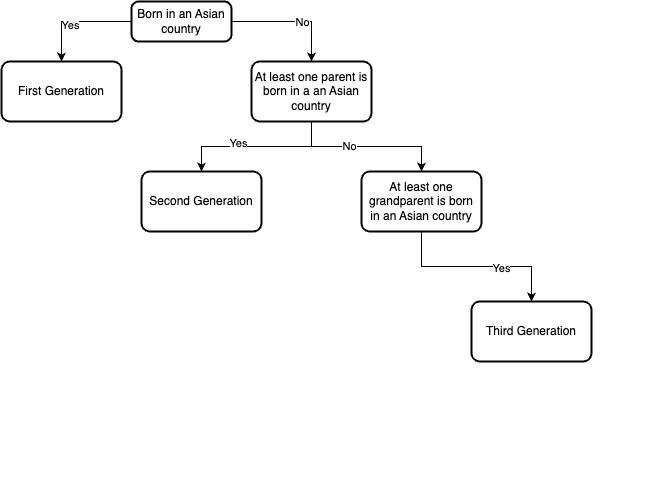
\includegraphics[width=\textwidth, height=9cm]{figure/diag.png} 
\label{fig:diag}
\end{figure}
\hfill%
\end{center}


My analysis depends on a sub sample of the US population, I show in table (\ref{tab:hispbygen}) that I have enough observations in each generation. Consistent with the literature on ethnic attrition among Hispanics, I find significant attrition among third-generation Hispanic immigrants.\footnote{In \citet{duncanIdentifyingLaterGenerationDescendants2018,duncanSocioeconomicIntegrationImmigrant2018, antmanEthnicAttritionObserved2016,antmanEthnicAttritionAssimilation2020}, the authors find substantial attrition among Hispanics.} These results are displayed in table (\ref{tab:hispbygen}): most first- and second-generation Hispanic immigrants self-reportedly identified as Hispanic. Of the first-generation Hispanic immigrants, 96\% self-reportedly identified as Hispanic. Similarly, 95\% of the second-generation Hispanic immigrants self-reportedly identified as Hispanic, and 85\% of third-generation Hispanic immigrants identifying as Hispanic. That is a more than threefold increase in attrition rates. Most of the attrition among third-generation Hispanics is driven by attrition among the children of inter-ethnic marriages.


\begin{table}[H]
\centering\centering
\caption{Asian Self-identification by Generation \label{tab:hispbygen}}
\centering
\begin{threeparttable}
\begin{tabular}[t]{>{}lcccc}
\toprule
  & \specialcell{Self-identify \\ as Asian} & \specialcell{Self-identify as \\ non-Asian} & \specialcell{\% Self-identify \\ as Asian} & \specialcell{\% Self-identify \\ as non-Asian}\\
\midrule
\textbf{1st Gen.} & 14,811 & 688 & 0.96 & 0.04\\
\textbf{2nd Gen.} & 58,756 & 21,381 & 0.73 & 0.27\\
\hspace{1em}\textbf{Asian on:} &  &  &  \vphantom{1} & \\
\hspace{1em}\hspace{1em}\textbf{Both Sides} & 49,118 & 1,717 & 0.97 & 0.03\\
\hspace{1em}\hspace{1em}\textbf{One Side} & 9,638 & 19,664 & 0.33 & 0.67\\
\addlinespace
\textbf{3rd Gen.} & 10,394 & 23,048 & 0.31 & 0.69\\
\hspace{1em}\textbf{Asian on:} &  &  &  & \\
\hspace{1em}\hspace{1em}\textbf{Both Sides} & 5,428 & 316 & 0.94 & 0.06\\
\hspace{1em}\hspace{1em}\textbf{One Side} & 3,030 & 9,213 & 0.25 & 0.75\\
\bottomrule
\end{tabular}
\begin{tablenotes}
\item[1] The samples include children ages 17 and below who live in intact families. First-generation Asian immigrant children that were born in a Asian country. Native-born second-generation Asian immigrant children with at least one parent born in a Asian country. Finally, native-born third-generation Asian immigrant children with native-born parents and at least one grandparent born in a Asian country.
\item[2] Data source is the 2004-2021 Current Population Survey.
\end{tablenotes}
\end{threeparttable}
\end{table}


\begin{center}
\begin{figure}[H]
\caption{Bias and Self-reported Hispanic Identity in the Least and Most Biased Places}

% first
\begin{subfigure}{.9\textwidth}
\caption{Skin Tone Implicit Association Bias Over Time}
\centering
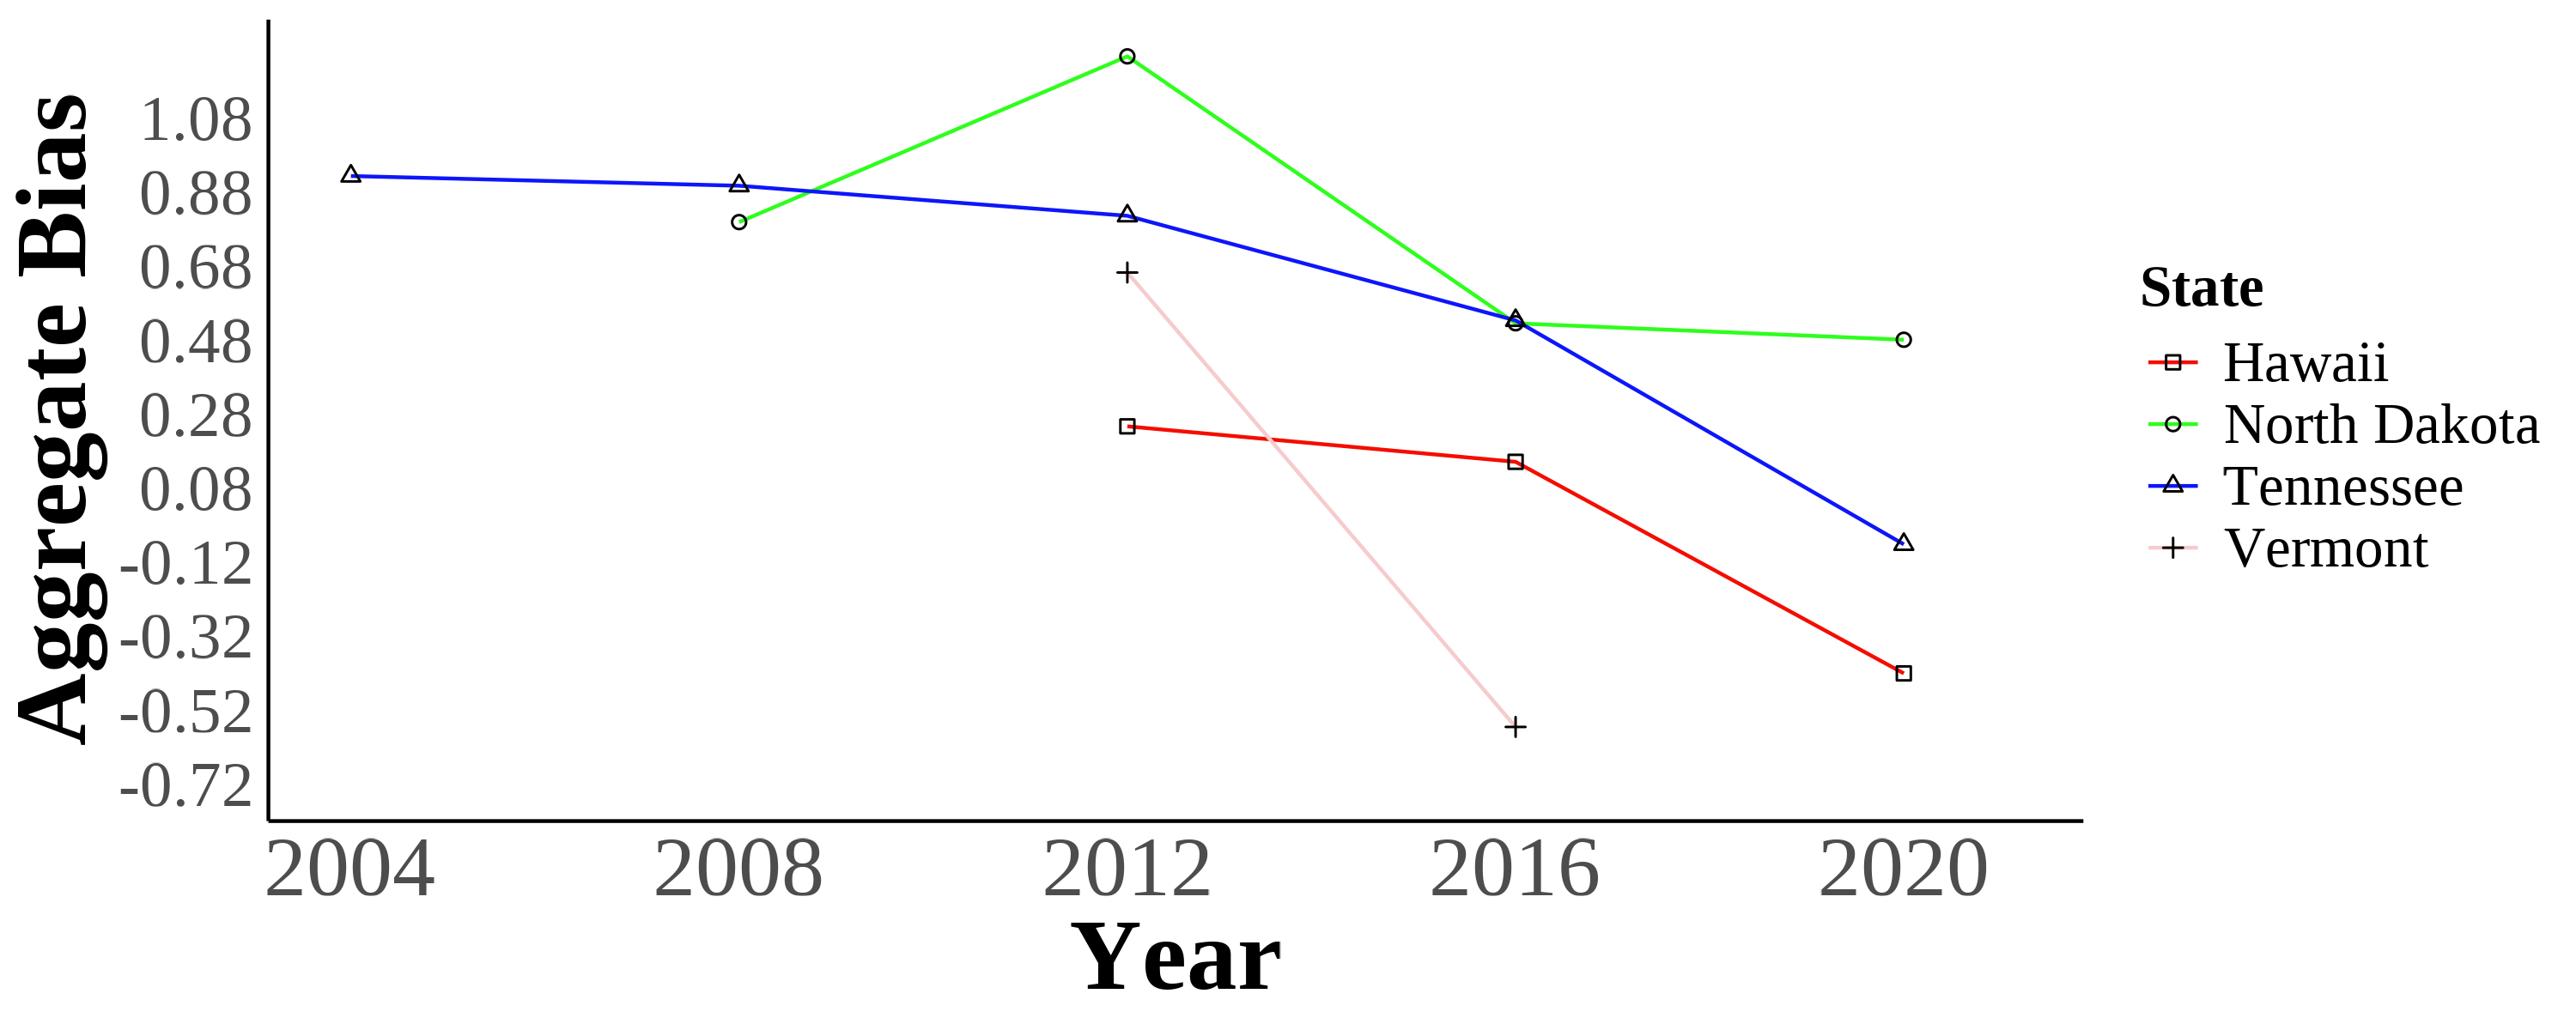
\includegraphics[width=.9\linewidth]{figure/Bias_twostates.png} 
\label{fig:skiniat}
\end{subfigure}
% Second
\begin{subfigure}{.9\textwidth}
\caption{Self-reported Hispanic Identity Over Time}
\centering
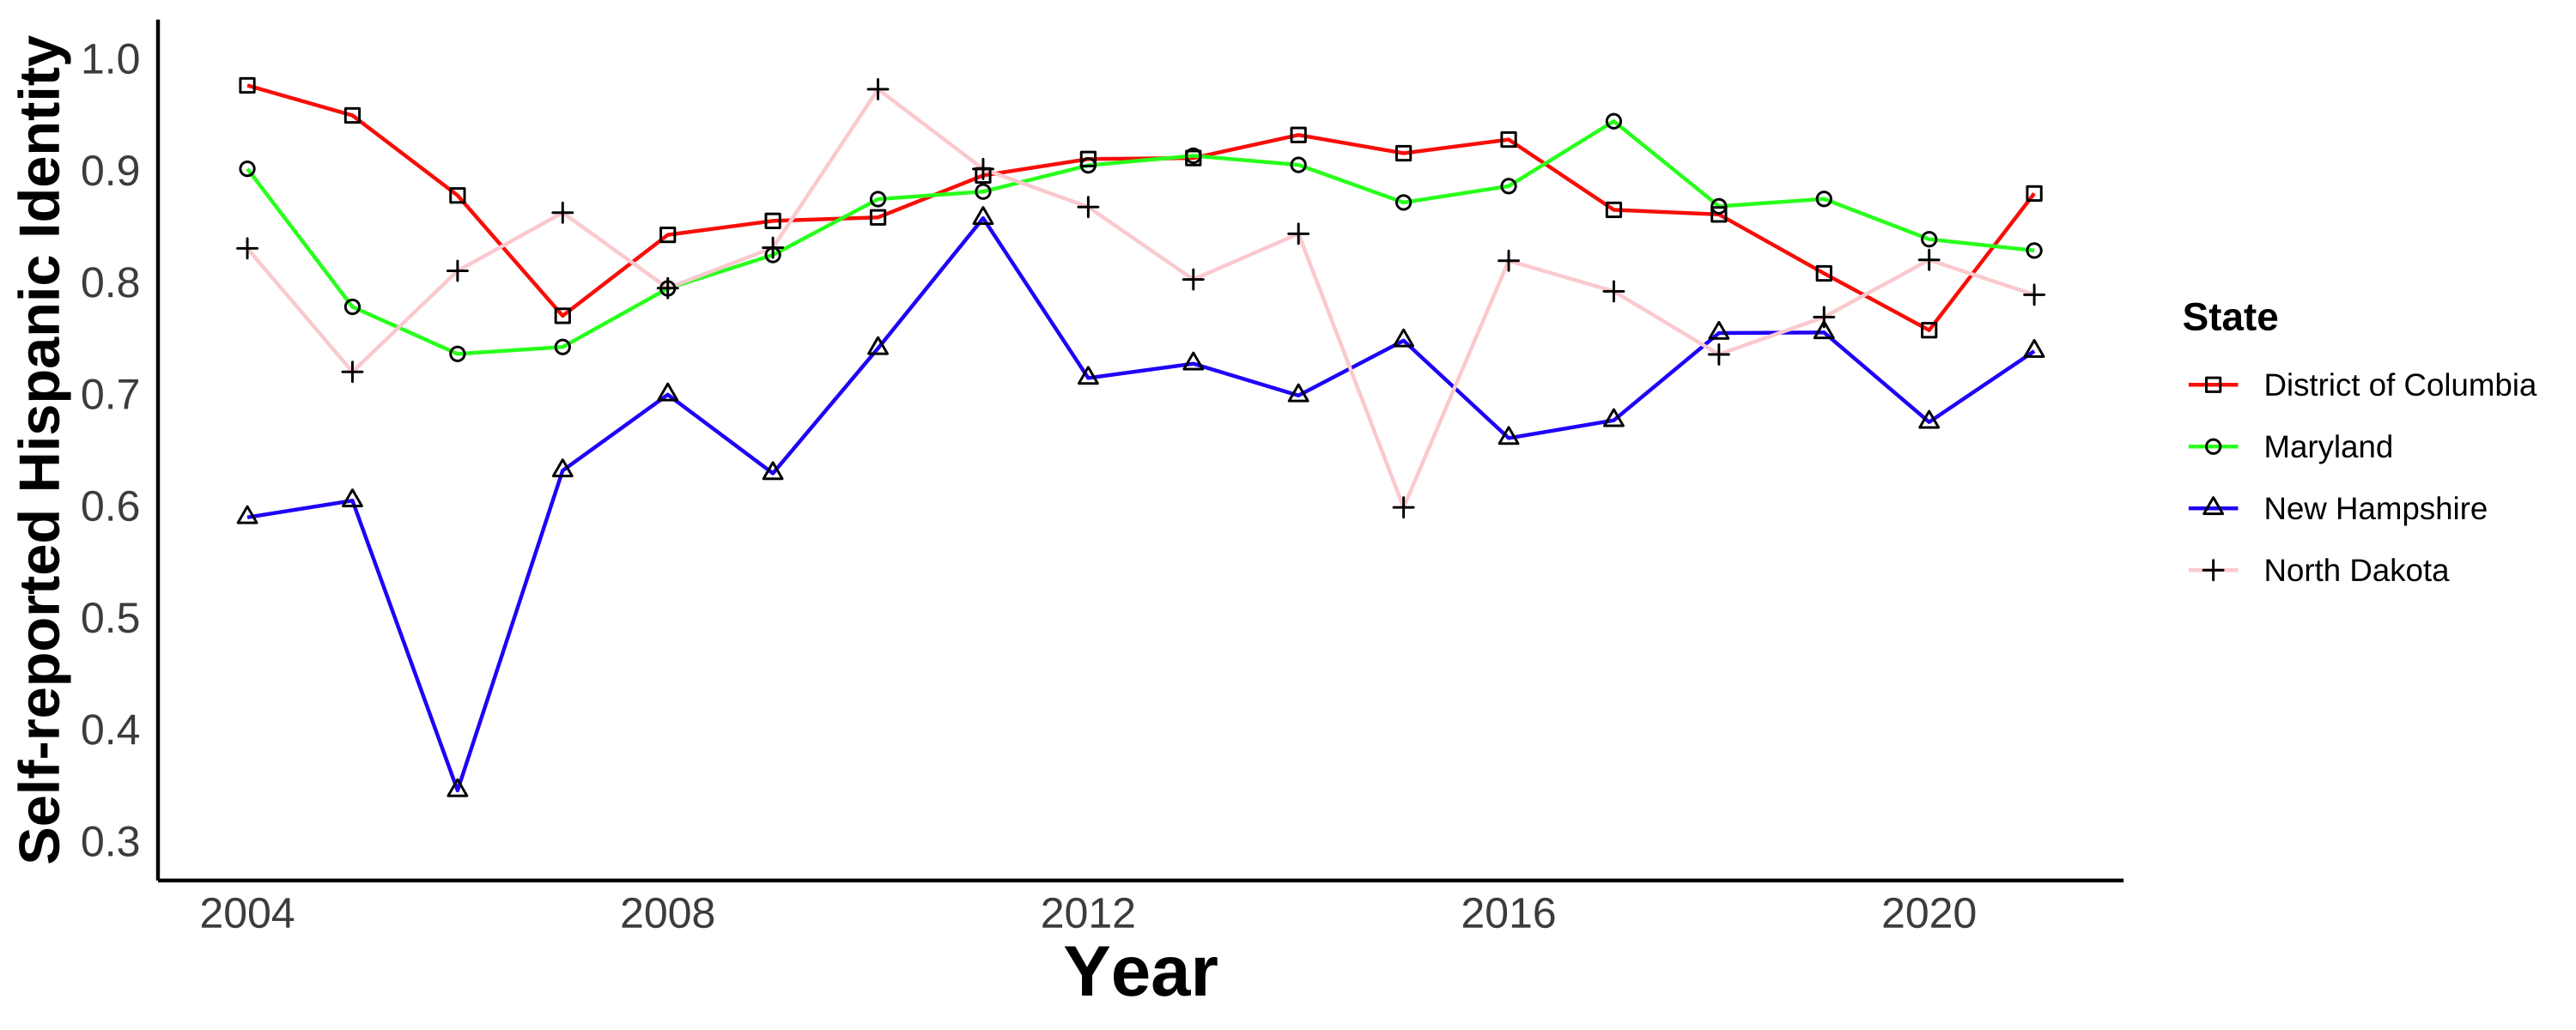
\includegraphics[width=.9\linewidth]{figure/Bias_twostates-hisp.png} 
\label{fig:hispanic-twostates}
\end{subfigure}
\flushleft\footnotesize{\note{These two panels show the trends in implicit bias (panel a) and self-reported Hispanic identity among Hispanic immigrants (panel b) of the least and most biased places in the data. The District of Colombia is the least biased geographical area, and North Dakota is the most biased. The bias units are in standard deviations. Self-reported Hispanic identity is among first, second, and third-generation Hispanic immigrants aged 17 and younger still living in intact families.}\\
\note{Bias data is from the 2004-2021 Harvard's Project Implicit Association Test scores. Identity data is from the 2004-2021 Current Population Survey (CPS).}}
\end{figure}
\end{center}


\newpage
\pagebreak

\begin{center}
\begin{figure}[H]
\caption{Maps of State-level Implicit Association Test Bias Over Time Measure with Census Division Regional Boundaries}
\label{fig:skiniat-maps}
% first
\begin{subfigure}{.45\textwidth}
\caption{State-level Bias in 2004}
\centering
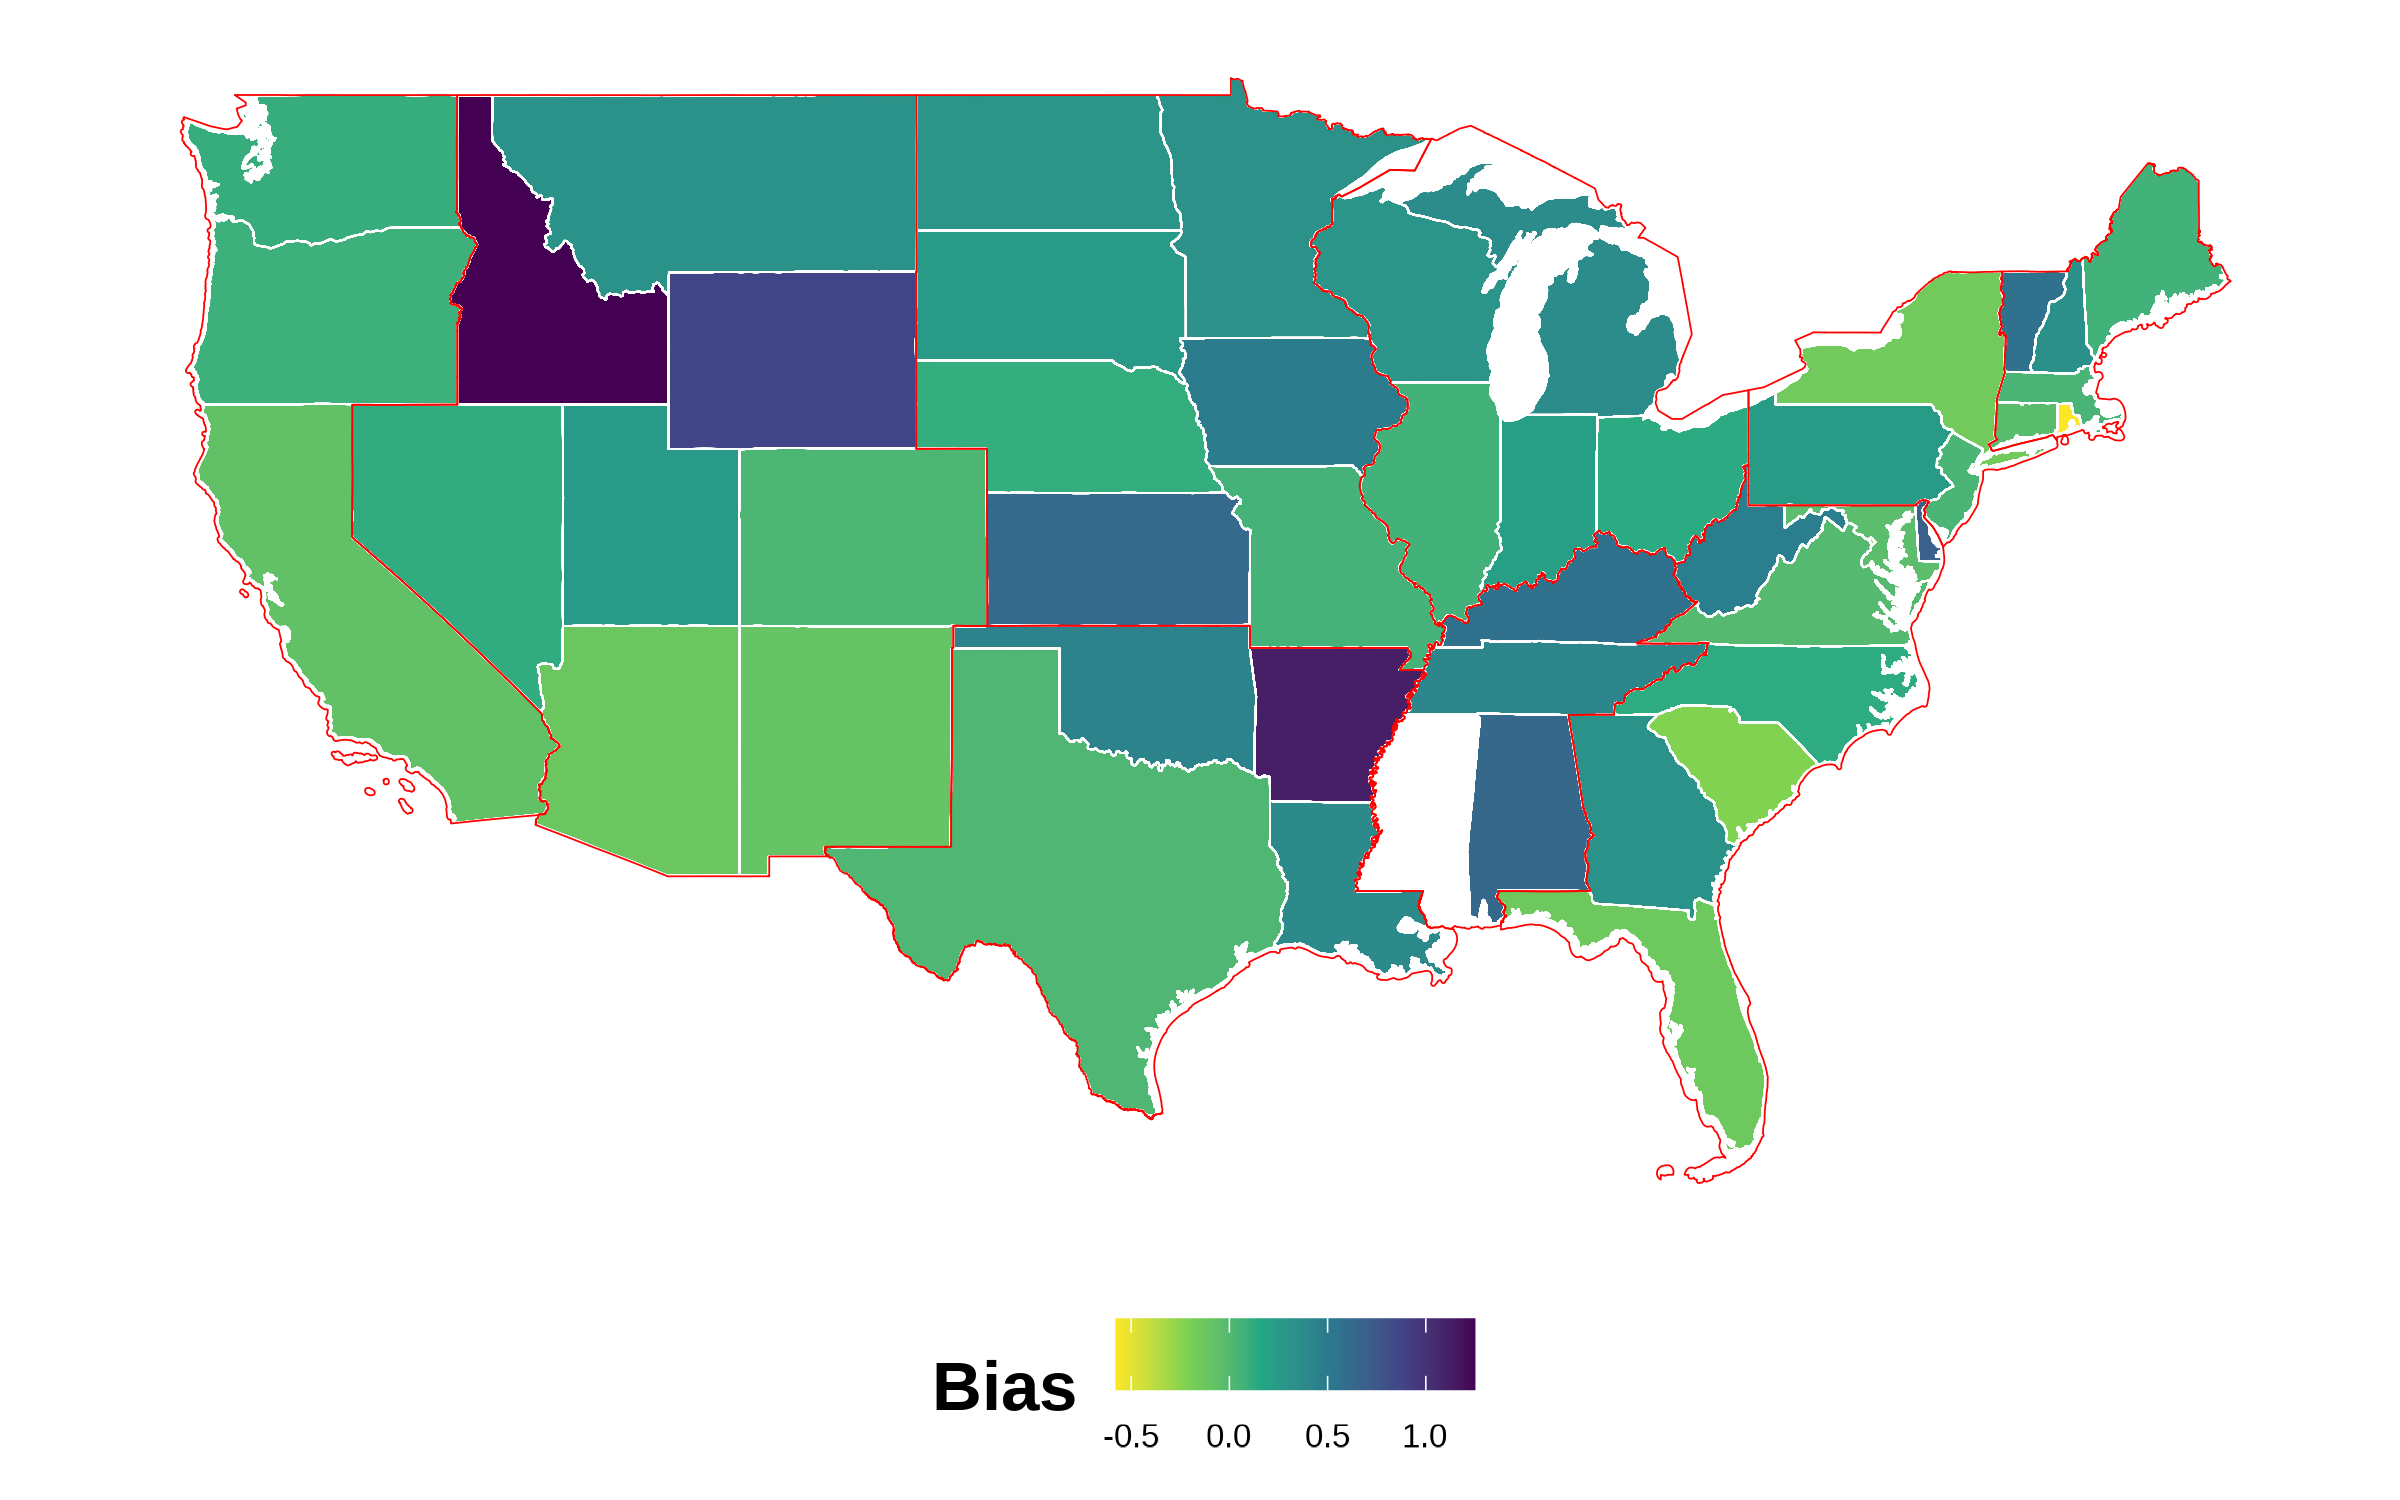
\includegraphics[width=0.9\linewidth]{figure/2004skinmap.png} 
\label{fig:skiniat-map-2004}
\end{subfigure}
\hfill%
% Second
\begin{subfigure}{.45\textwidth}
\caption{State-level Bias in 2006}
\centering
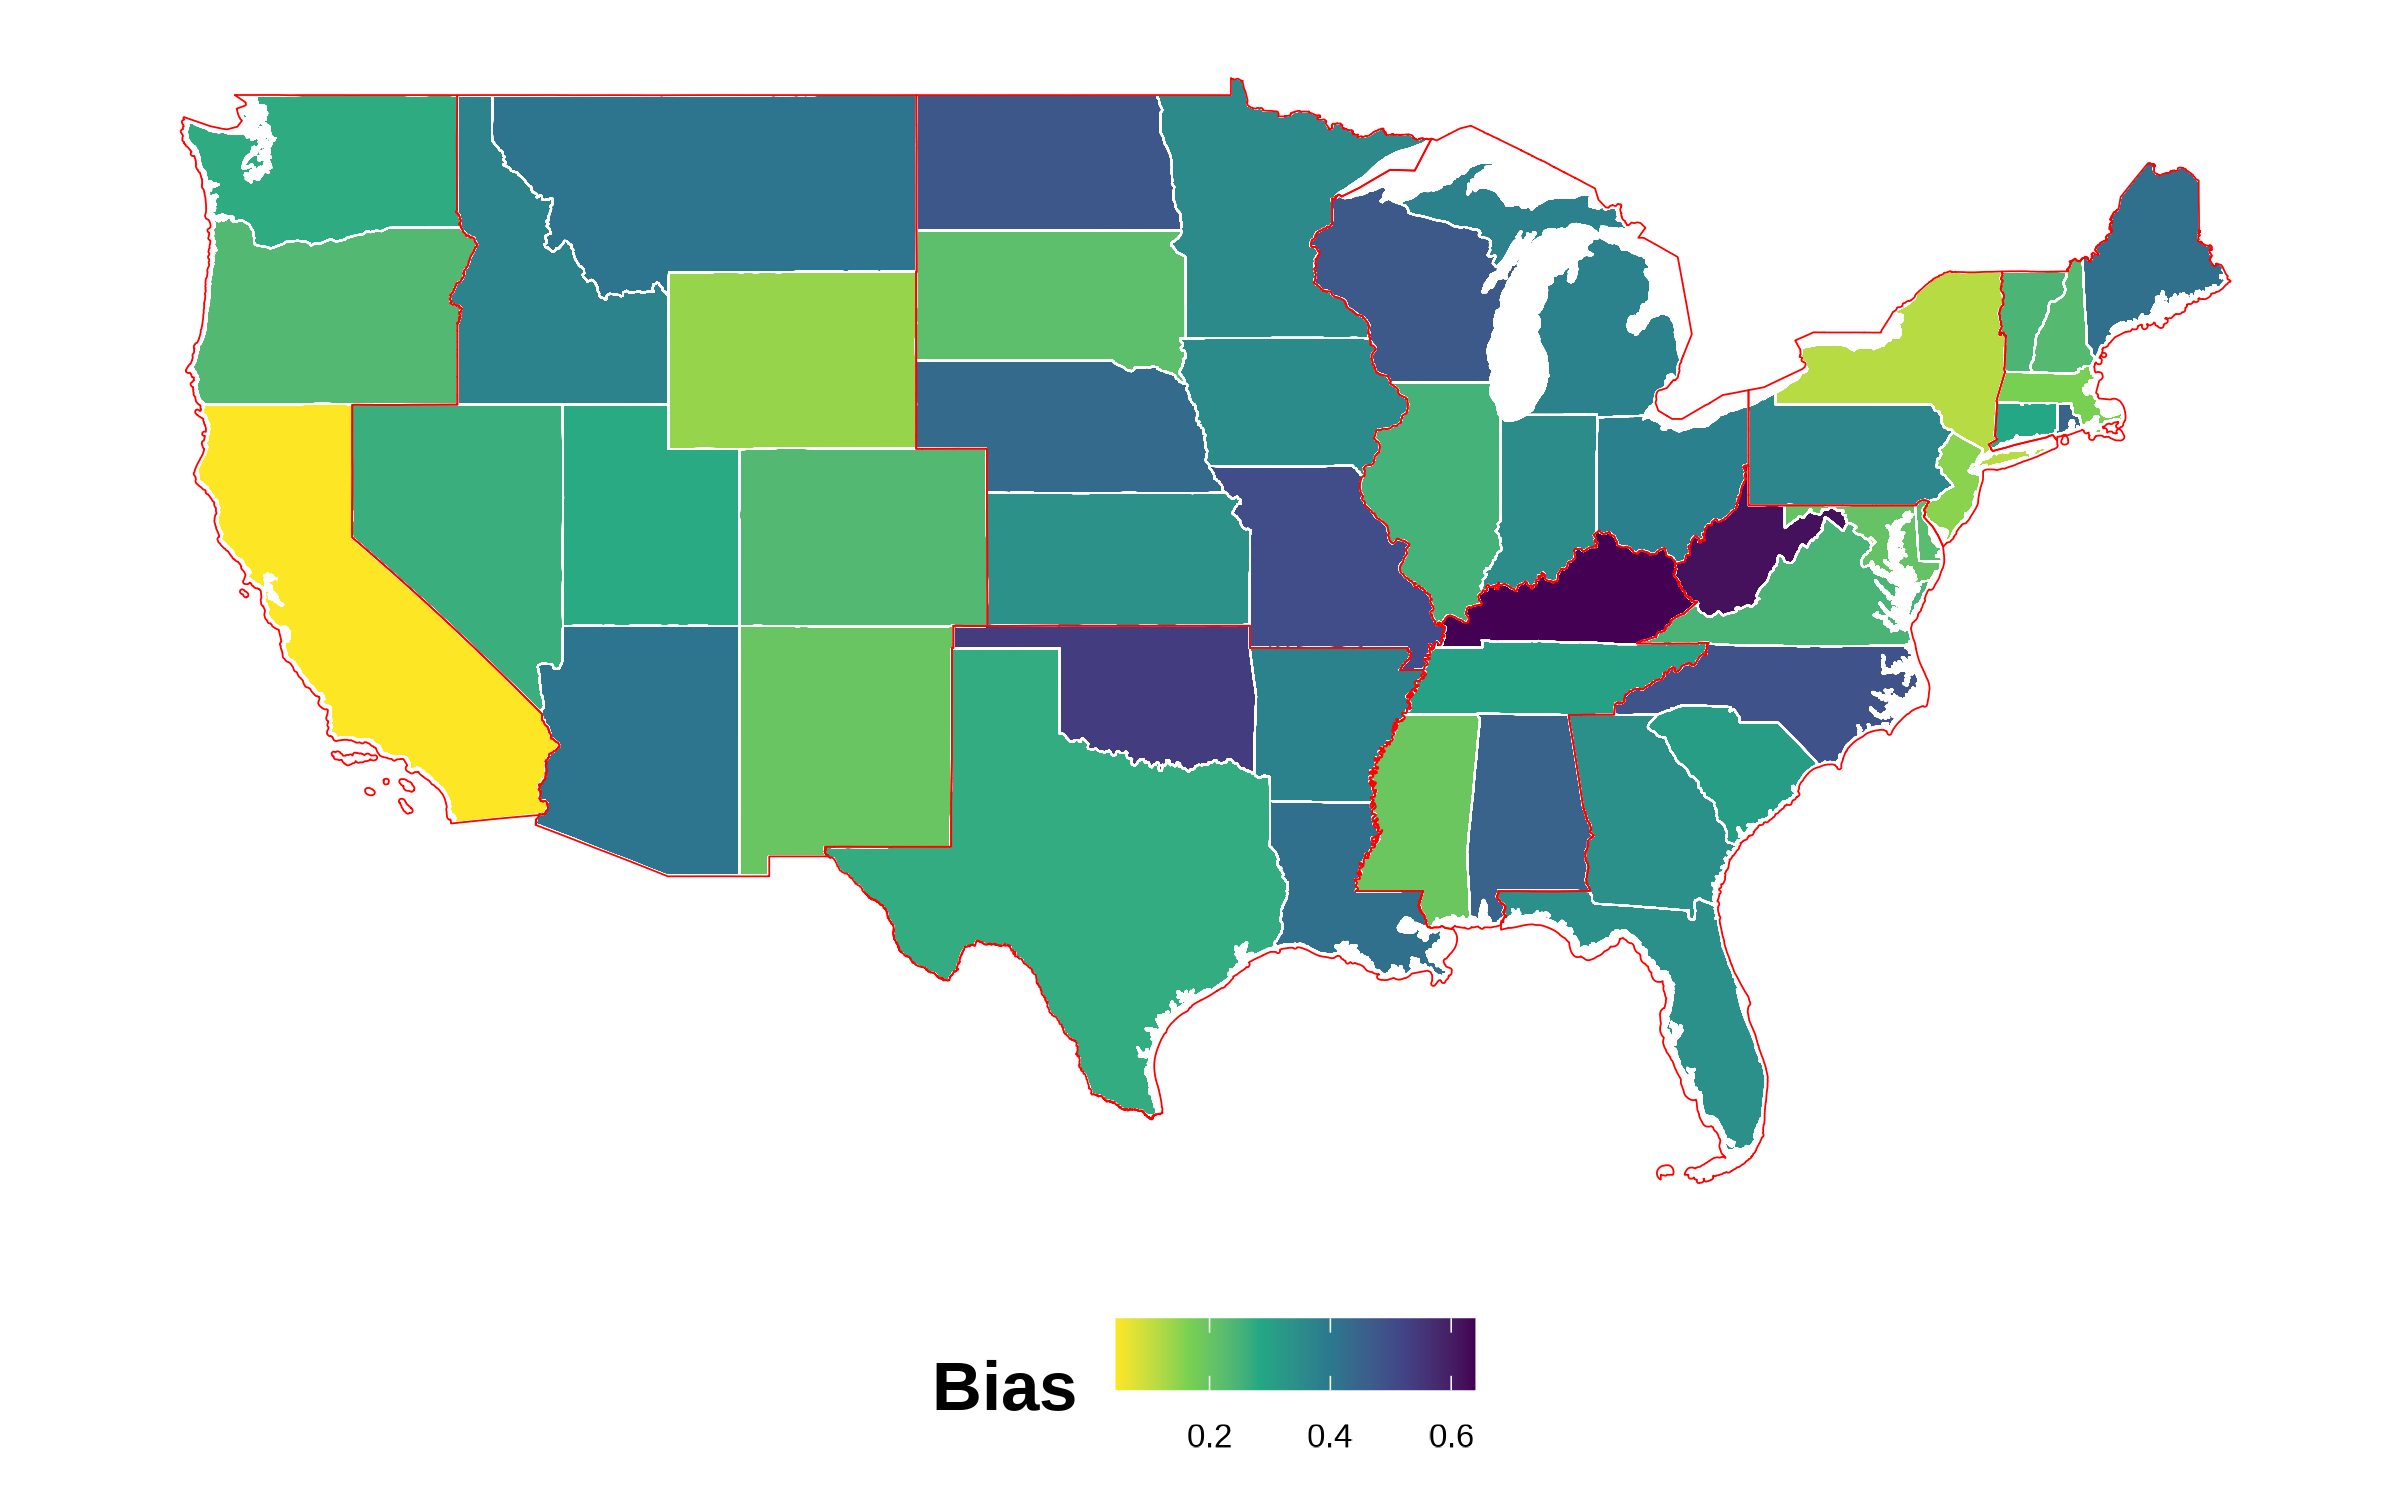
\includegraphics[width=0.9\linewidth]{figure/2006skinmap.png} 
\label{fig:skiniat-map-2006}
\end{subfigure}
\hfill%
% third
\begin{subfigure}{.45\textwidth}
\caption{State-level Bias in 2008}
\centering
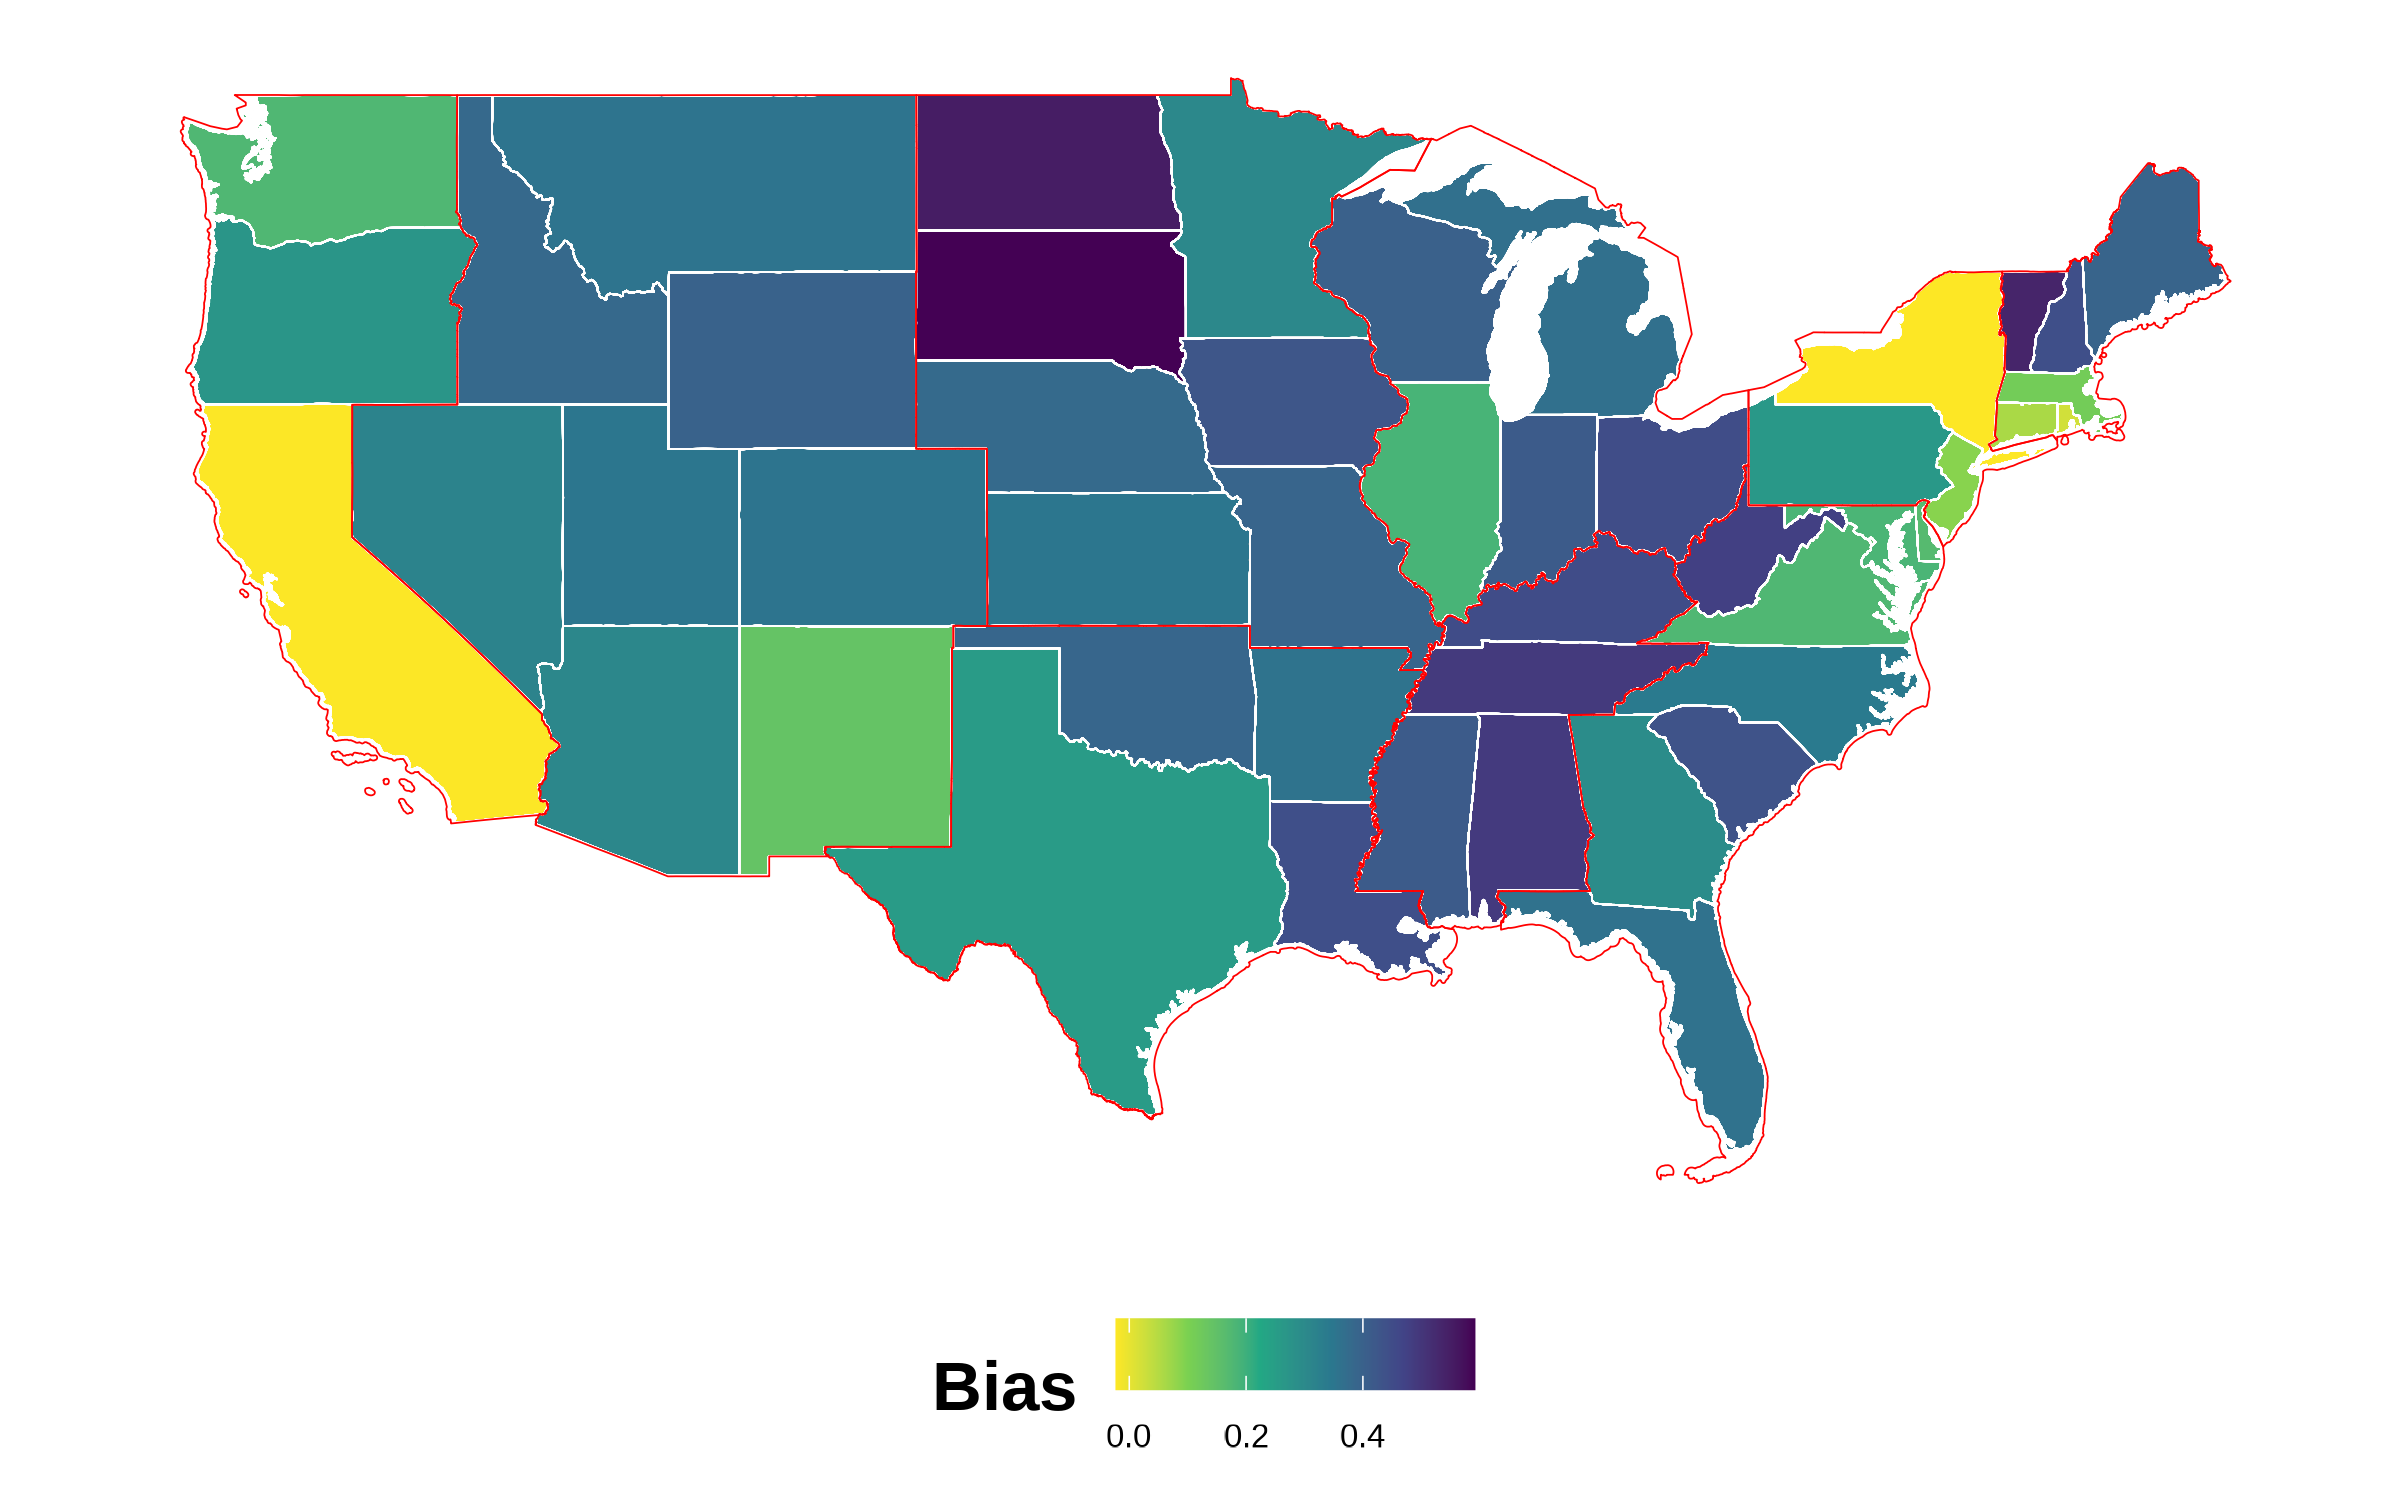
\includegraphics[width=0.9\linewidth]{figure/2008skinmap.png} 
\label{fig:skiniat-map-2008}
\end{subfigure}
\hfill%
% fourth
\begin{subfigure}{.45\textwidth}
\caption{State-level Bias in 2010}
\centering
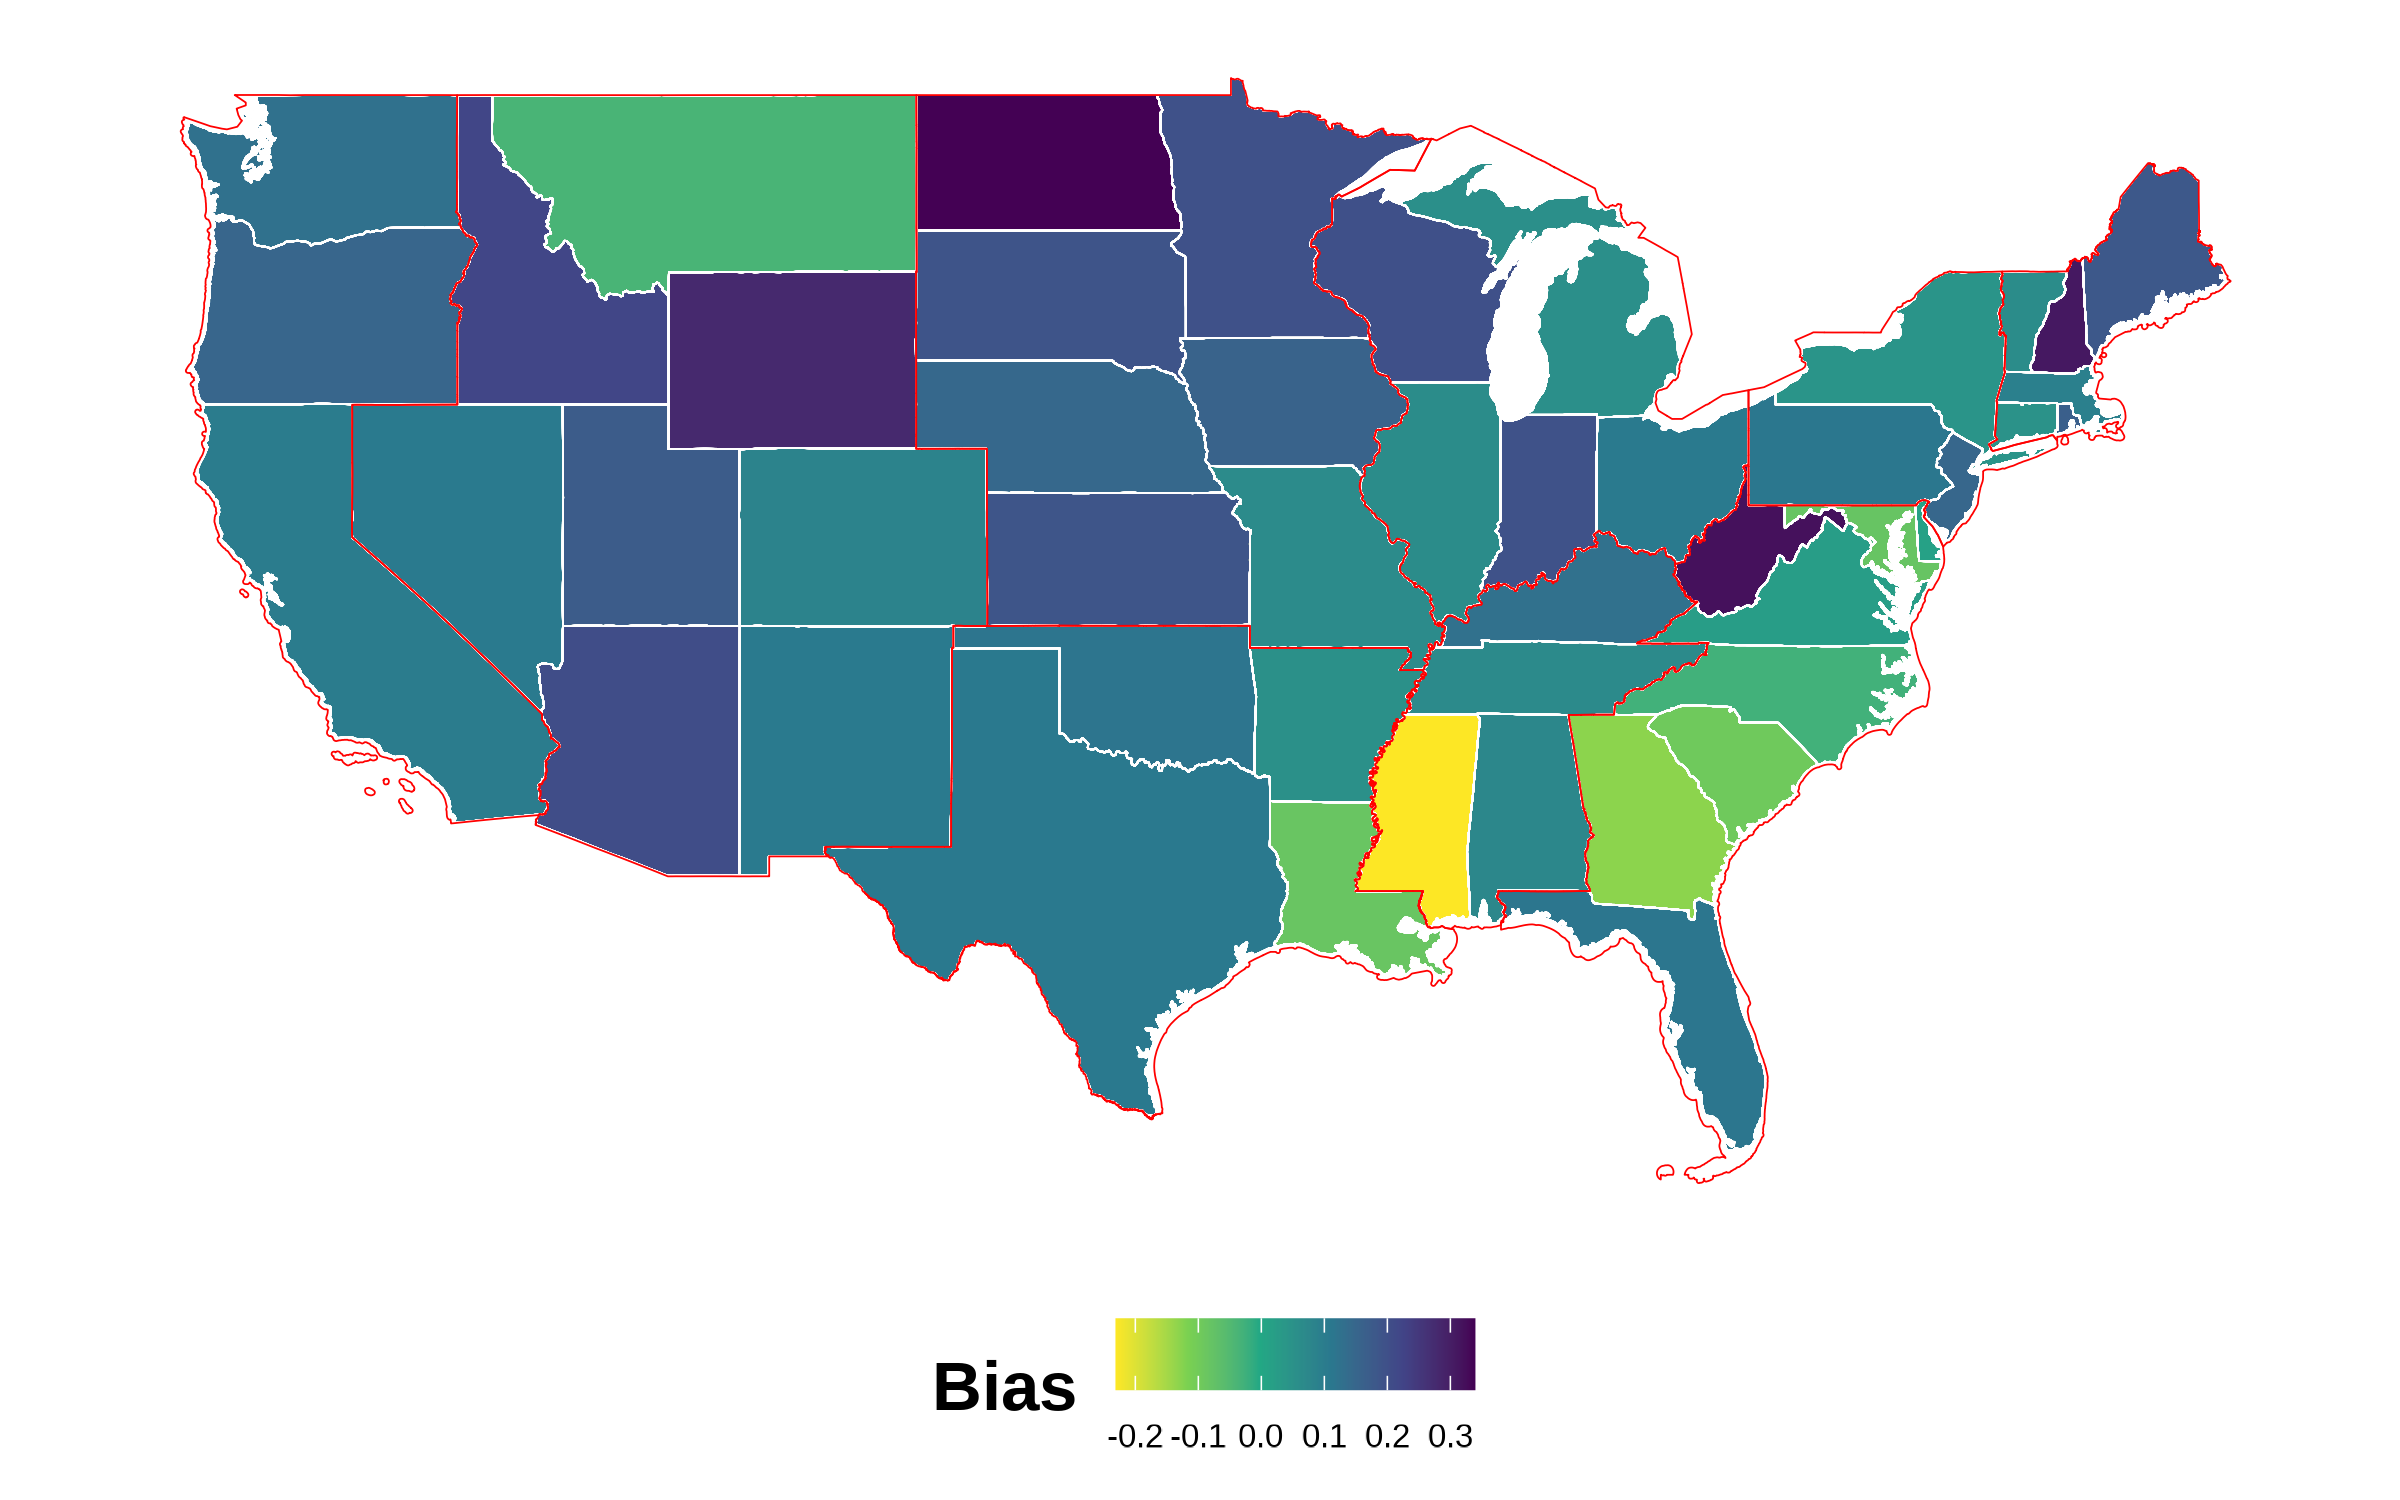
\includegraphics[width=0.9\linewidth]{figure/2010skinmap.png} 
\label{fig:skiniat-map-2010}
\end{subfigure}
\hfill%
% fifth
\begin{subfigure}{.45\textwidth}
\caption{State-level Bias in 2012}
\centering
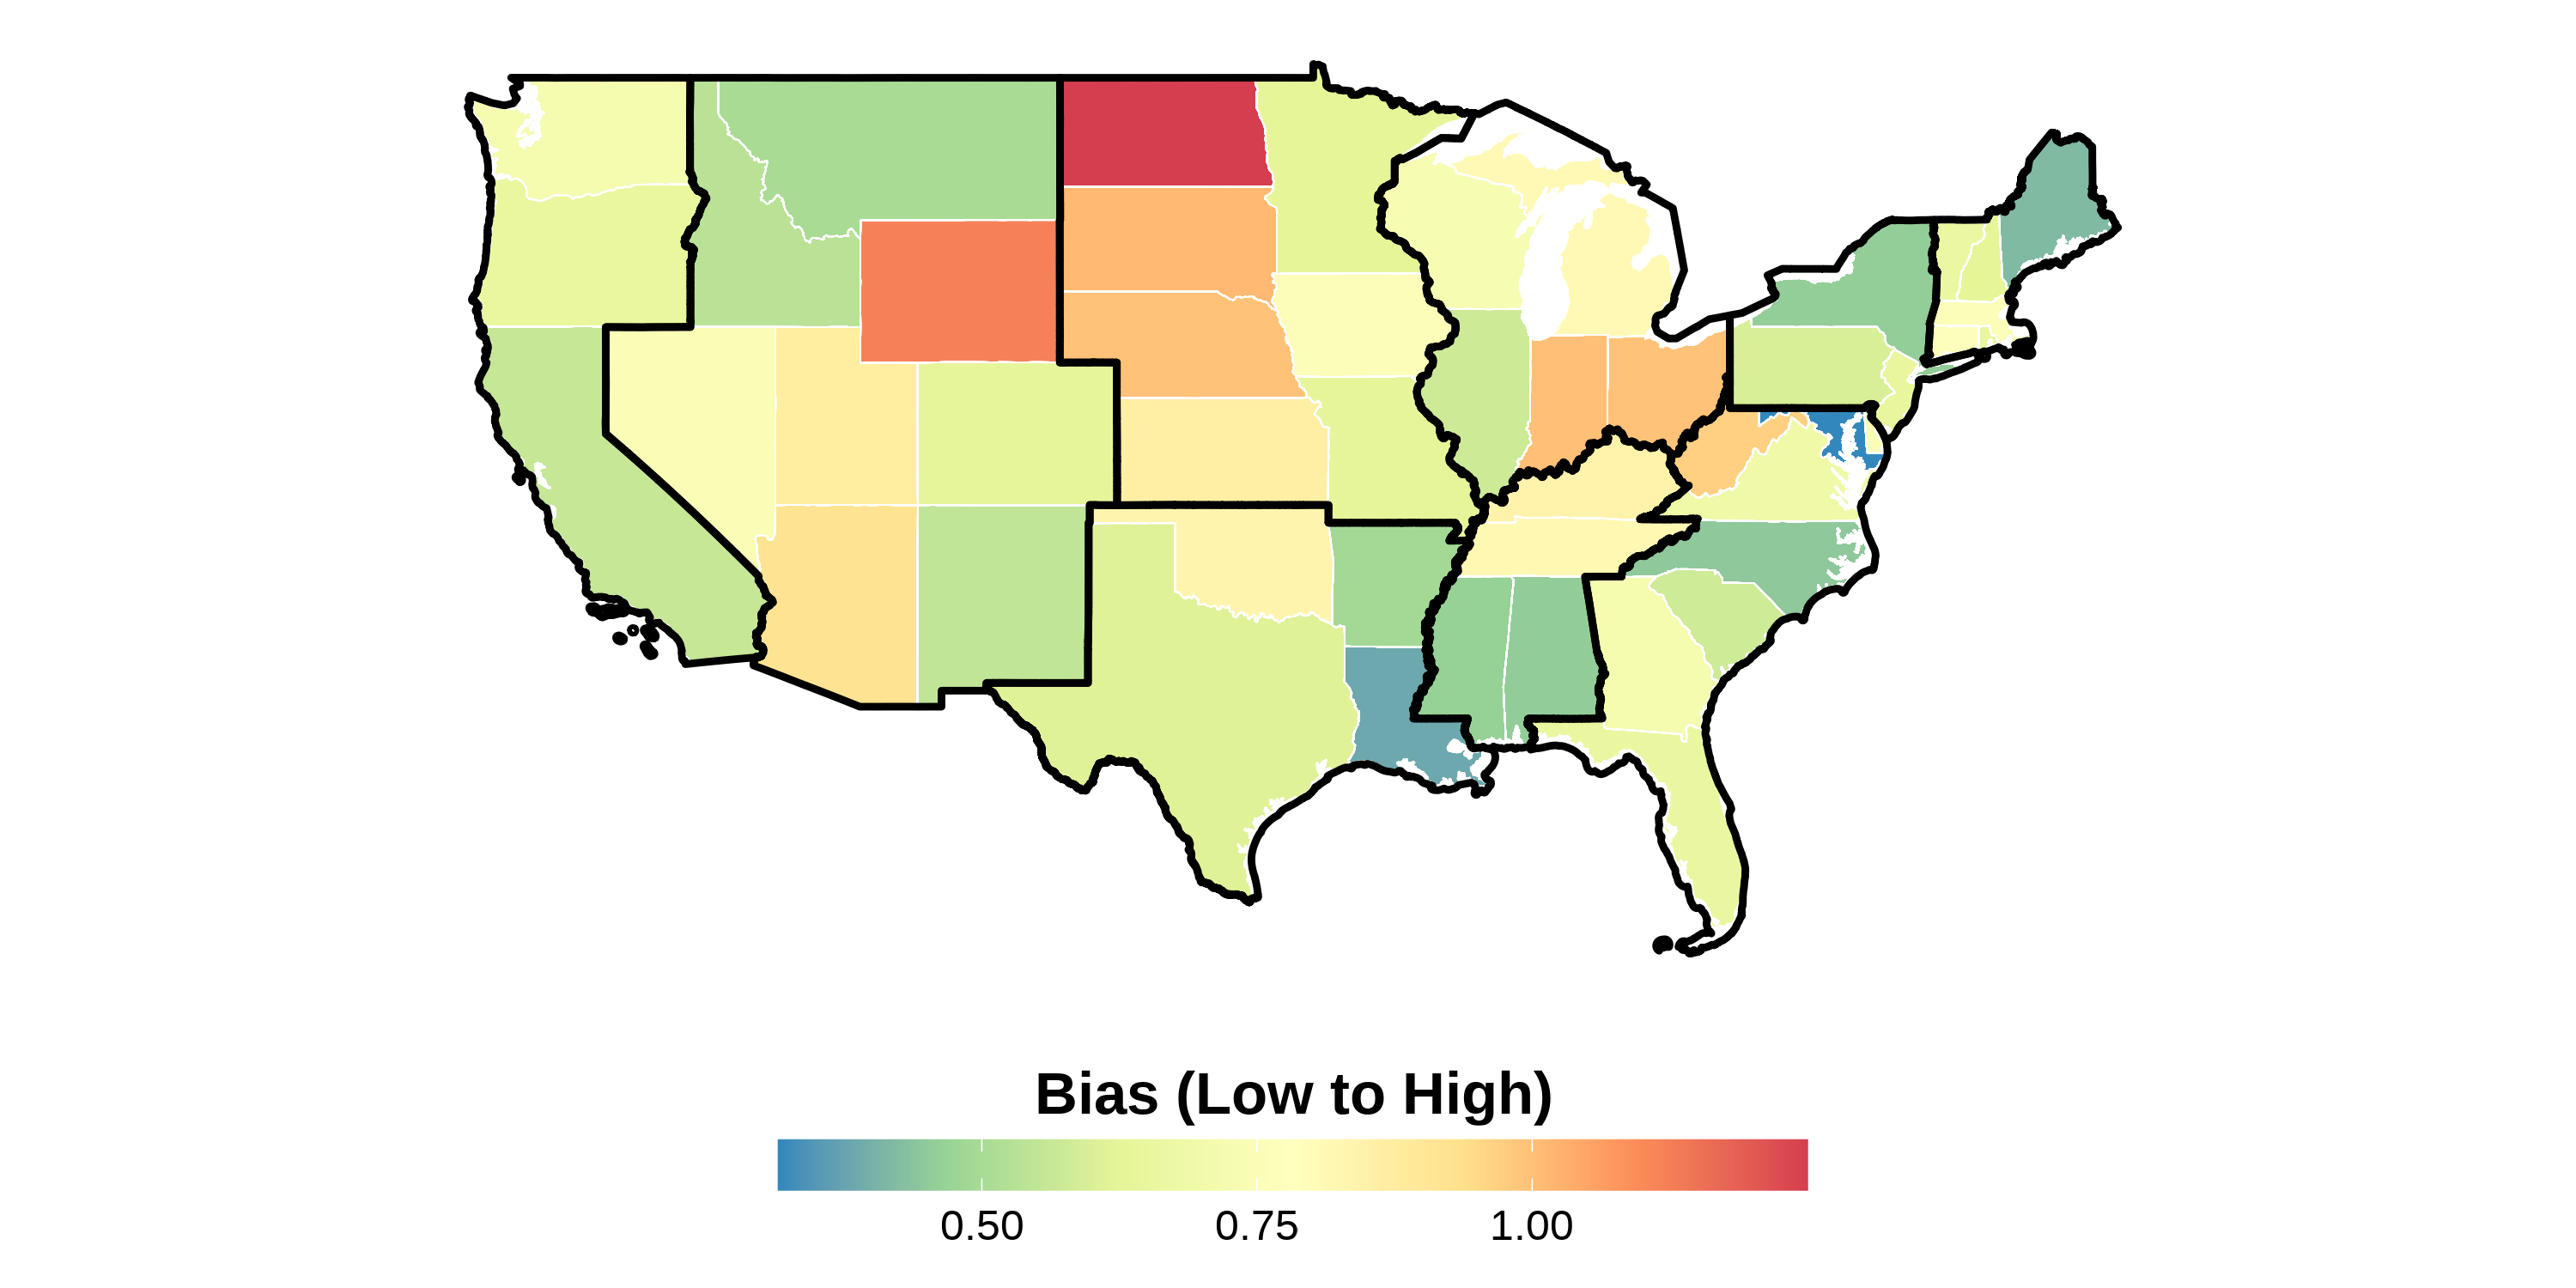
\includegraphics[width=0.9\linewidth]{figure/2012skinmap.png} 
\label{fig:skiniat-map-2012}
\end{subfigure}
\hfill%
% sixth
\begin{subfigure}{.45\textwidth}
\caption{State-level Bias in 2014}
\centering
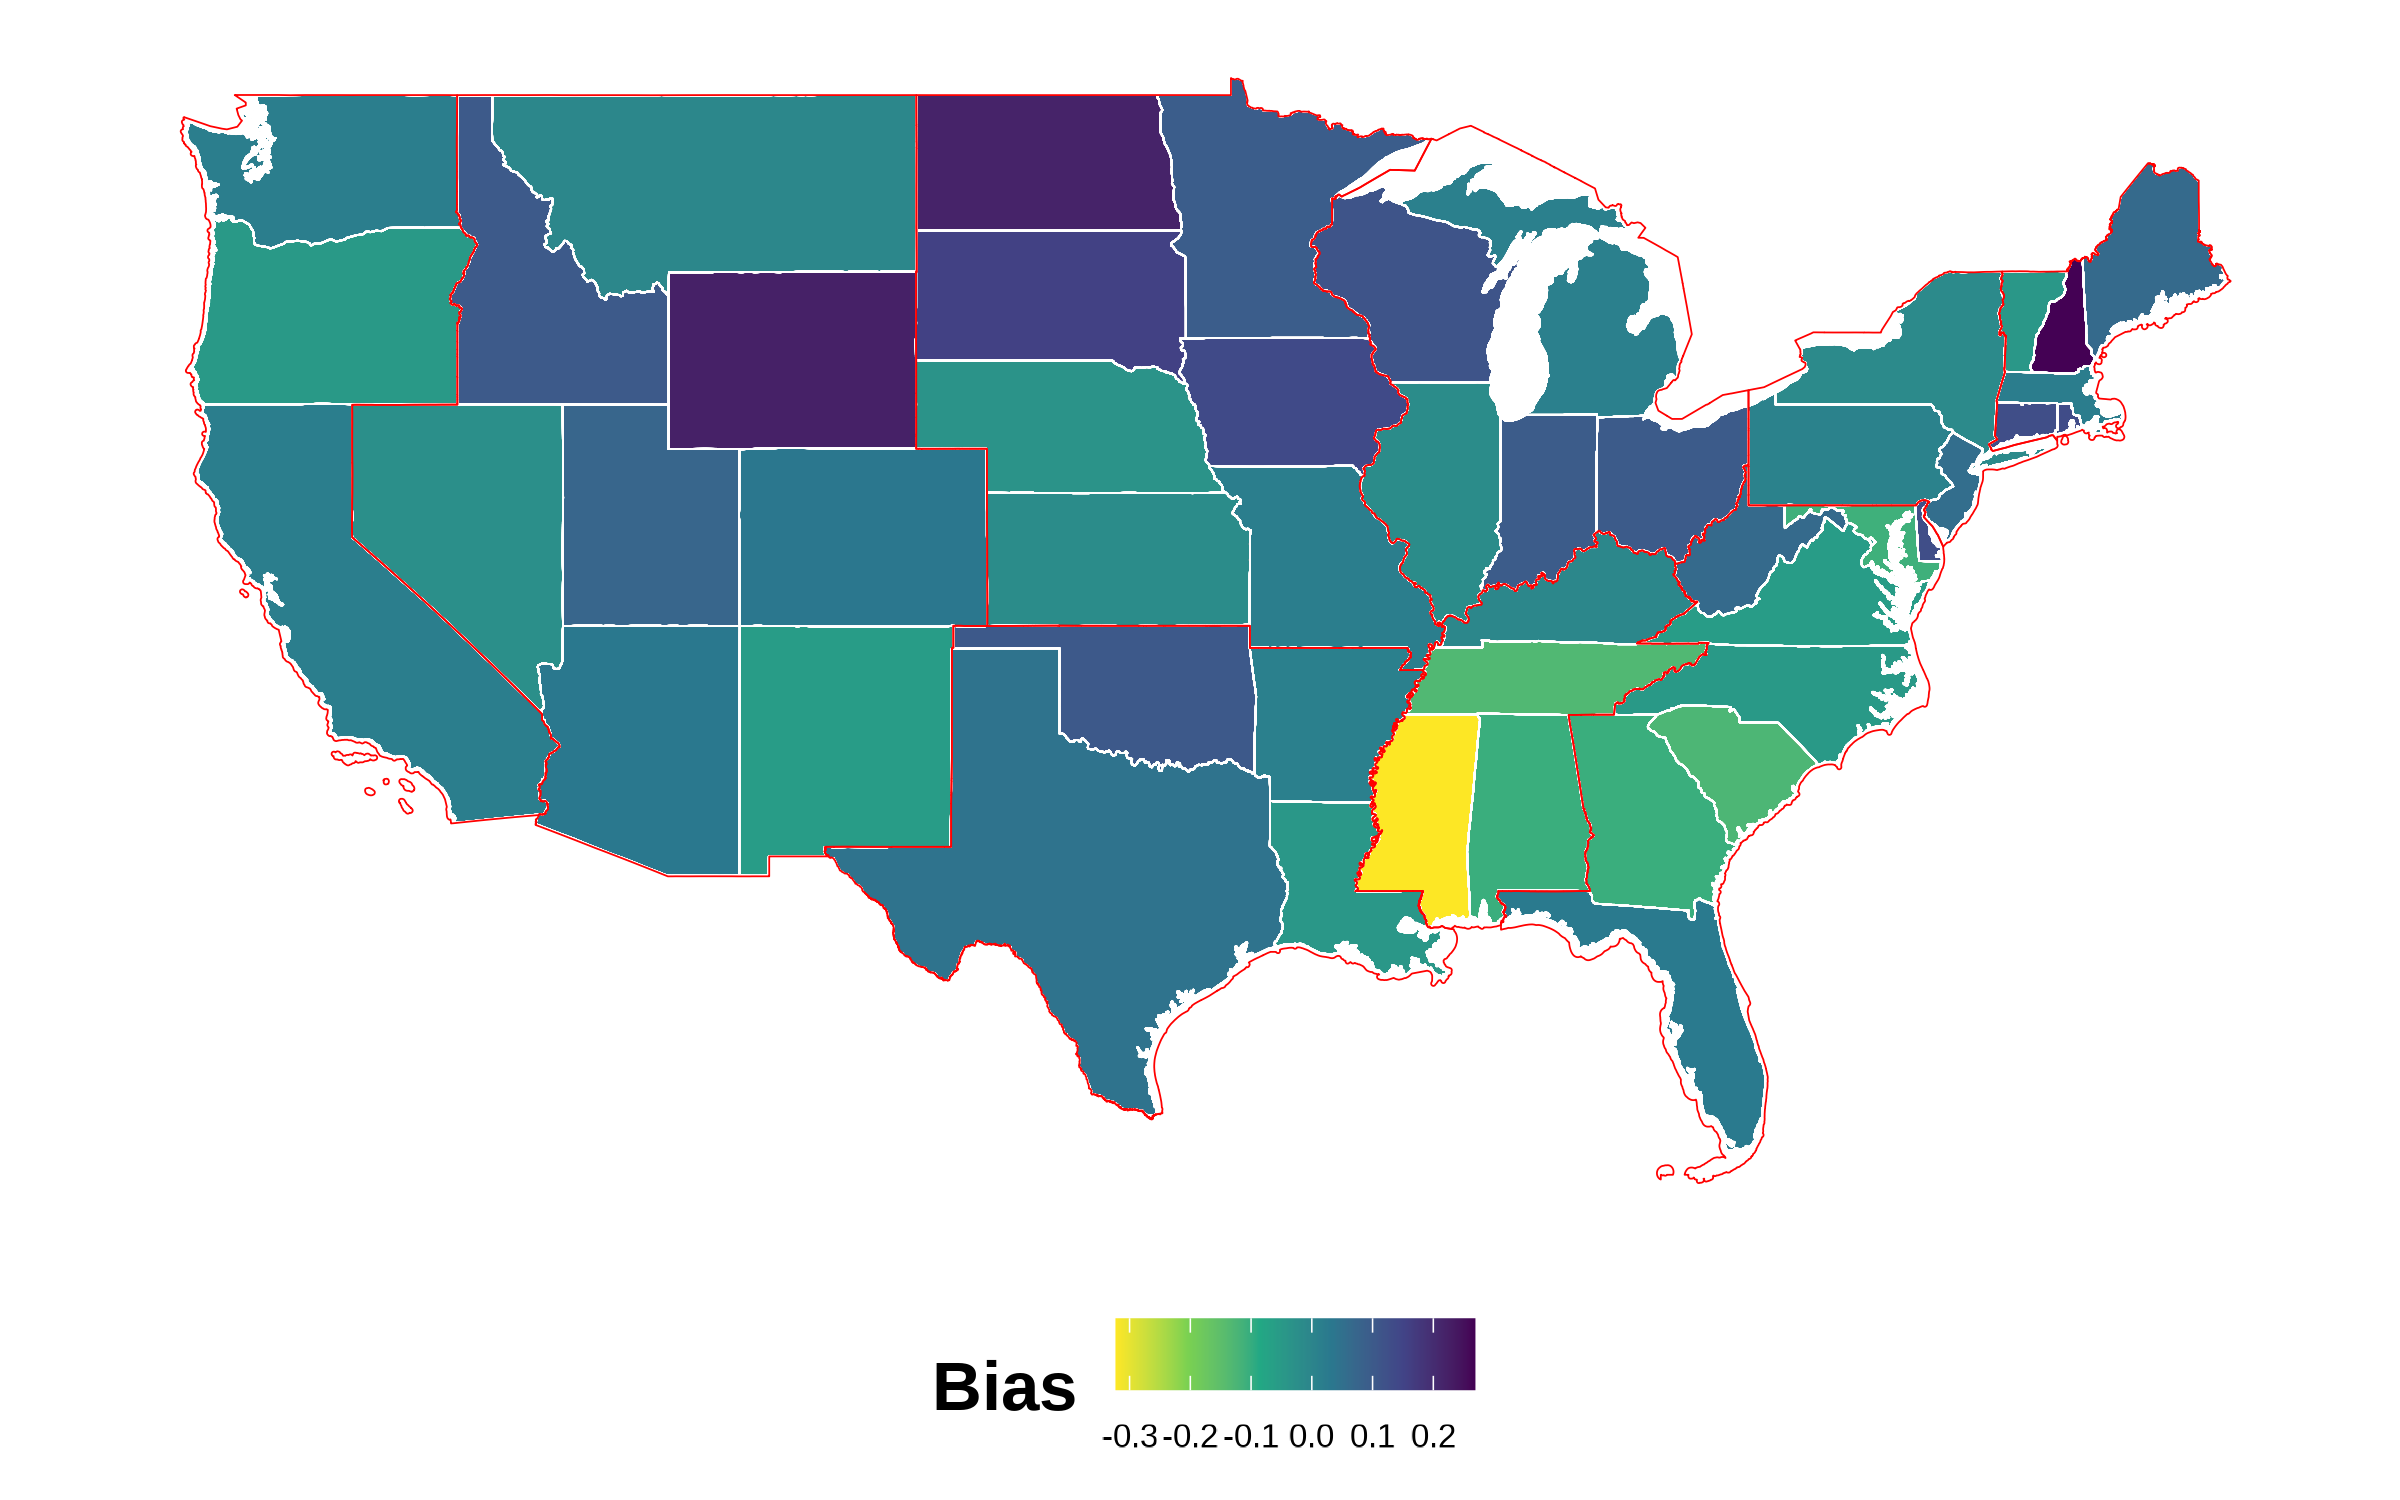
\includegraphics[width=0.9\linewidth]{figure/2014skinmap.png} 
\label{fig:skiniat-map-2014}
\end{subfigure}
\hfill%
% seventh
\begin{subfigure}{.45\textwidth}
\caption{State-level Bias in 2016}
\centering
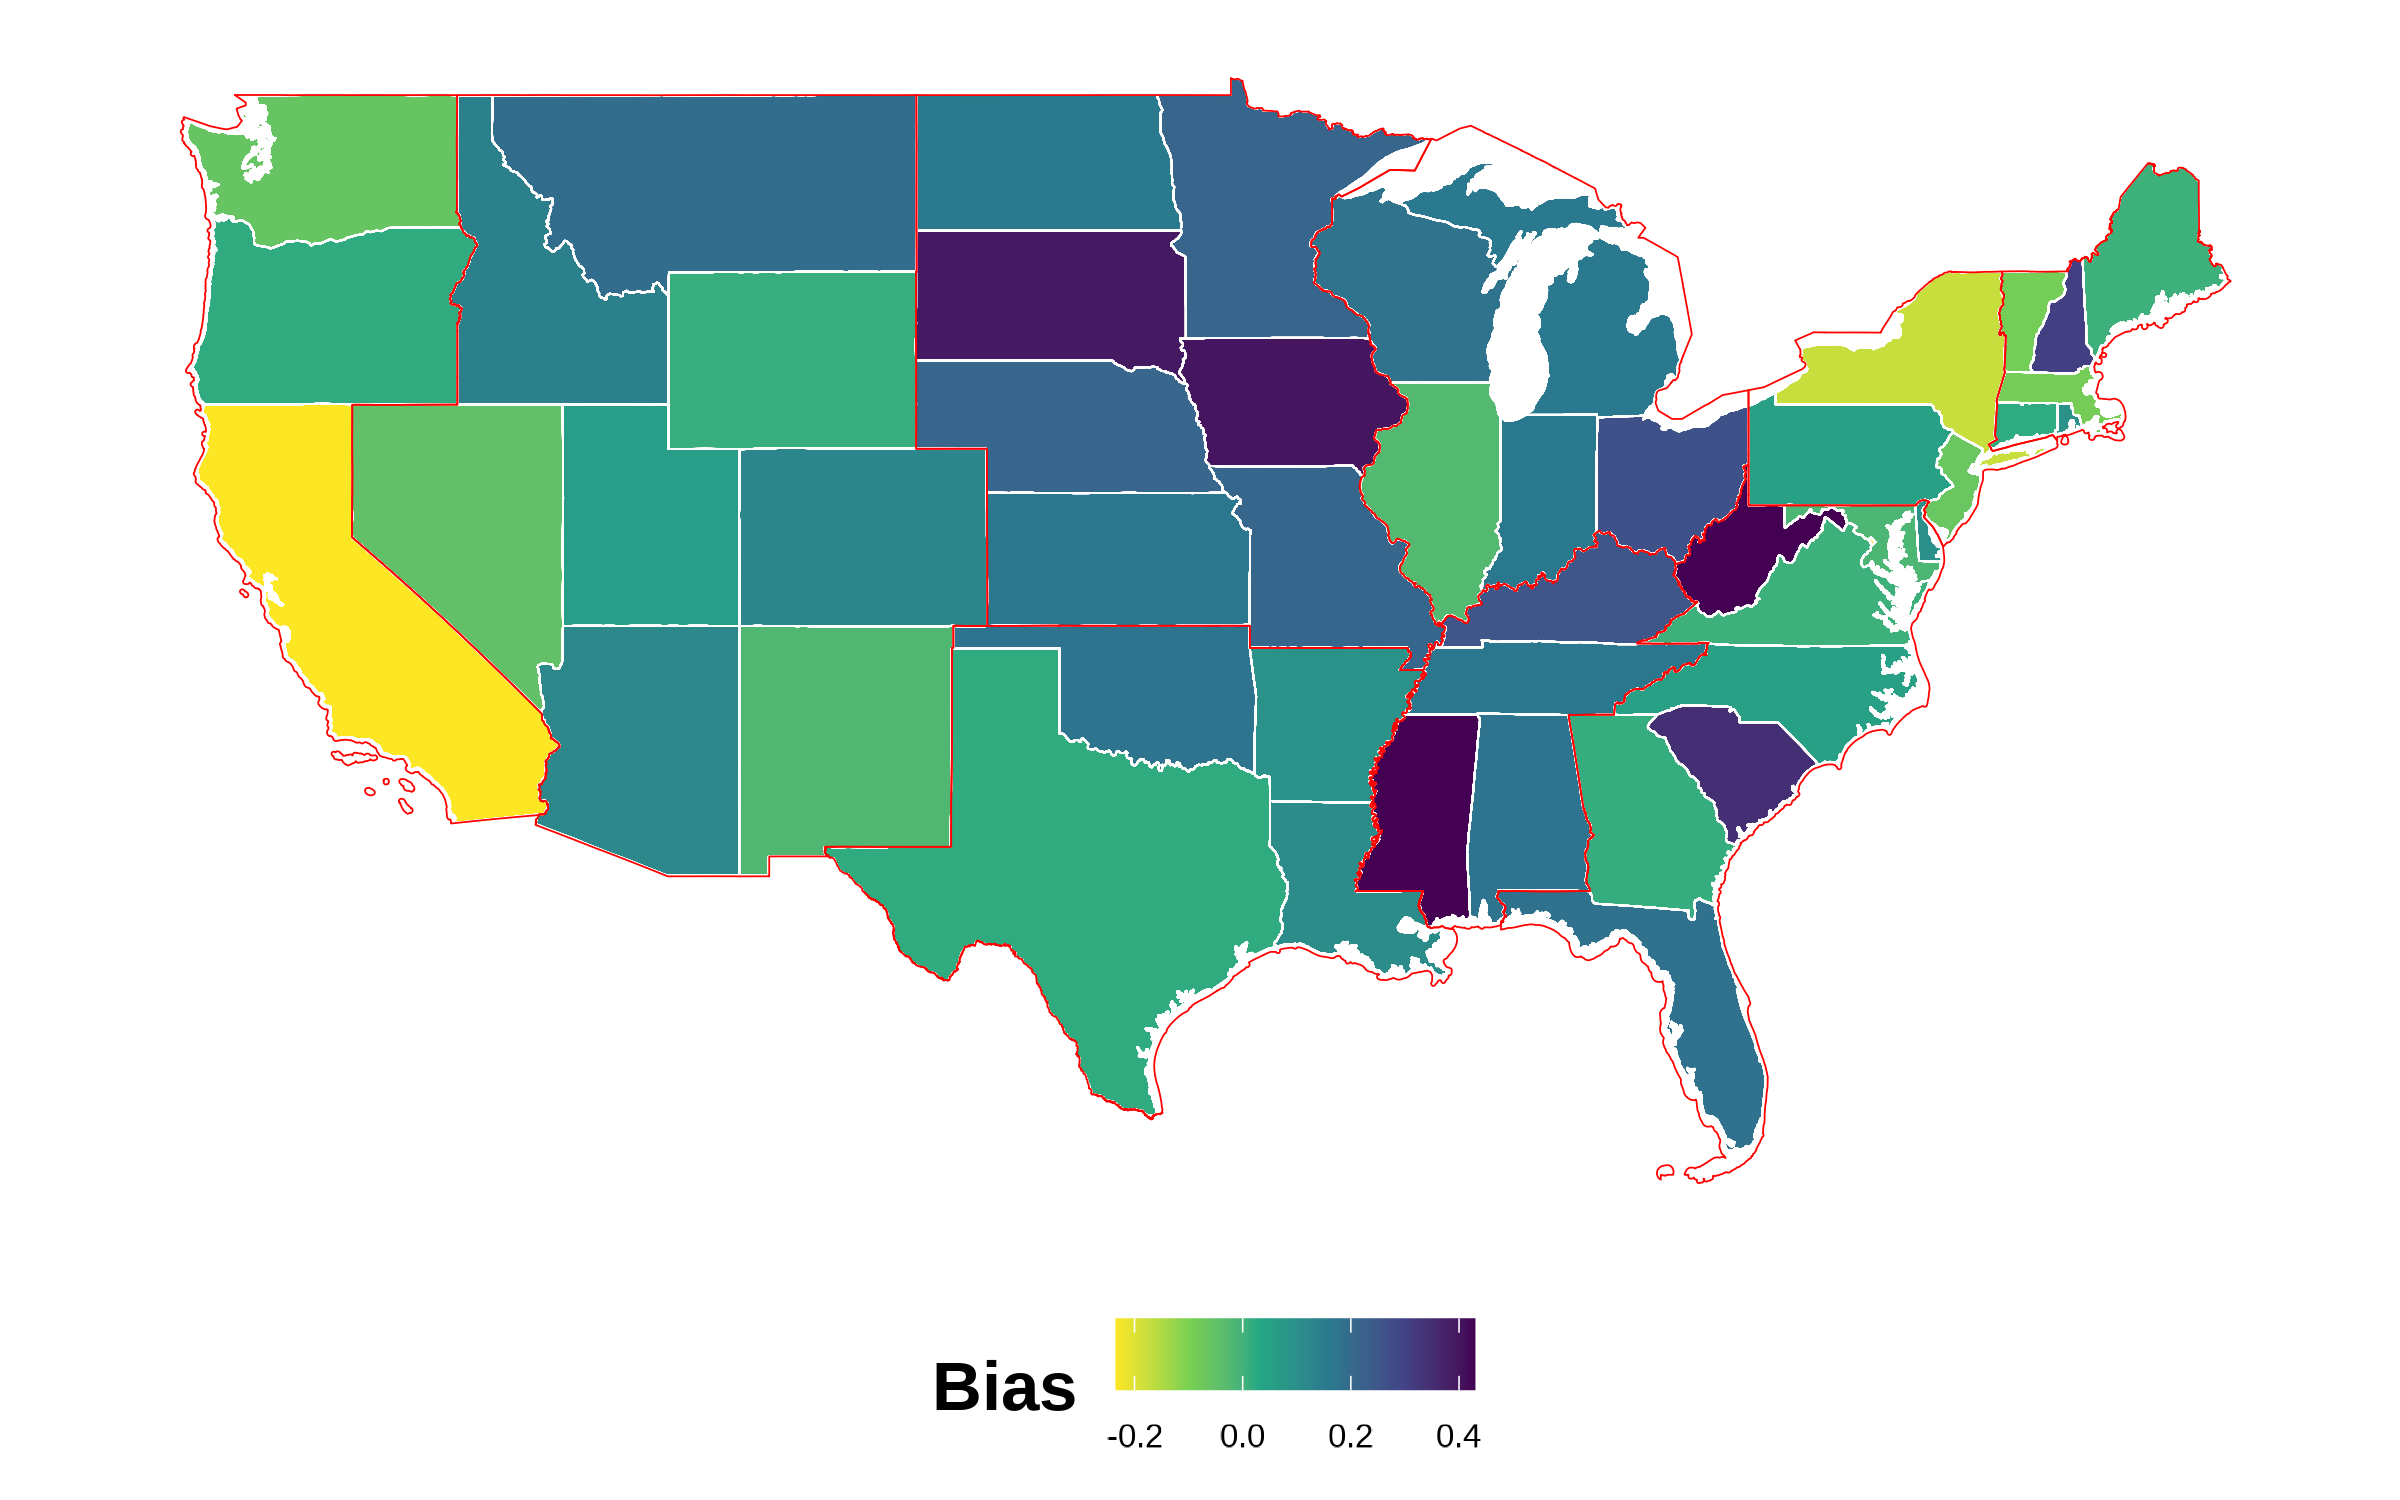
\includegraphics[width=0.9\linewidth]{figure/2016skinmap.png} 
\label{fig:skiniat-map-2016}
\end{subfigure}
\hfill%
% eigth
\begin{subfigure}{.45\textwidth}
\hspace{1cm}
\caption{State-level Bias in 2018}
\centering
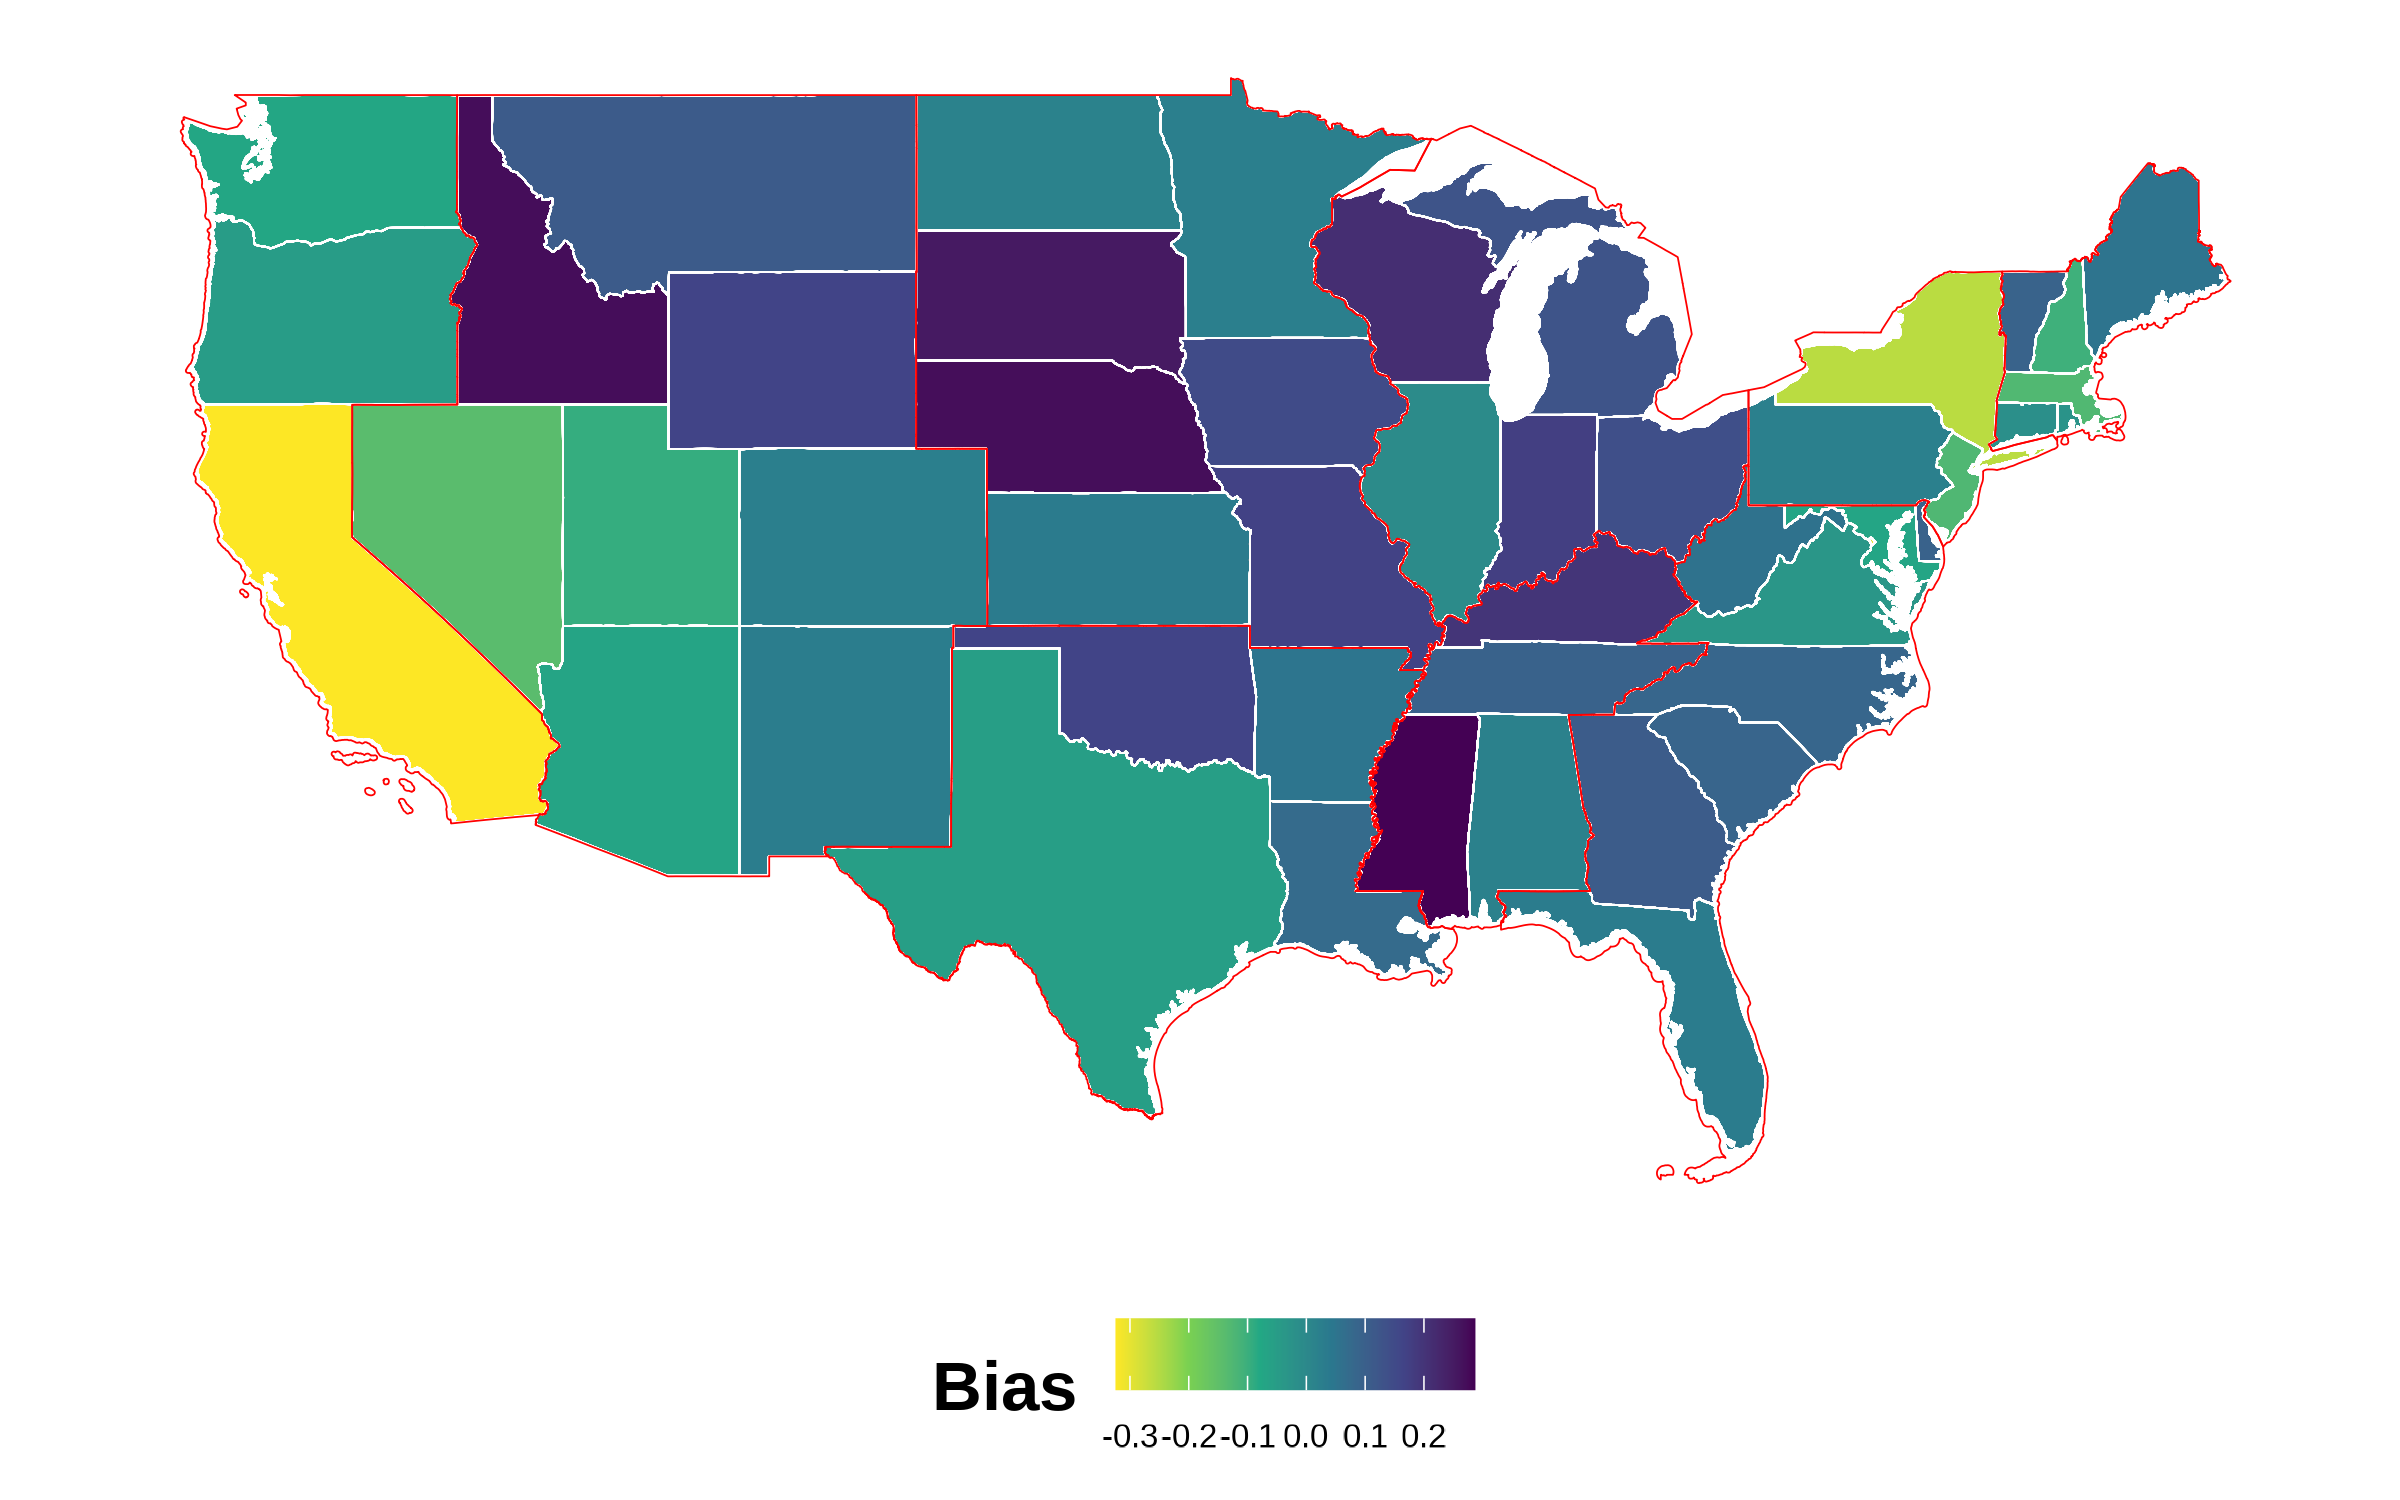
\includegraphics[width=0.9\linewidth]{figure/2018skinmap.png} 
\label{fig:skiniat-map-2018}
\hfill%
\end{subfigure}
\flushleft\footnotesize{\note{In this figure, I show the state-level implicit bias in different years in the sample. Each panel presents state-level bias during a certain year. The boundaries in red represent the different Census divisions in the United States. Notice how there is a variation across states with-in a region.}}
\end{figure}
\end{center}

\newpage
\pagebreak

\begin{center}
\begin{figure}[H]
\caption{Maps of State-level Implicit Association Test Bias 2004-2021 Measure with Census Division Regional Boundaries}
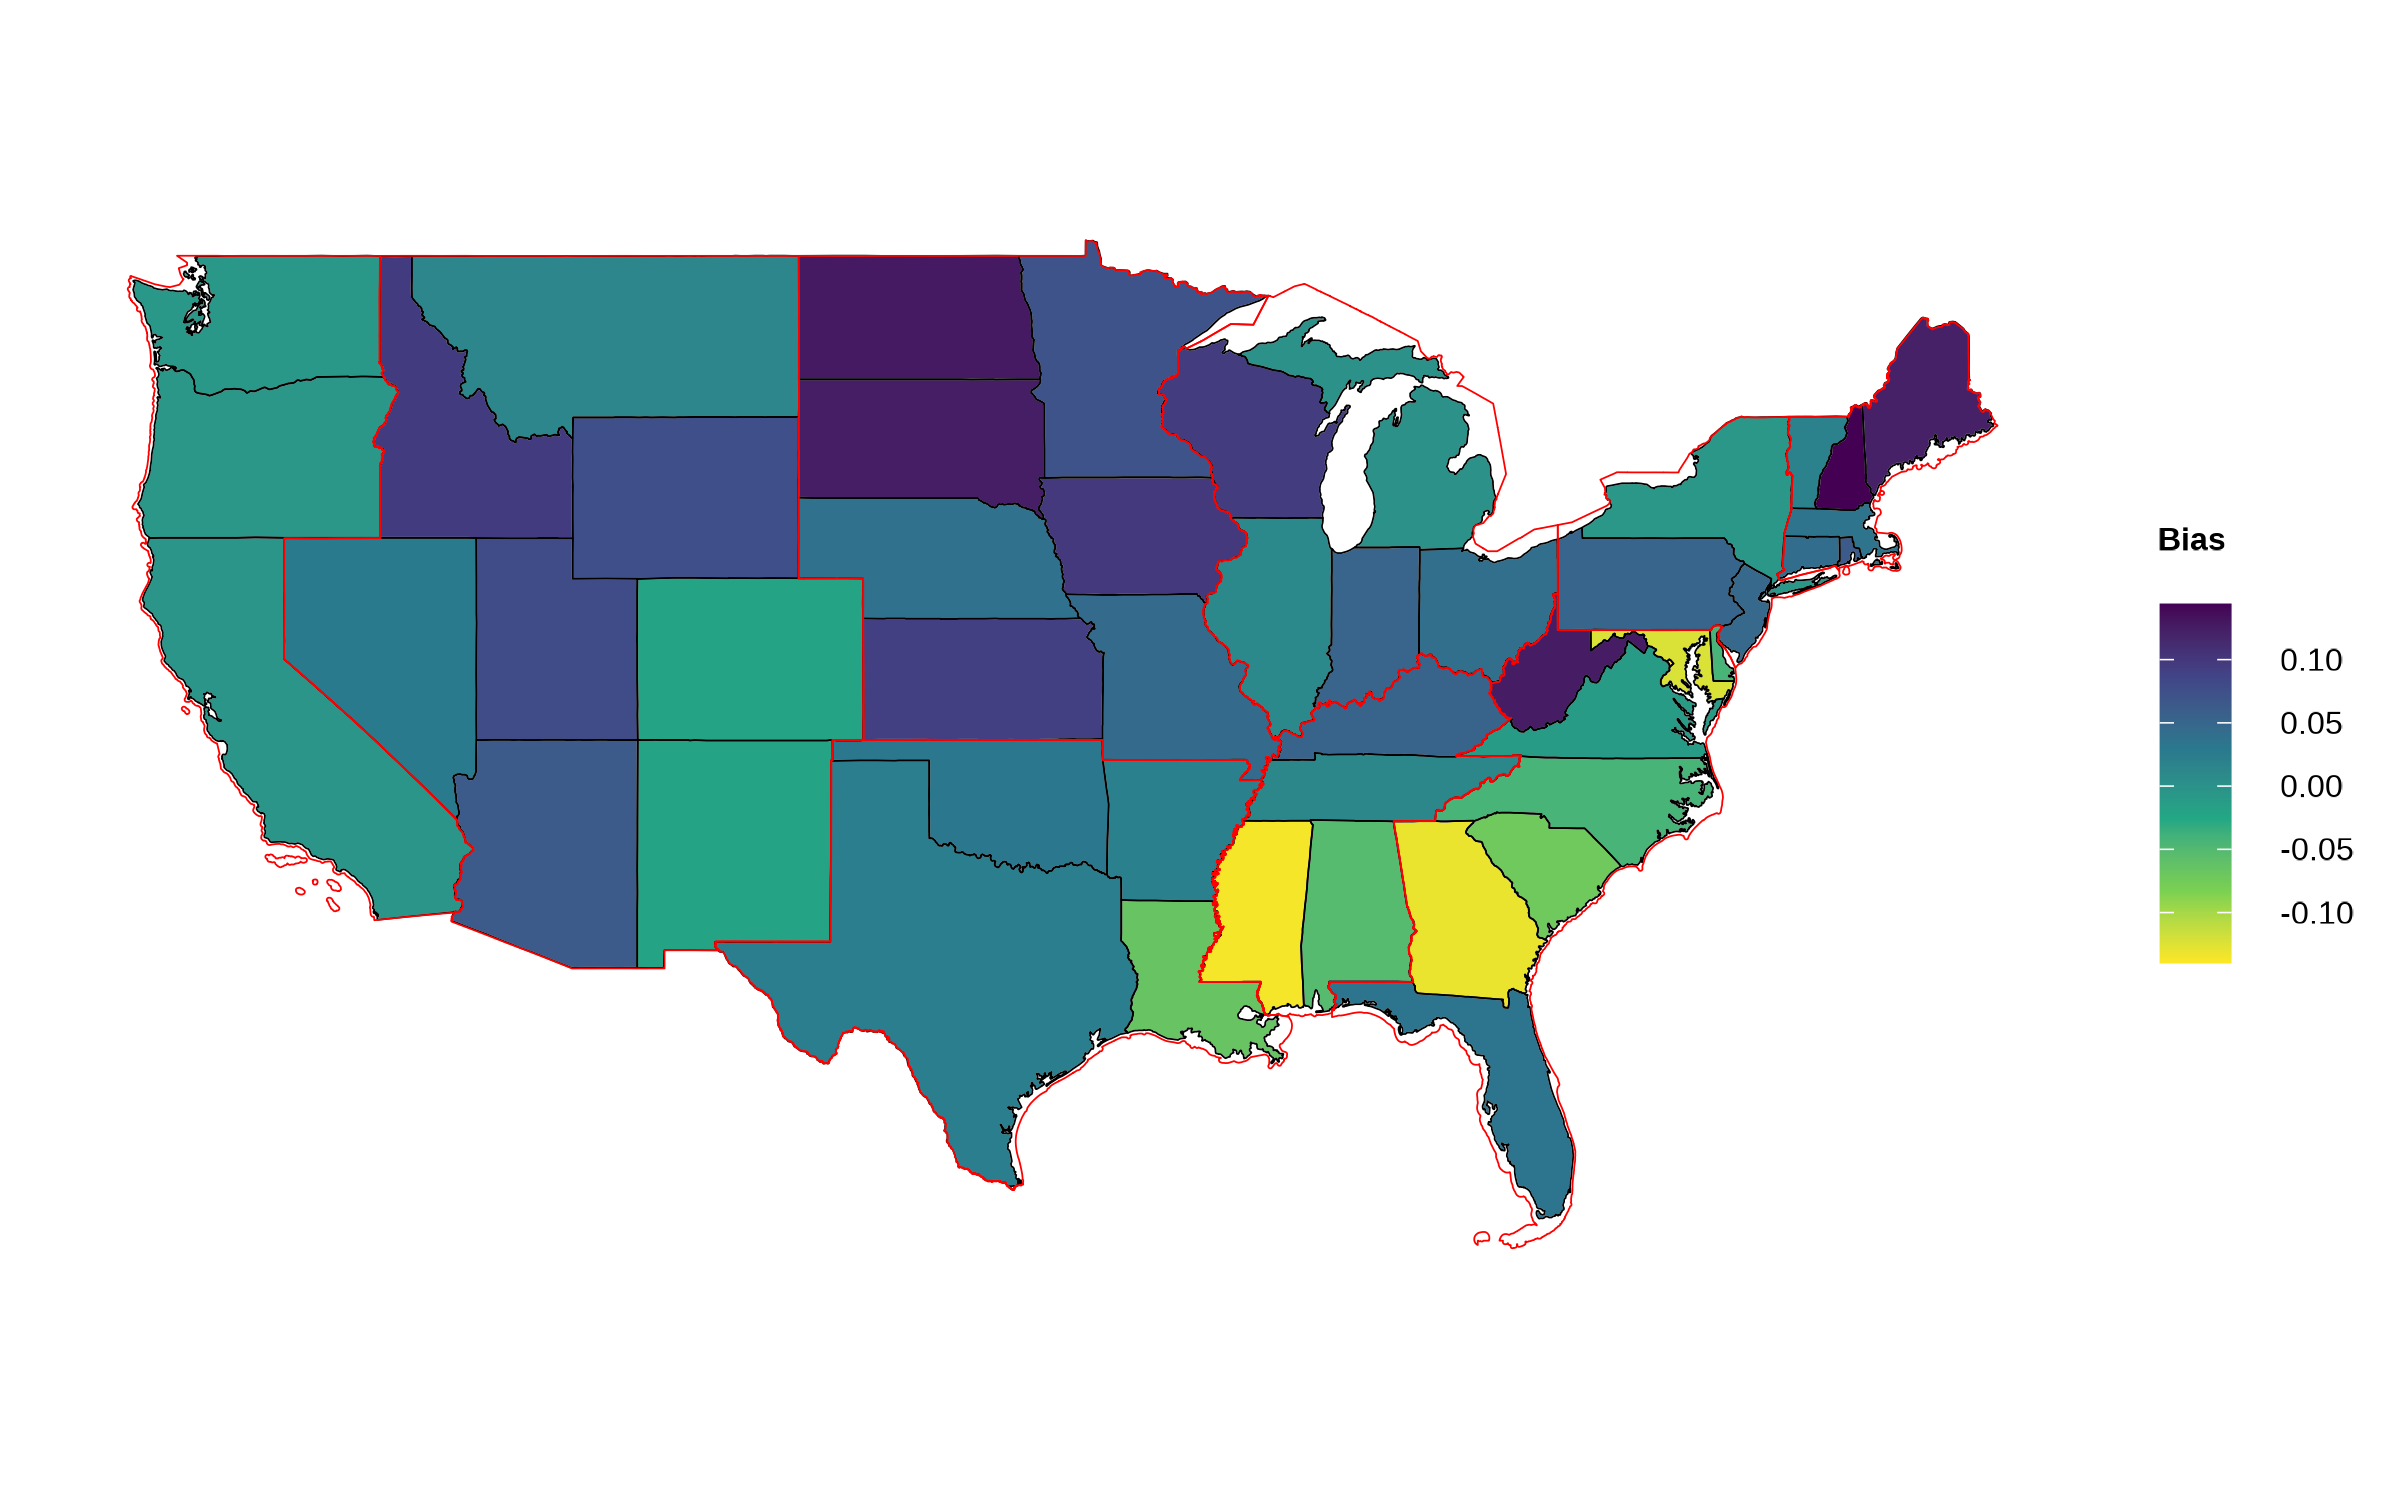
\includegraphics[width=\textwidth]{figure/skinmap_all.png} 
\label{fig:iat-map-all}
\flushleft\footnotesize{\note{In this figure, I show the state-level implicit bias in the sample of IAT tests from 2004 to 2021. The boundaries in red represent the different Census divisions in the United States. Notice how there is a variation across states with-in a region.}}
\end{figure}
\end{center}

\subsection{Measuring Prejudice}

The implicit association test measures how people associate concepts---for example, Black and dark-skinned people---and evaluations---good, bad. Respondents are asked to quickly match words into categories shown on a screen. Figure (\ref{fig:iatexamples}) shows a few examples of what a test taker would see on a skin tone implicit association test by Harvard's Project Implicit.

I use skin tone implicit association test data to construct a measure of state-level prejudice \citep{greenwaldMeasuringIndividualDifferences1998}. This measure has been used in the social sciences, especially in psychology. Previous work has shown that IAT test scores are hard to manipulate \citep{egloffPredictiveValidityImplicit2002}. \footnote{Research showed that the IAT tests are correlated with economic outcomes \citep{chettyRaceEconomicOpportunity2020,gloverDiscriminationSelfFulfillingProphecy2017}, voting behavior \citep{friesePredictingVotingBehavior2007}, and health \citep{leitnerRacialBiasAssociated2016}. Participation in the IAT, an online test, is voluntary. Therefore, the samples are not random and might suffer from selection bias in who decides to take the exam. However,  bias reflected by Implicit Association Test (IAT) scores as a way to measure prejudiced attitudes has been used as a proxy for prejudiced attitudes in an area \citet{chettyRaceEconomicOpportunity2020}.} Figure (\ref{fig:skiniat}) shows a graphical representation of the bias measure over time in the most and least biased places. A lower score implies less light-skin bias, whereas a higher score implies more discrimination against dark-skinned people. One-half of a standard deviation increase in bias is equivalent to the moving from Washington DC to North Dakota in 2012. I also show the state-level average bias over time in the maps in figure (\ref{fig:skiniat-maps}) and the overall average from 2004 to 2021 in figure (\ref{fig:iat-map-all}).


\section{Estimation and Results}\label{sec:empstrat}

Let $H_{ist}^g$ be the self-reported Hispanic identity of person $i$ in state $s$ at the time of interview $t$, let $Bias_{st}$ be the average state-level bias in state $s$ at time $t$, $DadCollegeGrad_{ist}$, and $MomCollegeGrad_{ist}$ are indicator variables that are equal to one if the father or mother graduated from college, $Women_{ist}$ is an indicator variable for sex, and $X_{ist}$ is a vector of controls.\footnote{The controls include quartic age, fraction of population that is Hispanic in state $s$, type of parents (WH, HW, or HH), type of grandparents (HHHH, HHHW, etc.), and dummy variables the generation to which person $i$ belong.} Additionally, $\gamma_{rt}$ is region-time fixed effects that controls for region $\times$ year specific shocks. The region $\times$ year also controls for systematic differences between regions in the overall Hispanic population, or bias toward Hispanics, even if they vary over time.

I first estimate if state-level bias is correlated with self-reported Hispanic identity. I estimate different specifications for each generation $g$. The basic equation I estimate is:
 
\begin{align}
H_{ist}^g &= \beta_1^g Bias_{st} + \beta_2^g DadCollegeGrad_{ist} + \beta_3^g MomCollegeGrad_{ist} \nonumber \\ 
			&+ \beta_4^g Women_{ist} + X_{ist}^g\pi + \gamma_{rt} 
           + \varepsilon_{ist}; 
           \text{where } g \in \{1,2,3\} \label{eq:identity_reg_bias}
\end{align}

I report the main results of estimating equation (\ref{eq:identity_reg_bias}) in figure (\ref{plot01-regression-gen}). I present the results of estimating the main specification on all three generations in panel (A) and on sub-samples of first-, second-, and third-generation immigrants in panels (B), (C), and (D) respectively. I find that bias and self-reported Hispanic identity are negatively associated, while parental education and self-reported Hispanic identity are positively associated. A one standard deviation increase in state-level bias is associated with an 11 percentage points decrease in self-reported Hispanic identity. Among first- and second-generation Hispanic immigrants, a one standard deviation increase in state-level bias is associated with 7 and 13 percentage points decrease in self-reported Hispanic identity.

I report the results of the same regression but on sub-samples of second-generation immigrants by type of parents---interethnic and endogamous parents---in figure (\ref{plot01-regression-byparent}). I present the results of estimating the main specification on second-generation immigrants in panel (A) and on sub-samples of HH, HW, and WH children in panels (B), (C), and (D), respectively. I find that children of endogamous Hispanic marriages are more influenced by state-level bias than those of interethnic marriages. I find that a one standard deviation increase in state-level bias is associated with 15 percentage points decrease in self-reported Hispanic identity among children of HH parents. 

I also report the results of the regression on sub-samples of third-generation immigrants by the number of Hispanic grandparents in table (\ref{regtab-bygrandparents}). I find that state-level bias is not significantly associated with the self-reported Hispanic identity of children of inter-ethnic grandparents. However, it is negatively associated with lower self-reported Hispanic identity of children of Hispanic grandparents. I find that a one standard deviation increase in state-level bias is associated with a 14 percentage points decrease in self-reported Hispanic identity.

\pagebreak
\newpage

\begin{center}
\begin{figure}[!htb]
\centering
\caption{Relationship Between Self-Reported Hispanic Identity and Bias: By Generation}
\label{plot01-regression-gen}
%First graph
\begin{subfigure}{.48\textwidth}
\caption{All Generations}
\centering
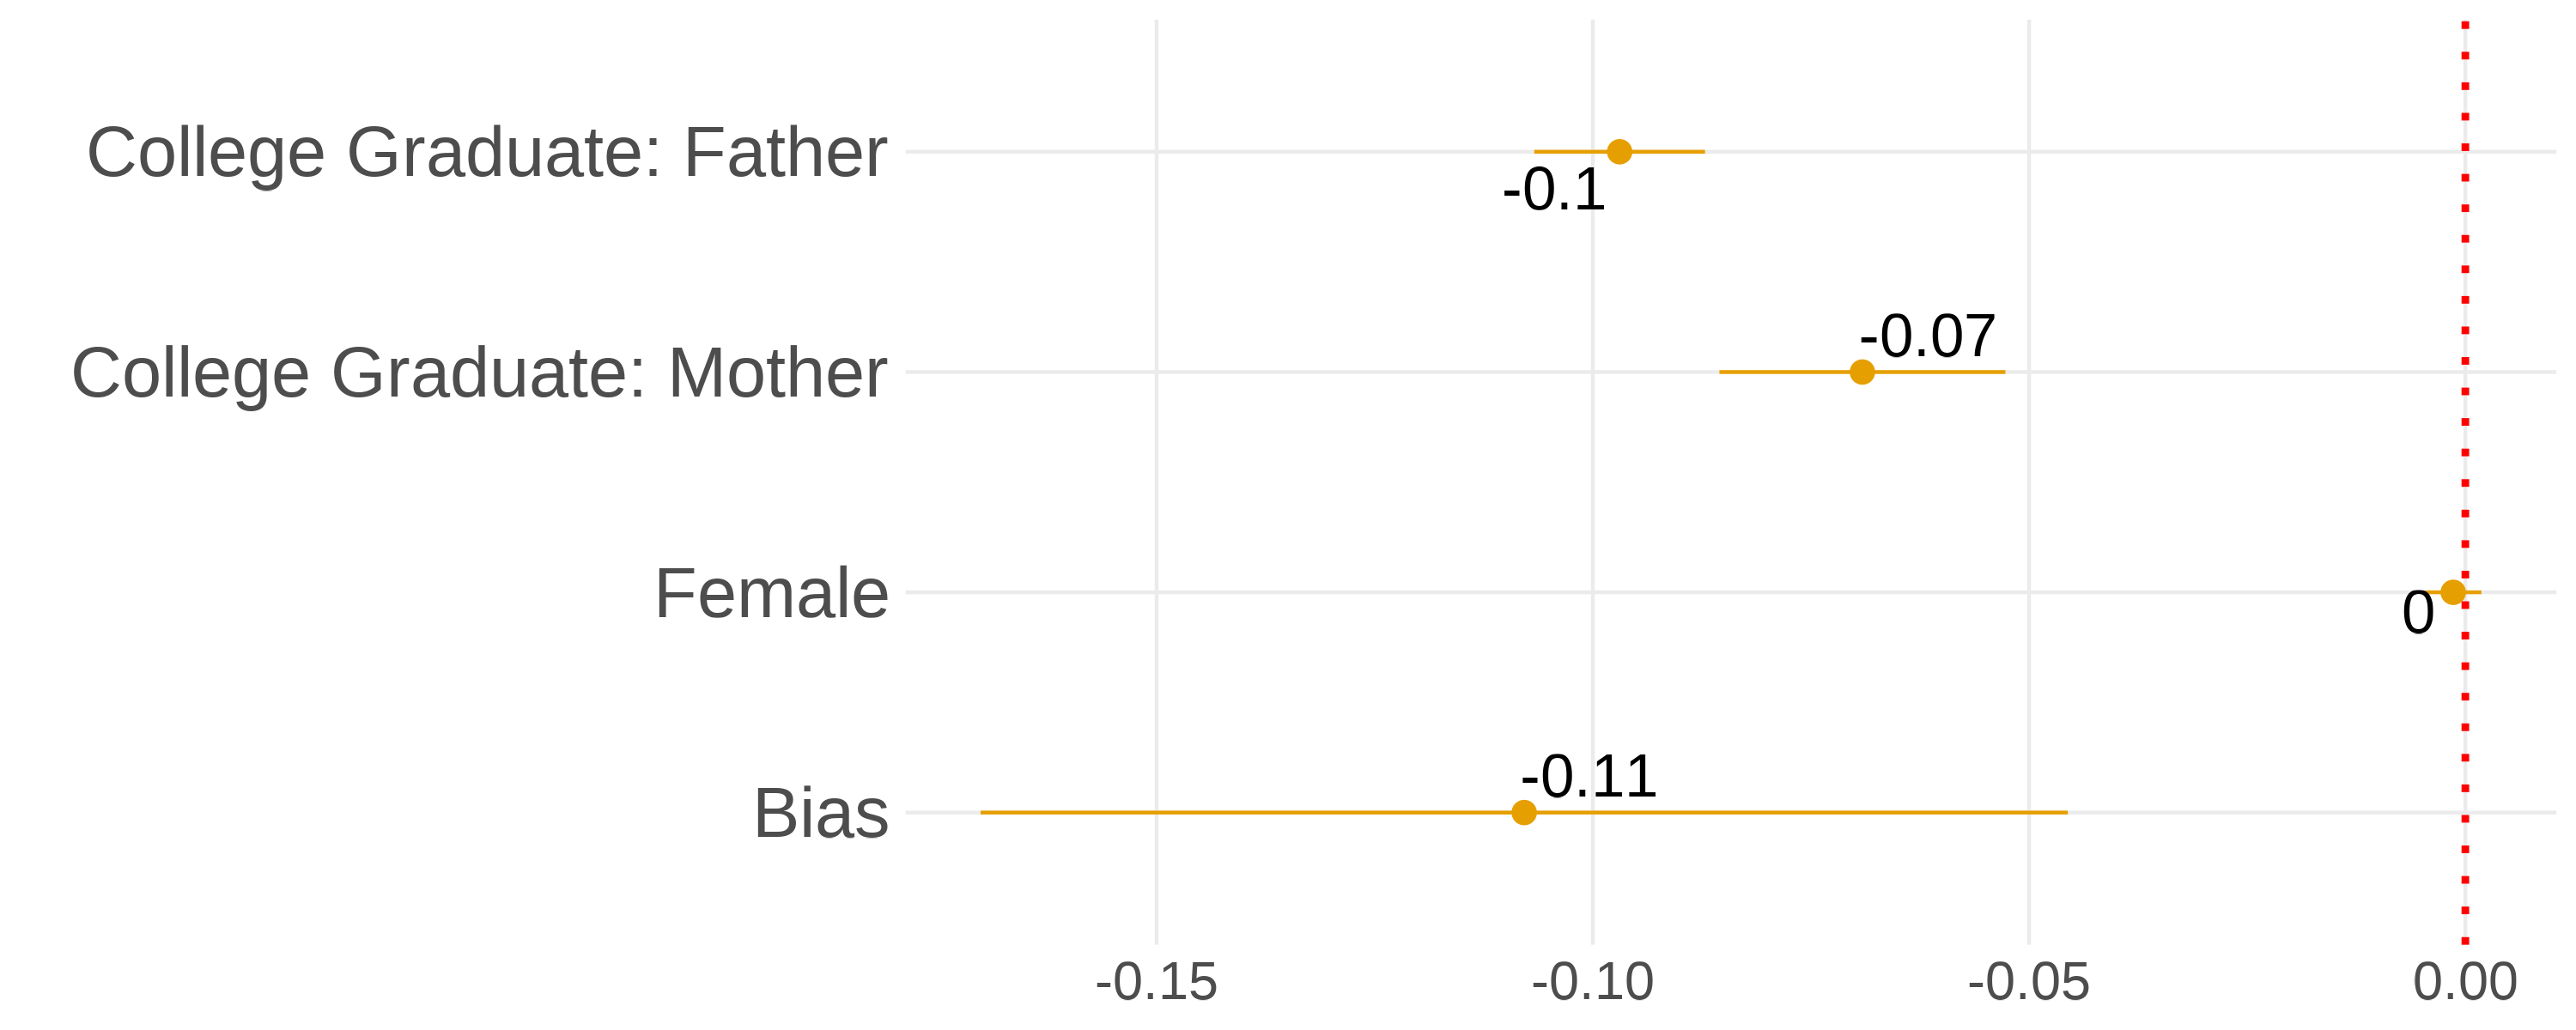
\includegraphics[width=.9\linewidth]{figure/skin-iat-regression-all-gens.png}
\end{subfigure}
\centering
%Second graph
\begin{subfigure}{.48\textwidth}
\caption{First-Generation}
\centering
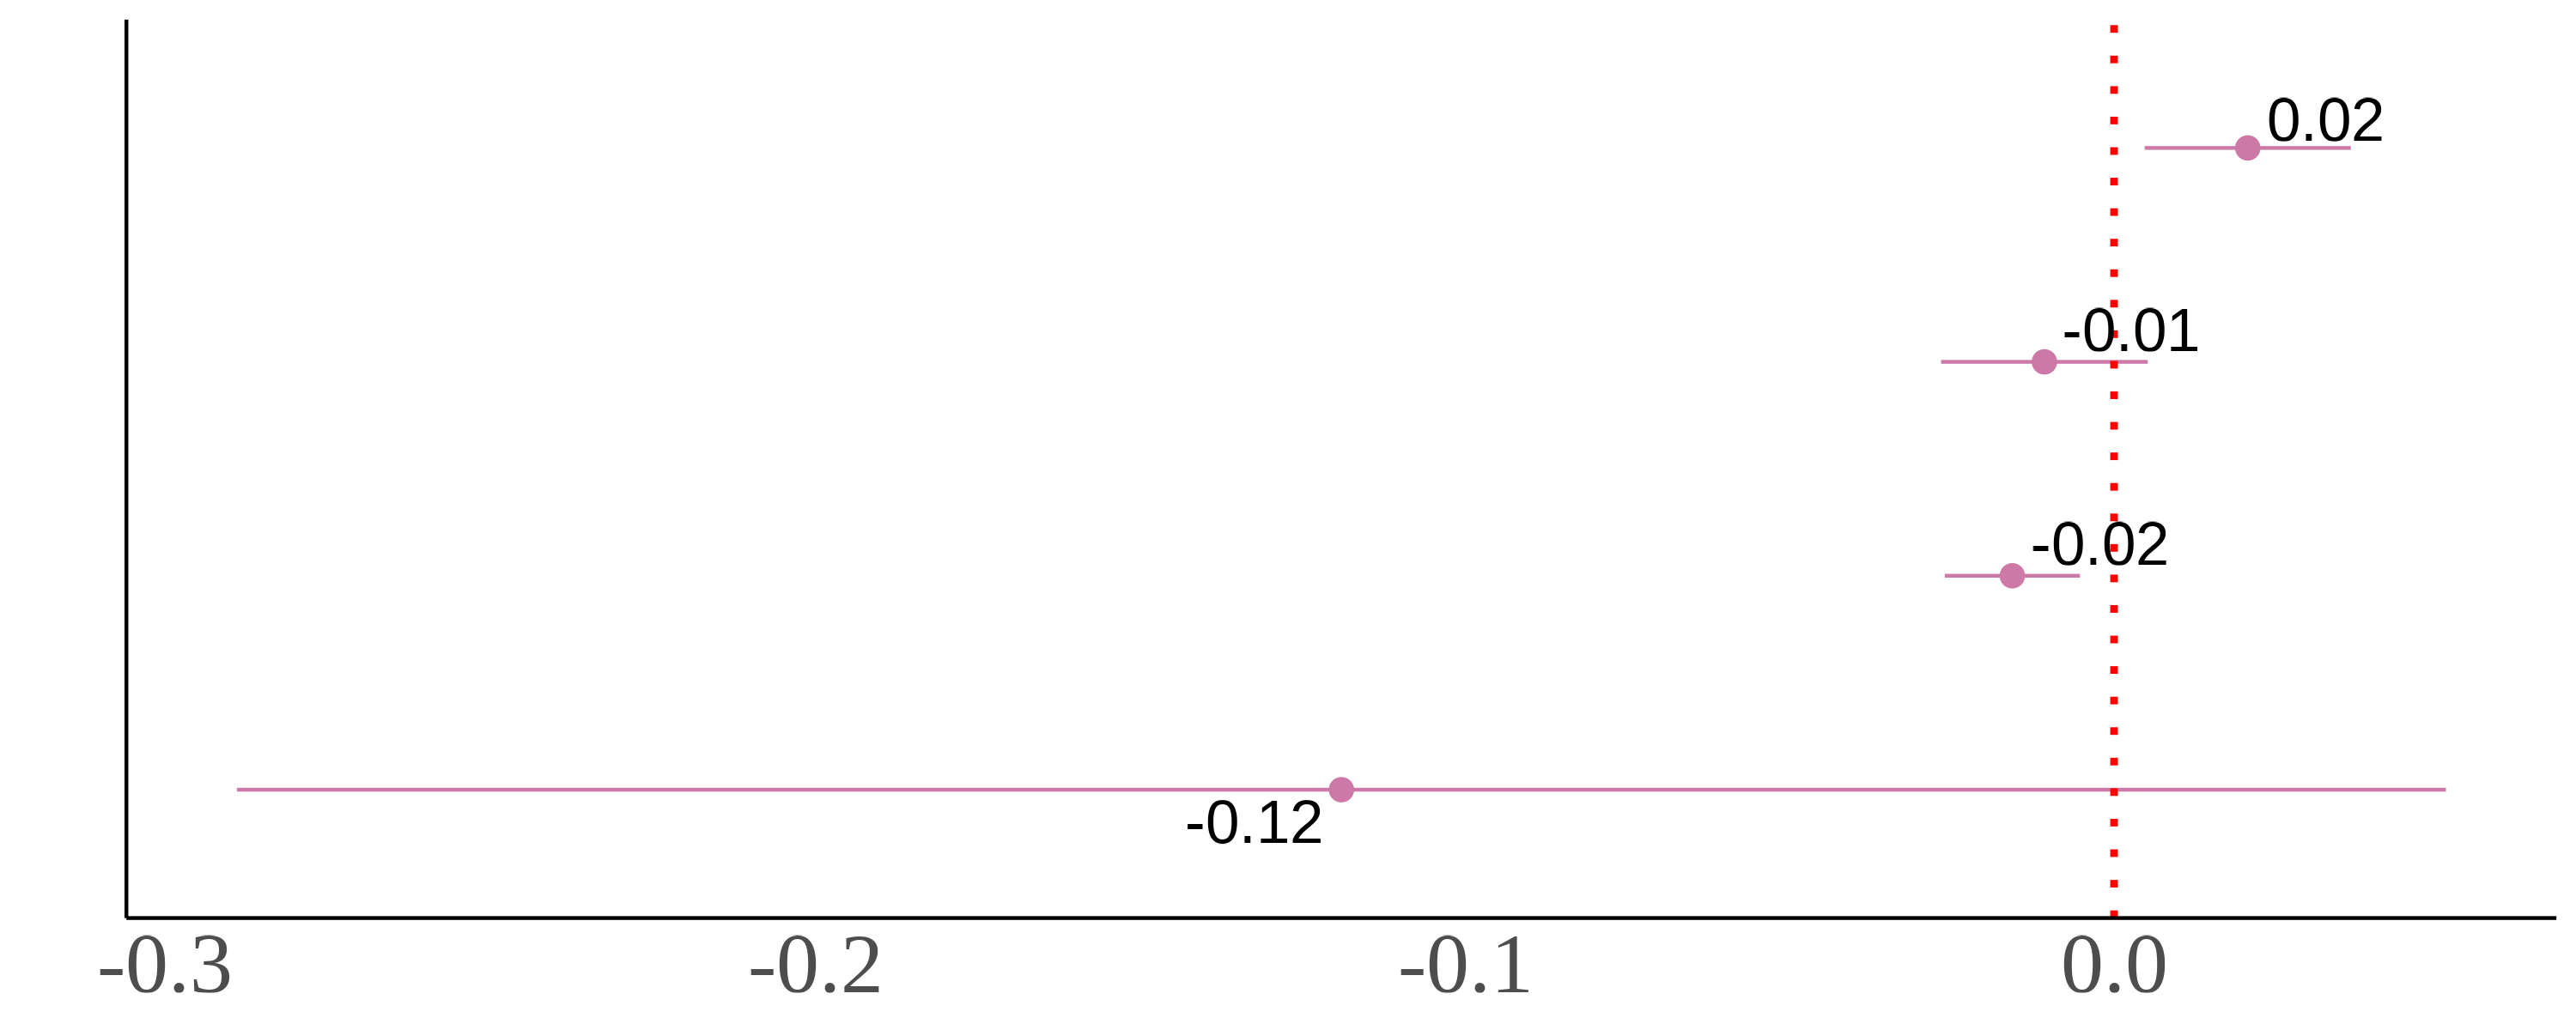
\includegraphics[width=.9\linewidth]{figure/skin-iat-regression-first-gen.png}
\end{subfigure}
%Third Graph
\begin{subfigure}{.48\textwidth}
\caption{Second-Generation}
\centering
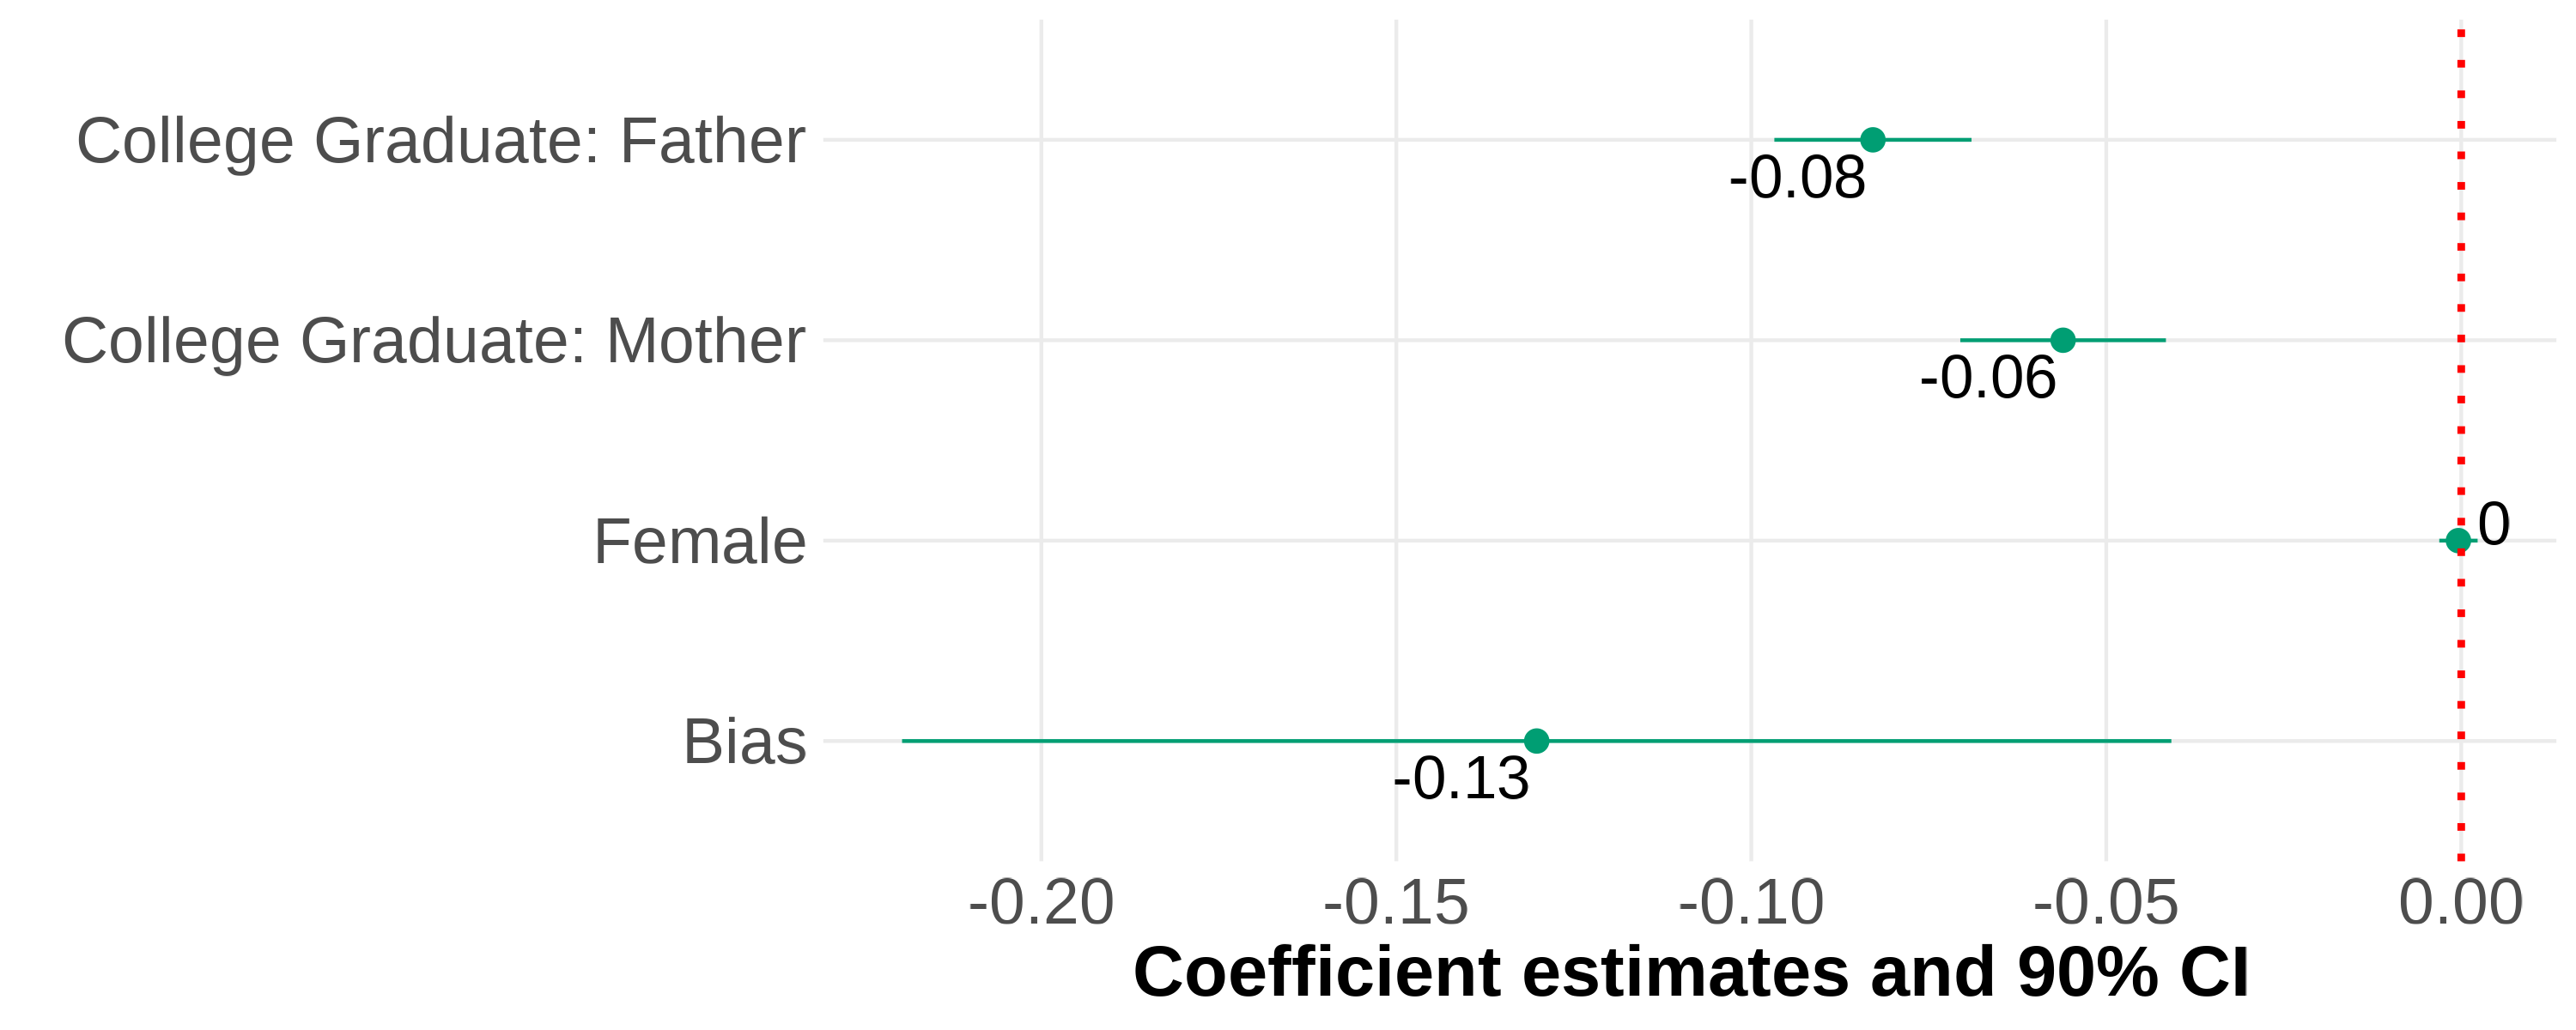
\includegraphics[width=.9\linewidth]{figure/skin-iat-regression-second-gen.png}
\end{subfigure}
%Fourth Graph
\begin{subfigure}{.48\textwidth}
\caption{Third-Generation}
\centering
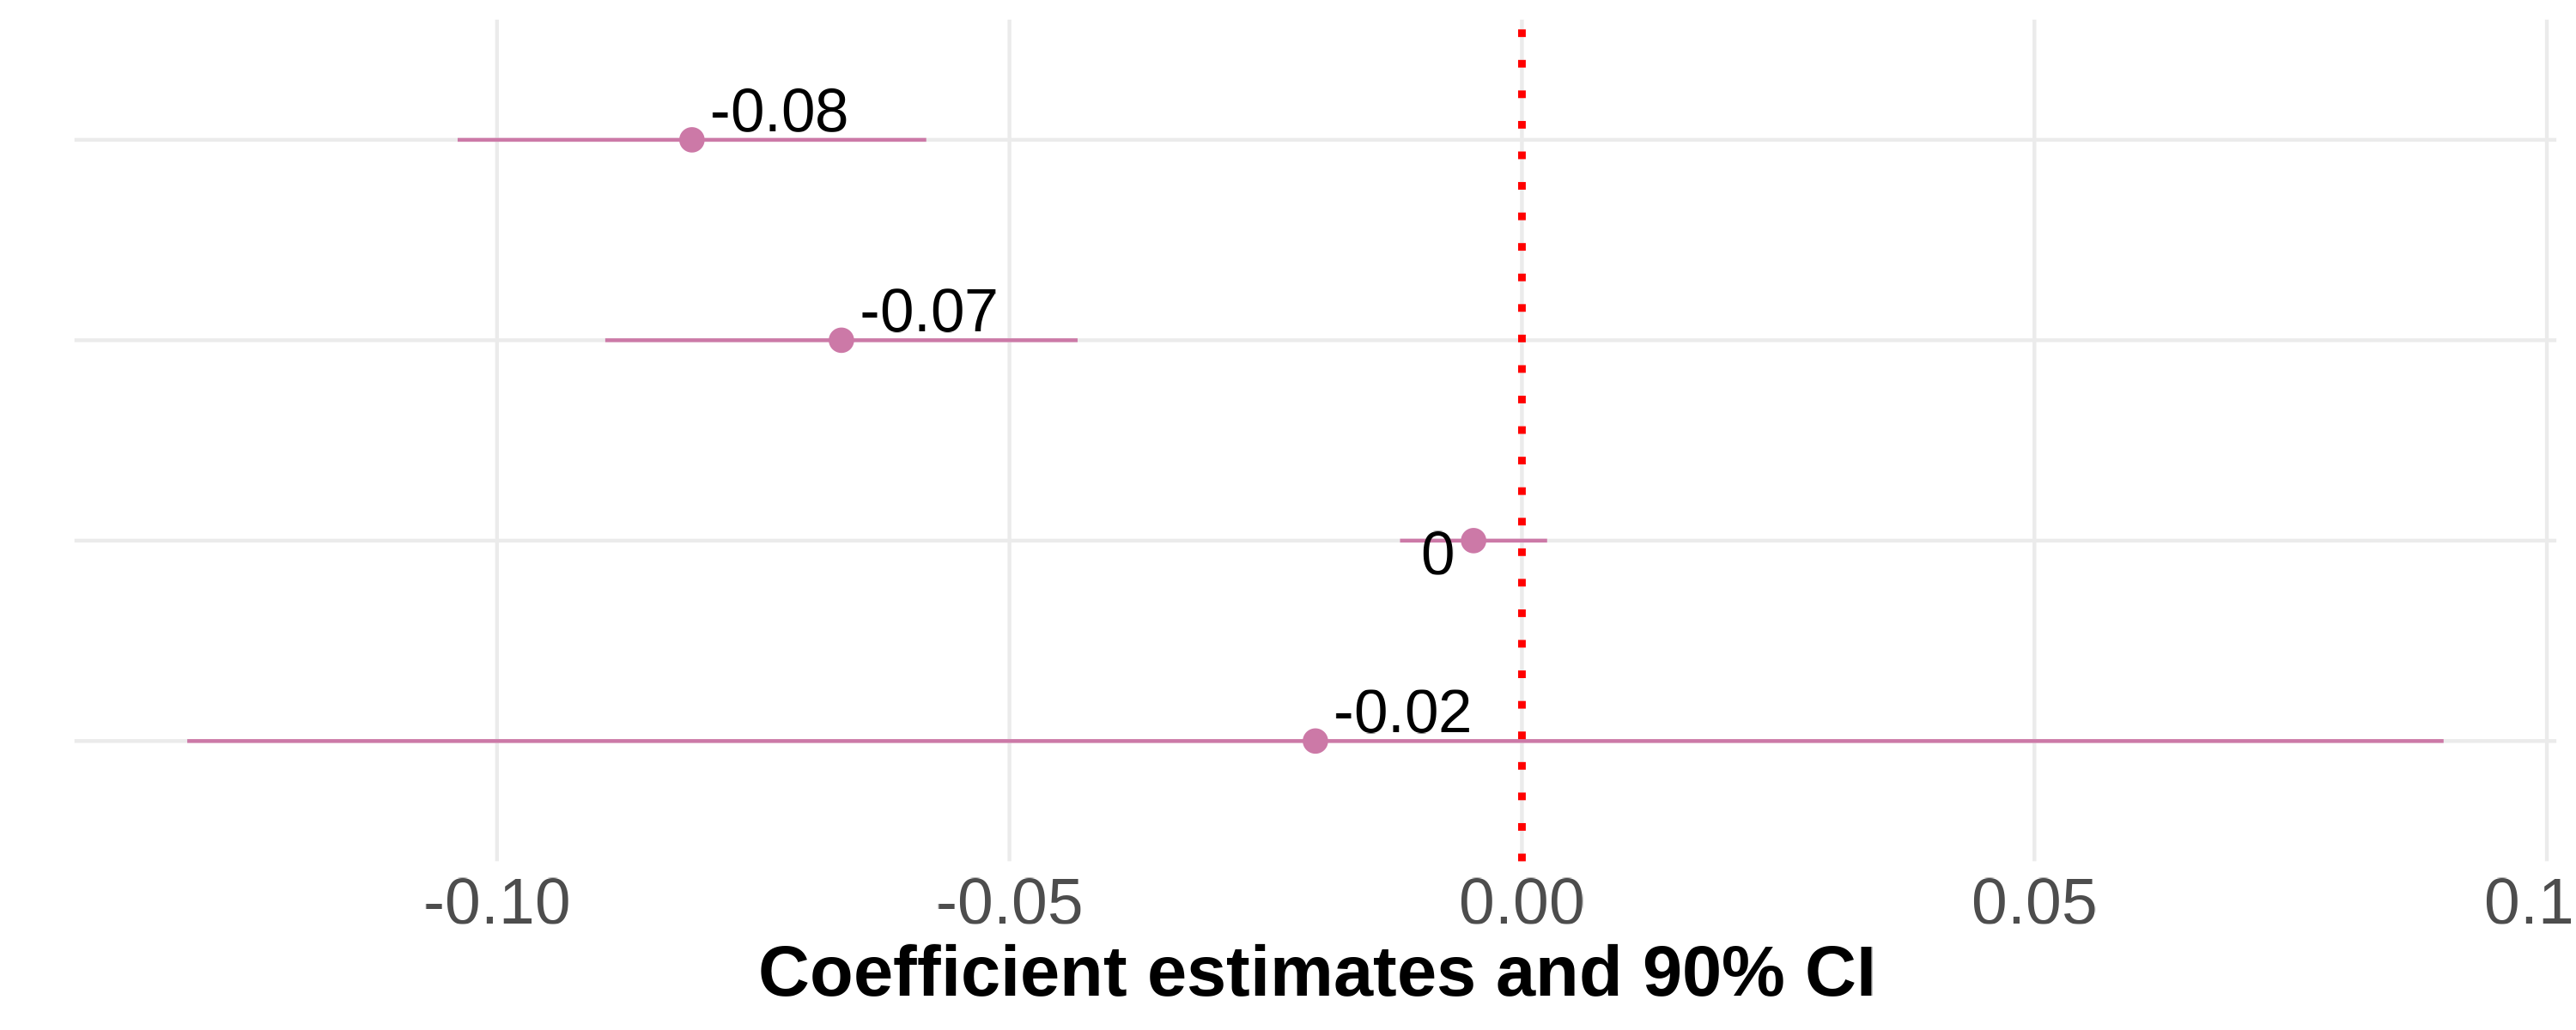
\includegraphics[width=.9\linewidth]{figure/skin-iat-regression-third-gen.png}
\end{subfigure}
\flushleft\footnotesize{\note{I show four panels of estimating equation (\ref{eq:identity_reg_bias}). I include region $\times$ year fixed effects with controls for sex, quartic age, and parental education. The dependent variable is self-reported Hispanic identity and the independent variable is state-level bias. Each panel is the results from the same regression but on different samples that are divided by generation. Standard errors are clustered on the state level. The samples include first-, second-, and third-generation Hispanic children ages 17 and below who live in intact families. First-generation Hispanic immigrants are children that were born in a Spanish-speaking county. Native-born second-generation Hispanic immigrants are children with at least one parent born in a Spanish-speaking country. Finally, native-born third-generation Hispanic immigrants are children with native-born parents and at least one grandparent born in a Spanish-speaking country.}}
\end{figure}
\end{center}

\pagebreak
\newpage

\begin{center}
\begin{figure}[!htb]
\centering
\caption{Relationship Between Self-Reported Hispanic Identity and Bias: By Parental Types}
\label{plot01-regression-byparent}
%First graph
\begin{subfigure}{.48\textwidth}
\caption{Second-Generation (All Parental Types)}
\centering
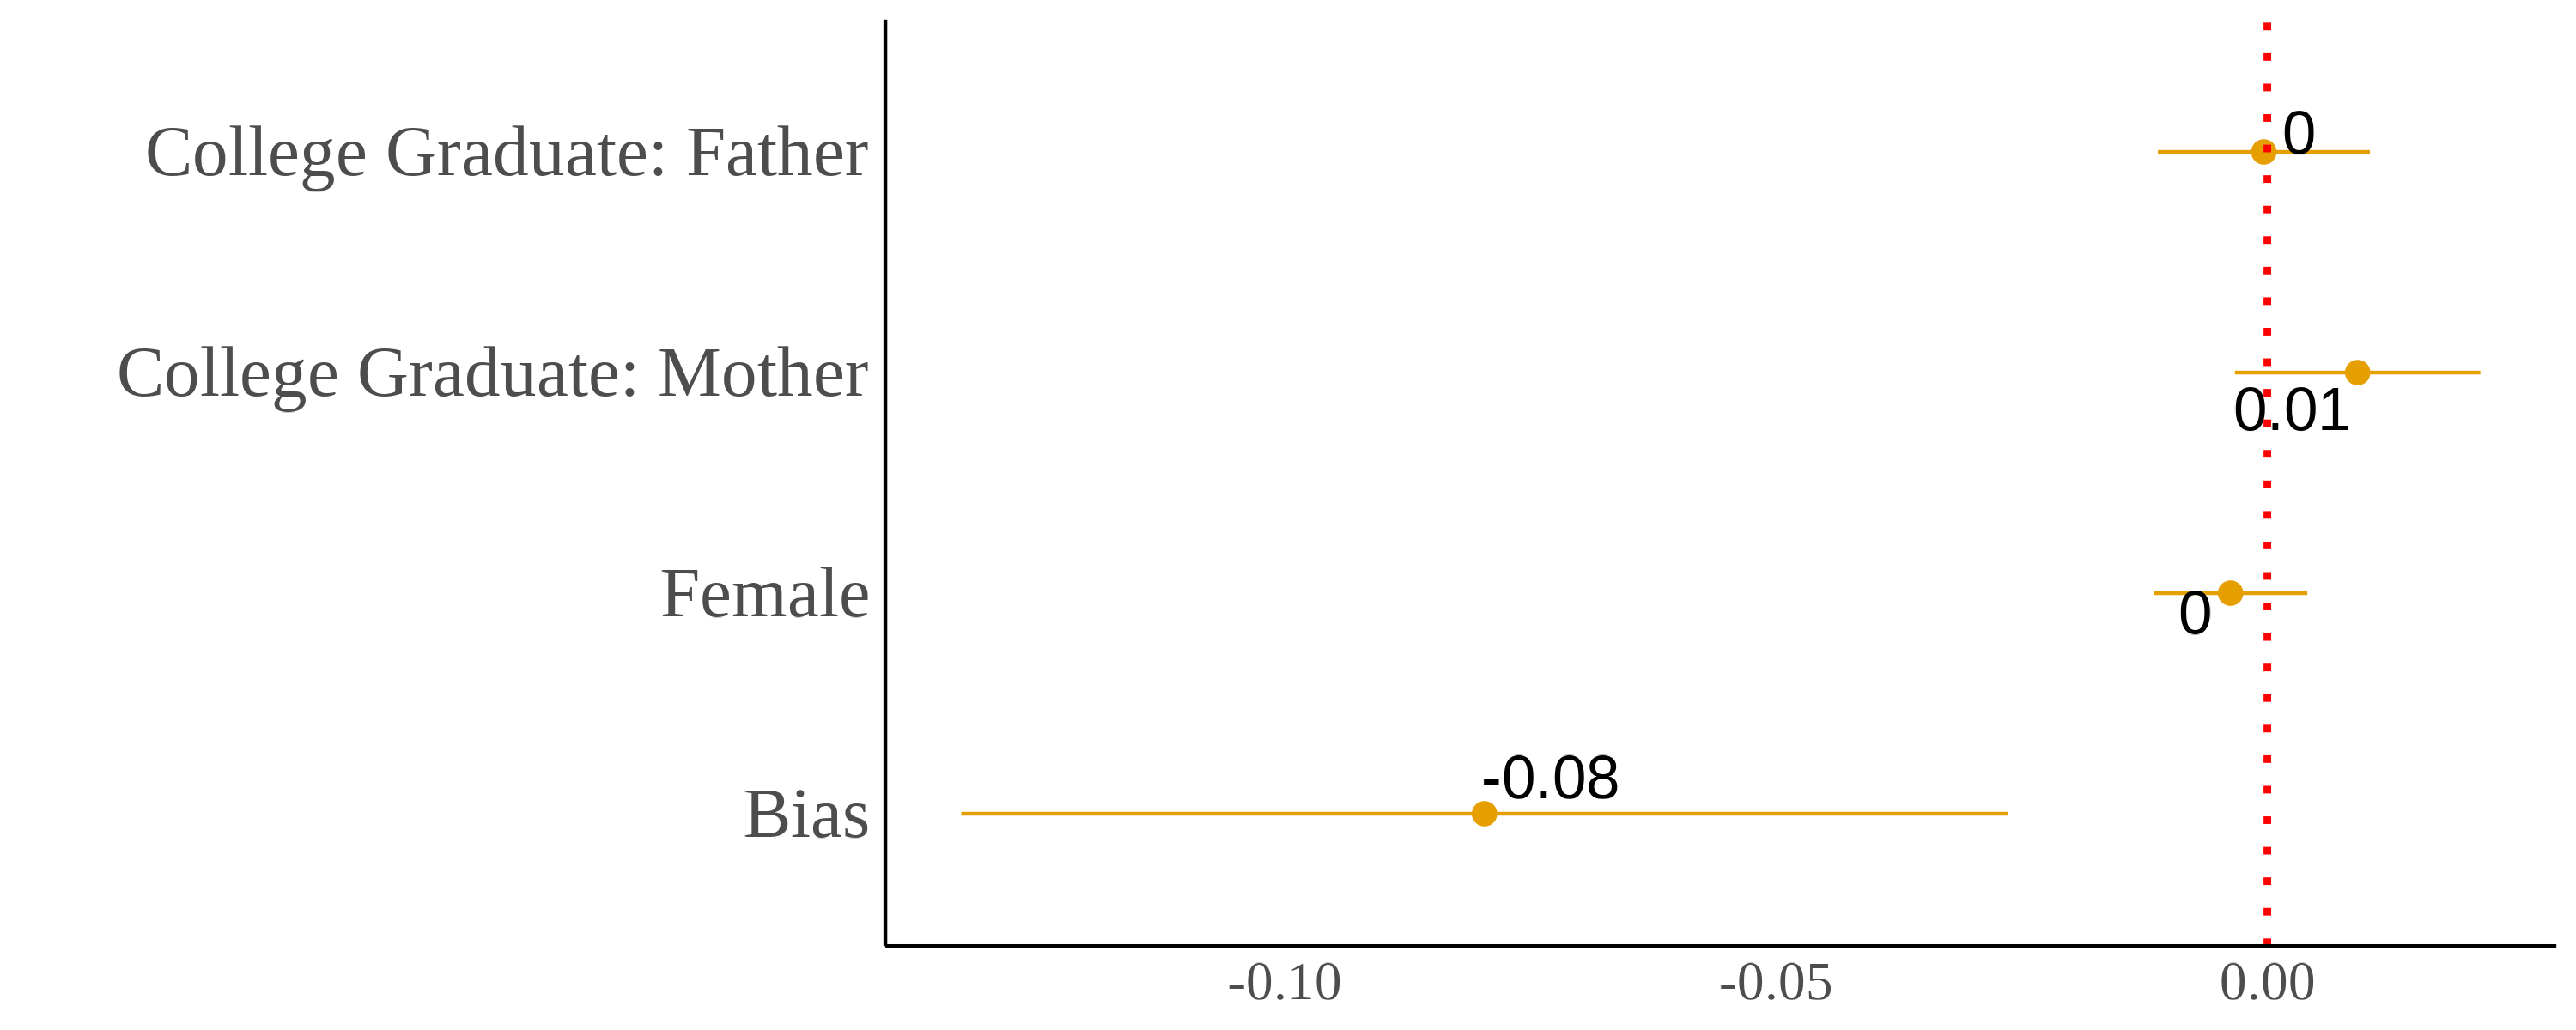
\includegraphics[width=.9\linewidth]{figure/by-parents-regs-all.png}
\end{subfigure}
\centering
%Second graph
\begin{subfigure}{.48\textwidth}
\caption{Hispanic Fathers-Hispanic Mothers}
\centering
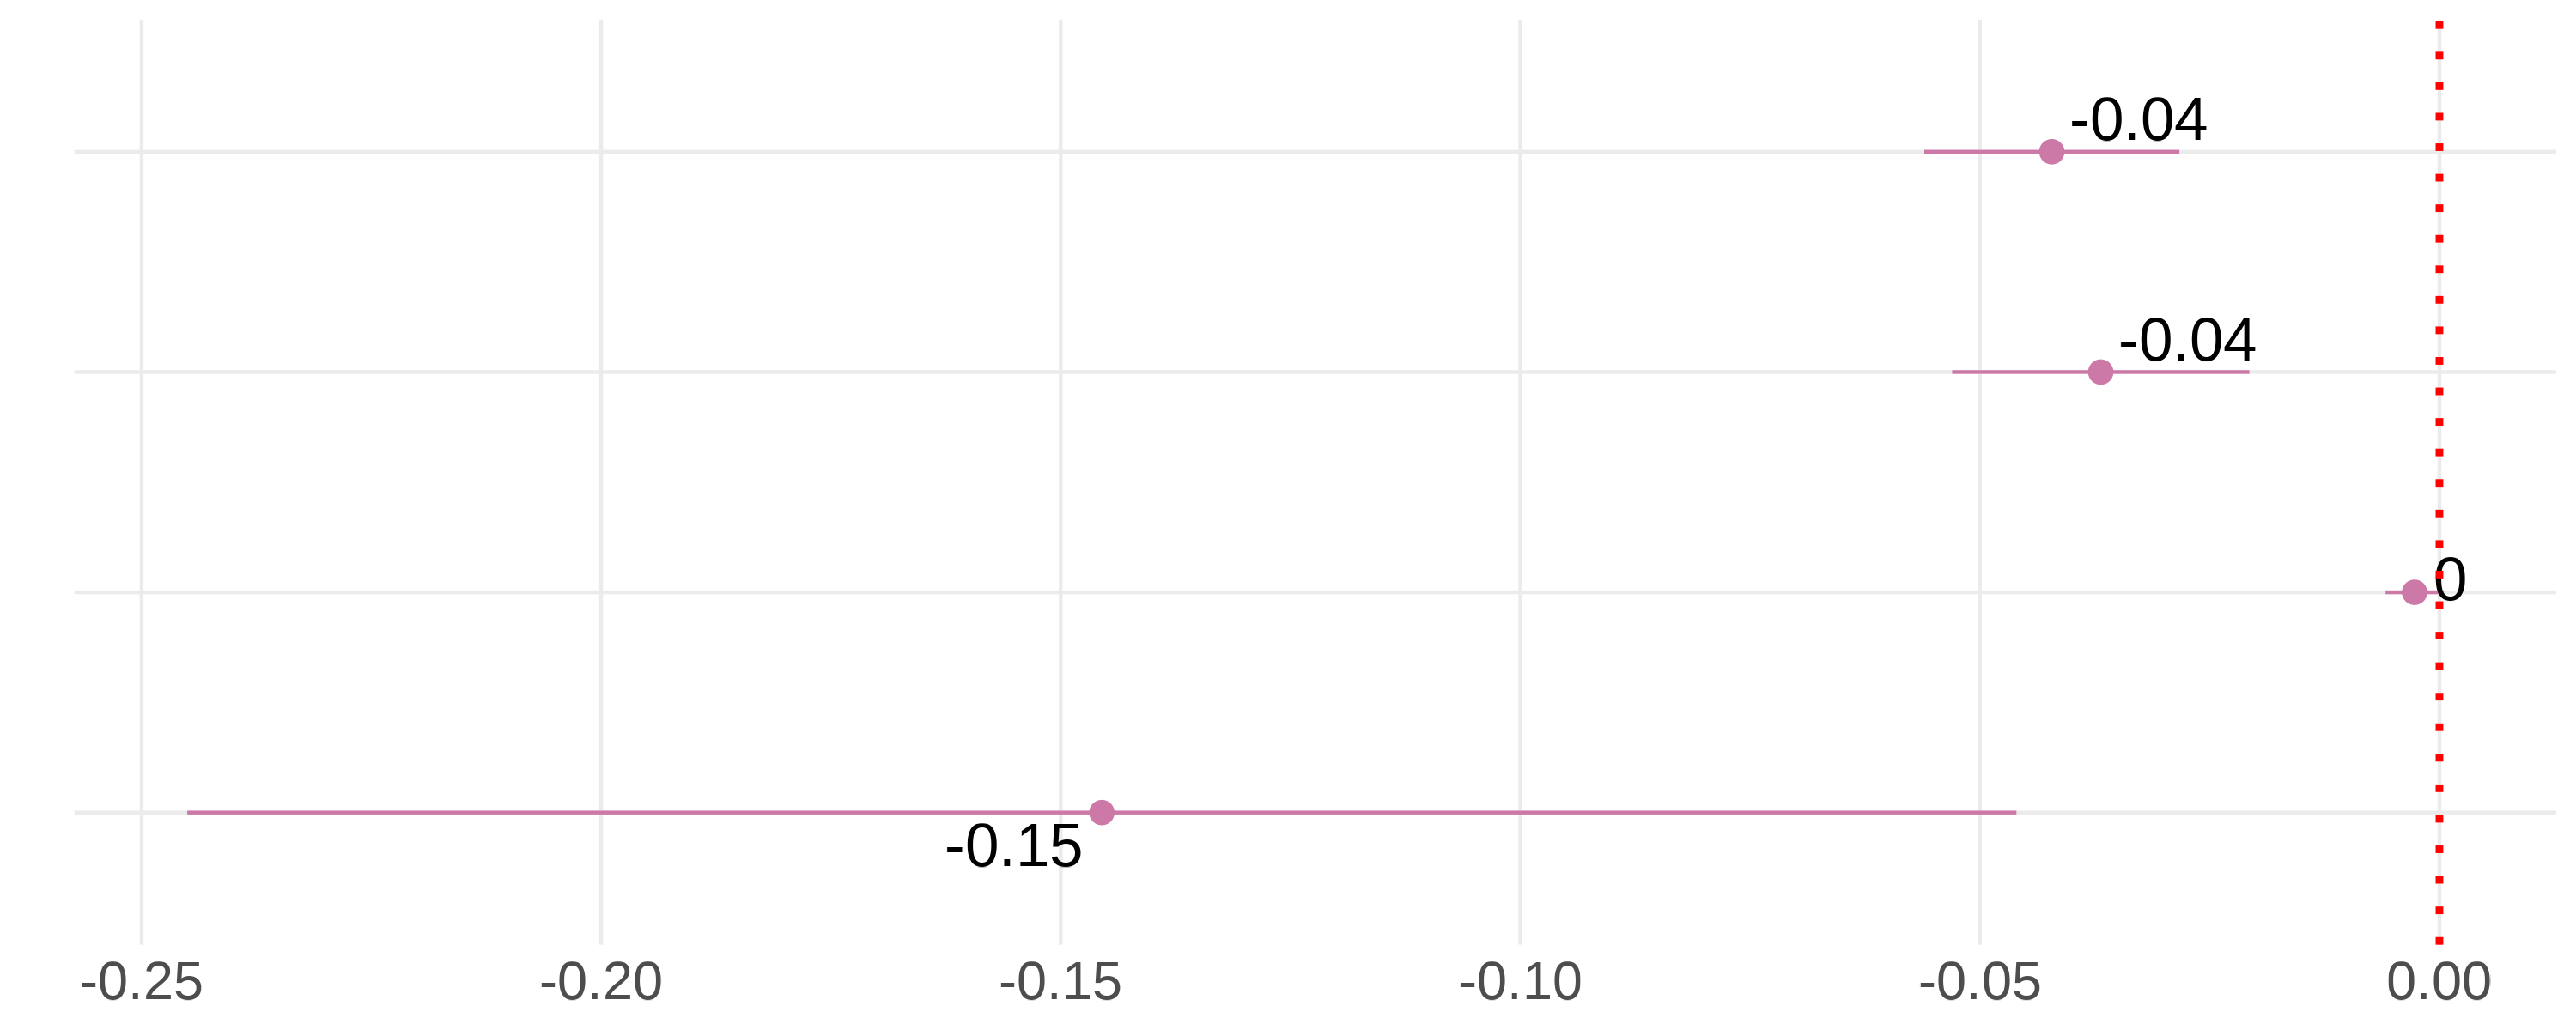
\includegraphics[width=.9\linewidth]{figure/by-parents-regs-hh.png}
\end{subfigure}
%Third Graph
\begin{subfigure}{.48\textwidth}
\caption{Hispanic Fathers-White Mothers}
\centering
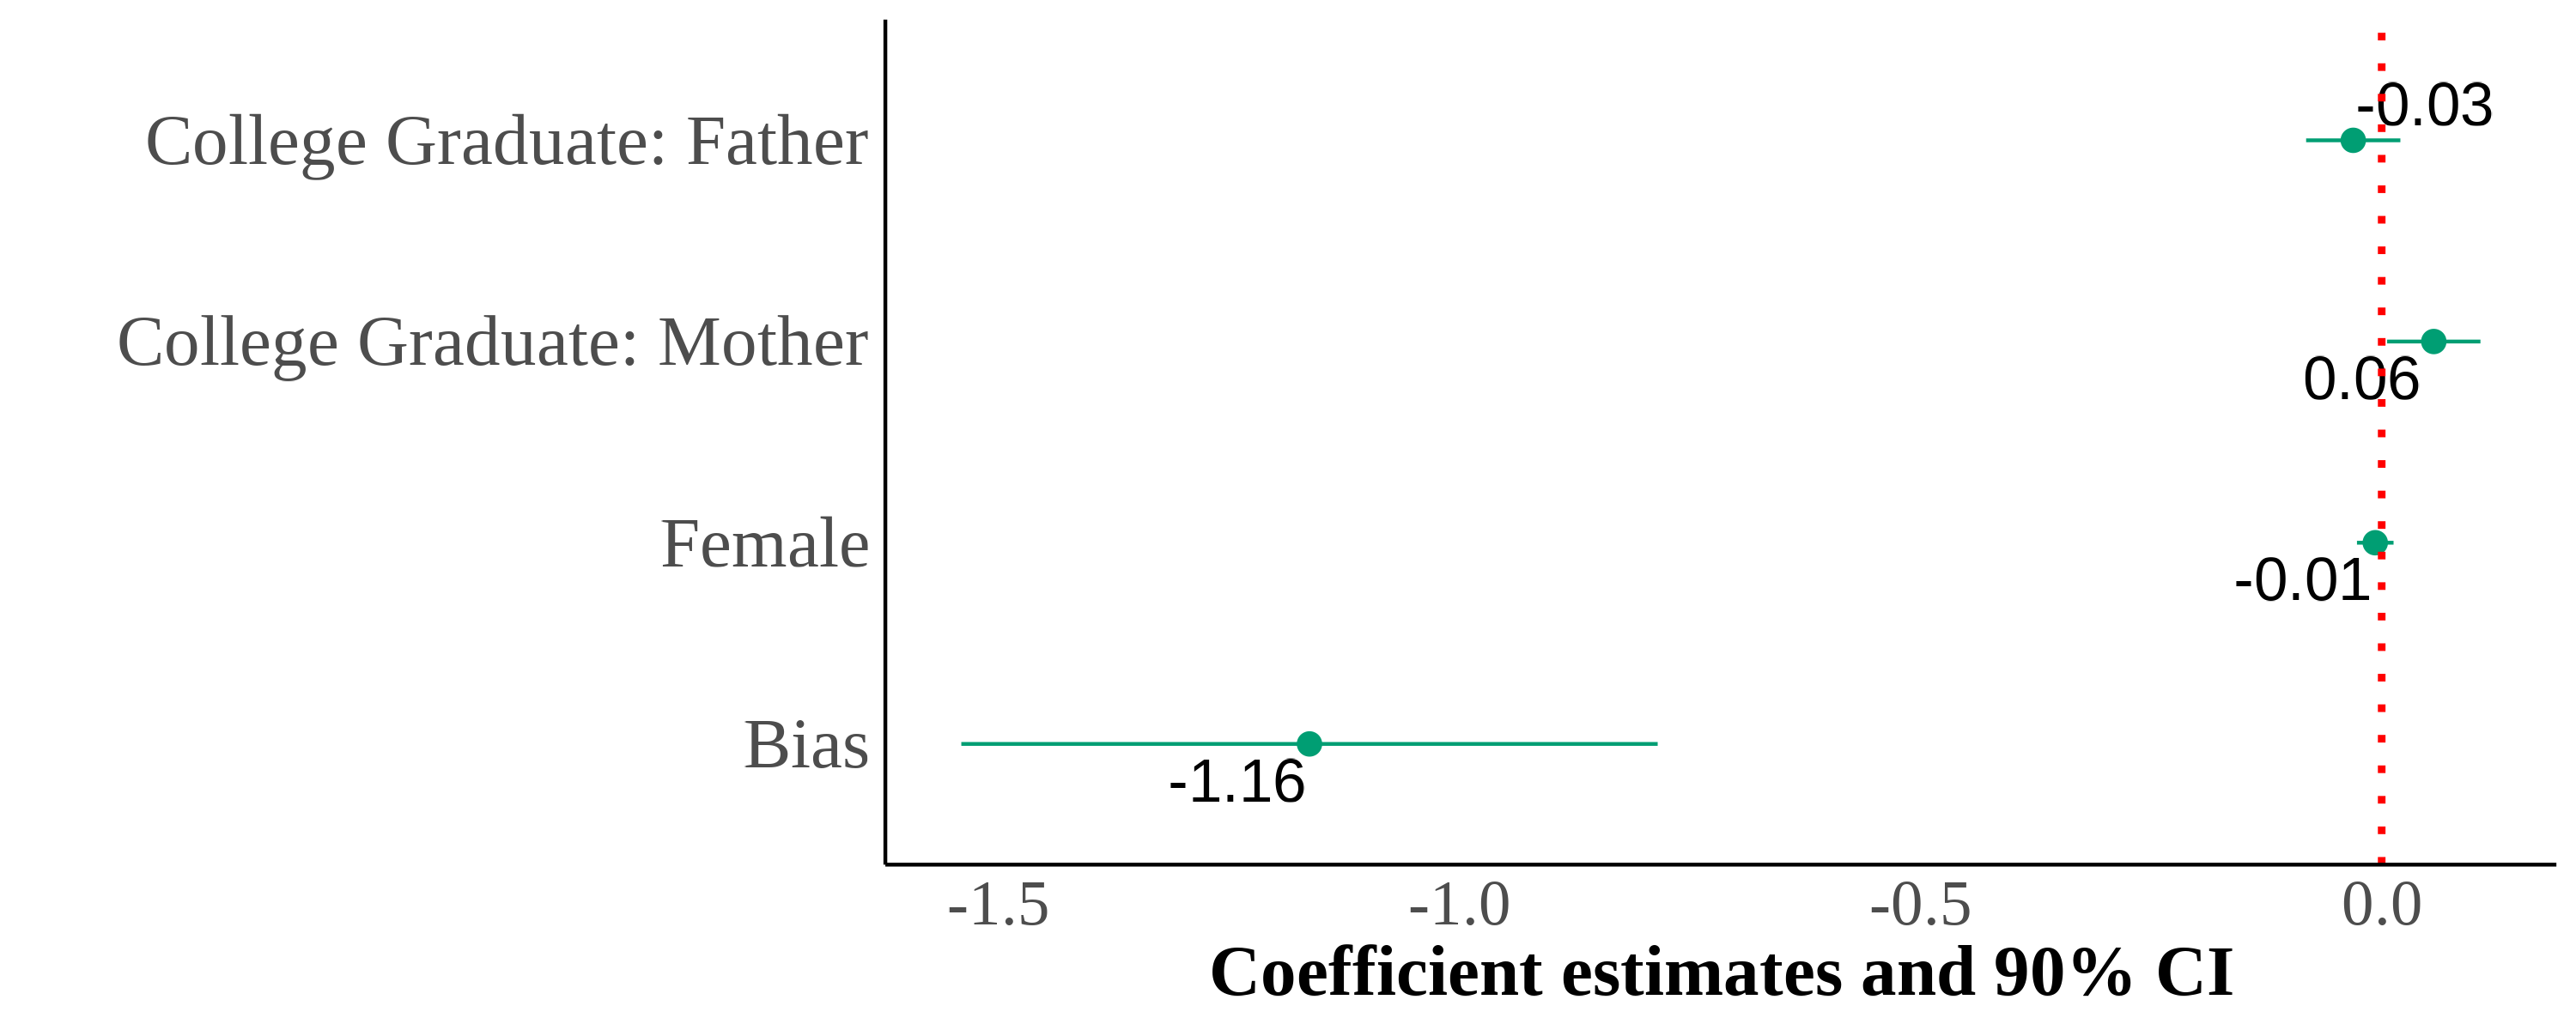
\includegraphics[width=.9\linewidth]{figure/by-parents-regs-hw.png}
\end{subfigure}
%Fourth Graph
\begin{subfigure}{.48\textwidth}
\caption{White Fathers-Hispanic Mothers}
\centering
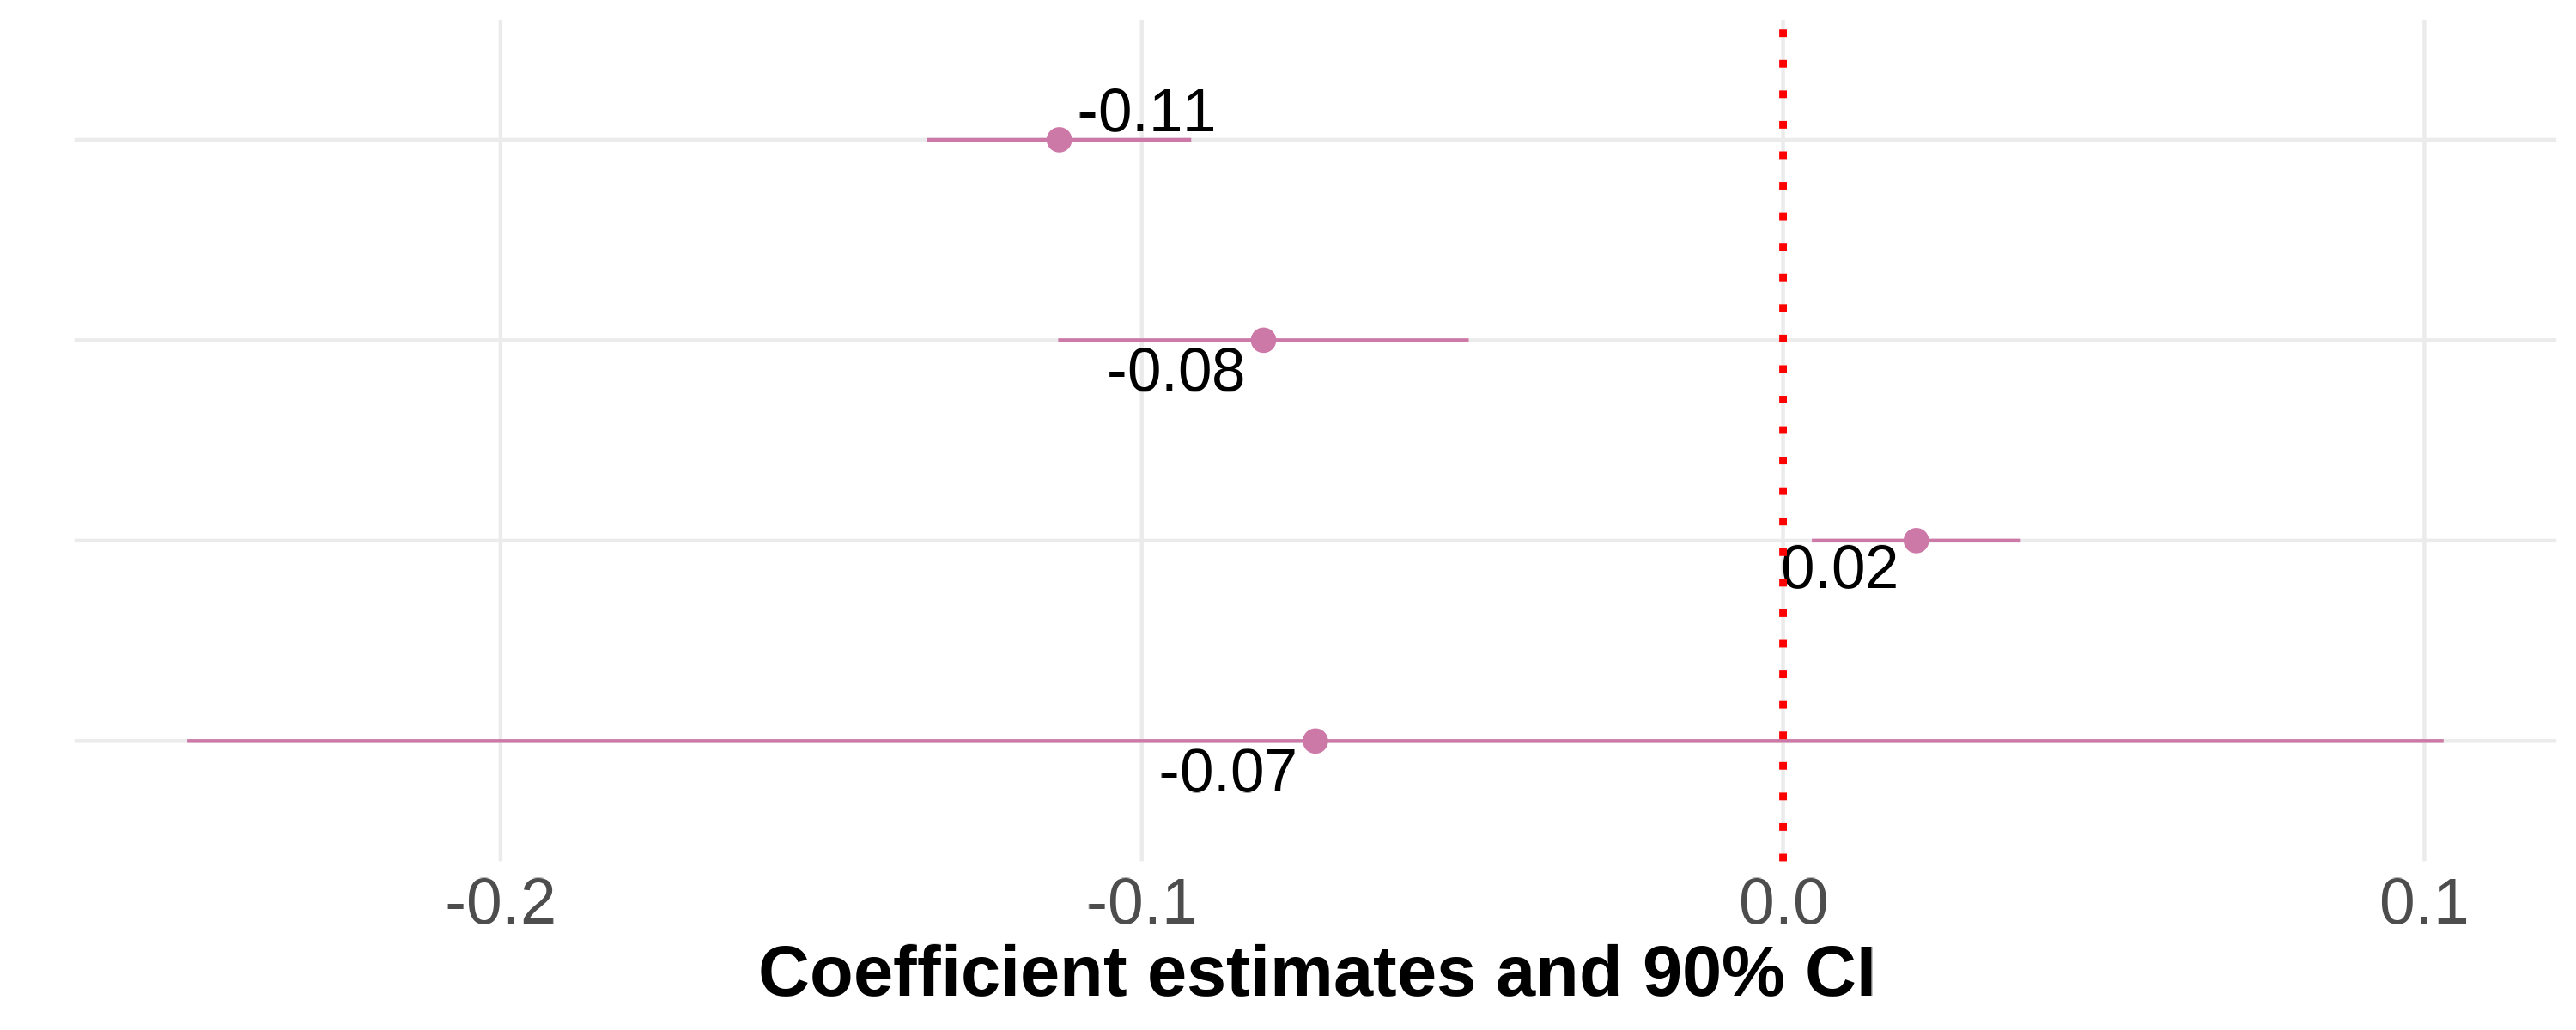
\includegraphics[width=.9\linewidth]{figure/by-parents-regs-wh.png}
\end{subfigure}
\flushleft\footnotesize{\note{I show four panels of estimating equation (\ref{eq:identity_reg_bias}). I include region $\times$ year fixed effects with controls for sex, quartic age, and parental education. The dependent variable is self-reported Hispanic identity and the independent variable is state-level bias. Each panel results from the same regression but on different samples divided by parental types. Standard errors are clustered on the state level. The samples include second-generation Hispanic children ages 17 and below who live in intact families. Native-born second-generation Hispanic immigrant children with at least one parent born in a Spanish-speaking country.}}
\end{figure}
\end{center}

\pagebreak
\newpage

\begin{table}[H]

\caption{Relationship Between Bias and Self-Reported Hispanic identity Among Third-Generation Hispanic Immigrants: By Grandparental Type \label{regtab-bygrandparents}}
\centering
\resizebox{\linewidth}{!}{
\begin{threeparttable}
\begin{tabular}[t]{lcccc}
\toprule
\multicolumn{1}{c}{ } & \multicolumn{4}{c}{Number of Hispanic Grandparents} \\
\cmidrule(l{3pt}r{3pt}){2-5}
  & \specialcell{(1) \\ One} & \specialcell{(2) \\ Two} & \specialcell{(3) \\ Three} & \specialcell{(4) \\ Four}\\
\midrule
Bias & -0.04 & 0.03 & 0.19 & -0.14*\\
 & (0.11) & (0.09) & (0.26) & (0.07)\\
Female & -0.01 & 0.00 & -0.01 & 0.00\\
 & (0.01) & (0.01) & (0.01) & (0.01)\\
College Graduate: Mother & -0.11*** & -0.07*** & 0.02 & -0.02\\
 & (0.03) & (0.02) & (0.02) & (0.01)\\
College Graduate: Father & -0.11*** & -0.08*** & 0.02 & -0.03*\\
 & (0.03) & (0.01) & (0.01) & (0.01)\\
\midrule
Observations & 55,051 & 74,100 & 12,194 & 57,646\\
Year $\times$ Region FE & X & X & X & X\\
\bottomrule
\multicolumn{5}{l}{\rule{0pt}{1em}* p $<$ 0.1, ** p $<$ 0.05, *** p $<$ 0.01}\\
\end{tabular}
\begin{tablenotes}
\small
\item[1] \footnotesize{Each column is an estimation of equation (\ref{eq:identity_reg_bias}) restricted to third-generation Hispanic immigrants by 
                      number of Hispanic grandparents with region × year fixed effects. 
                      I include controls for sex, quartic age, fraction of Hispanics in a state, and parental education.
                      Standard errors are clustered on the state level.}
\item[2] \footnotesize{The samples include third-generation Hispanic children ages 17 and below who live in intact families. 
                      Native-born third-generation Hispanic 
                      immigrant children with at least one grandparent born in a Spanish-speaking 
                      country.}
\item[3] \footnotesize{Data source is the 2004-2021 Current Population Survey.}
\end{tablenotes}
\end{threeparttable}}
\end{table}



\pagebreak
\newpage

\section{Robustness Checks and Discussions} % (fold)
\label{sec:results}

I will investigate the relationship between state-level bias and interethnic marriages. To this purpose, the regression specifications for the estimation will be as follows:

\begin{align}
Interethnic_{ist}^2 &= \beta_1^2 Bias_{st} + X_{ist}^2\pi + \gamma_{rt} 
            + \varepsilon_{ist}  \label{eq:inter-interethnic} 
\end{align}

Where $Interethnic_{ist}^2$ is an indicator variable that is equal to one if a couple is interethnic, i.e., a Hispanic husband-White wife or a White husband-Hispanic wife. $Bias_{st}$ is the average bias in state $s$ at time $t$, and $X_{ist}^2$ is a vector of partner-specific controls that would affect a marriage match that includes the wife's and husband's education, age, and years since immigrating to the United States. 

I present the results of estimating equation (\ref{eq:inter-interethnic}) in table (\ref{regtab-logit-02}). I find that a one standard deviation increase in bias increases the probability of having inter-ethnic parents by a 5 percentage point. Moreover, I break down the analysis by the ethnicity of the couples. A one standard deviation increase in state-level bias is associated a 6 percentage points increase in the chances of a Hispanic husband having a White wife. A one standard deviation increase in state-level bias is associated a 7 percentage points increase in the chances of a Hispanic wife having a White husband. The fact that bias and interethnic marriage are positively correlated could be a result of the fact that Hispanic immigrants in states with high bias might aim to decrease the likelihood that their children will display Hispanic ethnicity signals. For example, Hispanic women in high bias states might marry a non-Hispanic White husband, so their children will have a non-Hispanic last name.

I am also interested in investigating the relationship between state-level bias and migration. As the CPS does not report a person's birth state, I use the 2004-2021 Censuses to construct a sample of second-generation Hispanic immigrants \citep{floodsarahIntegratedPublicUse2021}. I construct a mover variable to indicate whether these second-generation Hispanic immigrants have moved from their birth state to another state. For this purpose, I use the following models to estimate the relationship between state-level bias and migration:

\begin{align}
BirthPlaceMigration_{ist}^2 &= \beta_1^2 Bias_{st} 
                   + X_{ist}^2\pi + \gamma_{rt} 
                   + \varepsilon_{ist} \label{eq:migration-3} \\
BirthPlaceMigration_{ilb}^2 &= \beta_1^2 Bias_{lb} 
                   + X_{ilb}^2\pi + \gamma_{lb} 
                   + \varepsilon_{ilb} \label{eq:migration-4}
\end{align}

Where $BirthPlaceMigration_{ist}^2$ is an indicator variable equal to one if person $i$ in state $s$ at the interview $t$ lives in a state that is different from his or her birth state and zero otherwise. $BirthPlaceMigration_{ilb}^2$ is an indicator variable that is equal to one if person $i$ in birthplace $l$ does not currently live in the same state he or she lived in at the year of birth $b$ and zero otherwise. The analysis, restricted to second-generation Hispanic immigrants with both parents born in a Spanish-speaking country, uses equations (\ref{eq:migration-3}) and (\ref{eq:migration-4}). 

Furthermore, I use two ways to define the bias variable to study the relationship between bias and the migration variables introduced above. In the first specification from equation (\ref{eq:migration-3}), I estimate the relationship between the average bias at the time of the interview $t$ in state $s$ and $BirthPlaceMigration_{ist}^2$. In the second specification from equation (\ref{eq:migration-4}), I estimate the relationship between the average bias in birth state $l$ at the year of birth $b$ and $BirthPlaceMigration_{ilb}^2$.

I also estimate whether those who self-identify as Hispanic tend to move from high-bias to low-bias states. The estimation equation for the relationship is: 

\begin{align}
Y_{ist} &= \beta_0 + \beta_1^2 Hispanic_{ist} +
                   X_{ist}^2\pi
                   + \varepsilon_{ist} \label{eq:migration-5}
\end{align}

Where $Y_{ist} \equiv Bias_{ist} -  Bias_{ilb}$, $Bias_{ist}$ is $i$'s state-level bias in state $s$ at the time of interview $t$, and  $Bias_{ilb}$ is $i$'s state-level bias in birth state $l$ at the birth year $b$. The analysis is restricted to second-generation Hispanic immigrants with both parents born in a Spanish-speaking country who migrated from the state they were born in $b$ to another state $s$. 

The results of estimating equations (\ref{eq:migration-3}), (\ref{eq:migration-4}), and (\ref{eq:migration-5}) are shown in table (\ref{regtab-mig-01}) in columns (1), (2), and (3) respectively. I find that among second-generation immigrants, there is no significant correlation between bias and migration decisions. Among second-generation Hispanic immigrant movers, those who self-report Hispanic identity live in states with 0.02 standard deviations more biased than the state where they were born. Even though this result shows that there is selection into more biased states among second-generation immigrants, it does not affect my main results showing a correlation between bias and self-reported Hispanic identity. Since those identifying as Hispanics are the movers, my assessments of the relationship between bias and self-reported Hispanic identity might underestimate the effect of bias.

\begin{table}[H]
\centering\centering
\caption{Relationship Between Bias and Interethnic Marriages \label{regtab-logit-02}}
\centering
\begin{threeparttable}
\begin{tabular}[t]{lccc}
\toprule
\multicolumn{2}{c}{ } & \multicolumn{1}{c}{Asian Men} & \multicolumn{1}{c}{Asian Women} \\
\cmidrule(l{3pt}r{3pt}){3-3} \cmidrule(l{3pt}r{3pt}){4-4}
  & \specialcell{(1) \\ Interethnic} & \specialcell{(2) \\ Interethnic} & \specialcell{(3) \\ Interethnic}\\
\midrule
Bias & $0.04$*** & $-0.01$ & $0.03$**\\
 & ($0.01$) & ($0.01$) & ($0.01$)\\
College Graduate: Wife & $0.04$*** & $0.04$*** & $0.05$***\\
 & ($0.00$) & ($0.01$) & \vphantom{1} ($0.00$)\\
College Graduate: Husband & $-0.01$* & $-0.01$ & $-0.02$***\\
 & ($0.00$) & ($0.01$) & ($0.00$)\\
\midrule
Observations & $69,800$ & $52,103$ & $60,214$\\
Year $\times$ Region FE & X & X & X\\
\bottomrule
\multicolumn{4}{l}{\rule{0pt}{1em}* p $<$ 0.1, ** p $<$ 0.05, *** p $<$ 0.01}\\
\end{tabular}
\begin{tablenotes}
\small
\item[1] \footnotesize{This is the result to estimating (\ref{eq:inter-interethnic}) as a
                      linear probability model.}
\item[2] \footnotesize{I include controls for partners' sex, age, education, 
                      and years since immigrating to the United States.
                      Standard errors are clustered on the household level.}
\item[3] \footnotesize{Data source is the 2004-2020 Current Population Survey Data.}
\end{tablenotes}
\end{threeparttable}
\end{table}


\begin{table}[H]

\caption{Relationship Between Bias and Migration \label{regtab-mig-01}}
\centering
\resizebox{\linewidth}{!}{
\begin{threeparttable}
\begin{tabular}[t]{lccc}
\toprule
  & \specialcell{(1) \\ Migrated from \\ Birth Place} & \specialcell{(2) \\ Migrated from \\ Birth Place} & \specialcell{(3) \\ $Bias_{ist} - Bias_{ilb}$}\\
\midrule
$Bias_{st}$ & 0.06 &  & \\
 & (0.12) &  & \\
$Bias_{lb}$ &  & -0.09 & \\
 &  & (0.26) & \\
Hispanic &  &  & 0.02***\\
 &  &  & (0.01)\\
Female & 0.00 & 0.00 & 0.00*\\
 & (0.00) & (0.00) & (0.00)\\
College Graduate: Mother & 0.03*** & 0.03*** & 0.00\\
 & (0.01) & (0.01) & \vphantom{1} (0.01)\\
College Graduate: Father & 0.02** & 0.02*** & -0.01\\
 & (0.01) & (0.01) & (0.01)\\
\midrule
Observations & 352,712 & 185,024 & 12,806\\
Mean & 0.09 & 0.09 & -0.02\\
Year $\times$ Region FE & X &  & \\
Birthyear $\times$ Birth Region FE &  & X & \\
\bottomrule
\multicolumn{4}{l}{\rule{0pt}{1em}* p $<$ 0.1, ** p $<$ 0.05, *** p $<$ 0.01}\\
\end{tabular}
\begin{tablenotes}
\small
\item[1] \footnotesize{Each column is an estimation of equations (\ref{eq:migration-3}) in column (1), 
                      (\ref{eq:migration-4}) in column (2), and
                      (\ref{eq:migration-5}) in column (3).}
\item[2] \footnotesize{Column (1) is a regression where the left hand side variable is 
                      a dummy variable that is equal to one if a person migrated from the state
                      were born in and the right hand side variable is bias the year of survey.
                      Column (2) is a regression where the left hand side variable is 
                      a dummy variable that is equal to one if a person migrated from the state
                      were born in and the right hand side variable is bias the year of birth in the state of birth.
                      Column (3) is a regression where the left hand side variable is 
                      the difference between state-level bias during the year of the survey in the current state the 
                      respondent is living in, and state-level bias during the year of birth in the state of birth 
                      and the right hand side variable is self-reported Hispanic identity. This regression captures
                      the selection of those that self-reported Hispanic identity into states with different levels of bias.
                      I include controls for sex, quartic age, parental education, fraction of Hispanics in a state, and region × year fixed effects.
                      Standard errors are clustered on the state level.}
\item[3] \footnotesize{The samples include children ages 17 and below who live in intact families. 
                      Native-born second-generation Hispanic immigrant children with both
                      parents born in a Spanish-speaking country. The sample in the column (3) regression is further restricted to only those that migrated from their birth state.}
\item[4] \footnotesize{Data source is the 2004-2021 Census Data.}
\end{tablenotes}
\end{threeparttable}}
\end{table}


The findings presented in this paper indicate a negative correlation between bias and the self-reported Hispanic identity of Hispanic immigrants. While my aim is not to establish a causal effect of bias on self-reported Hispanic identity, I intend to illustrate a correlation between bias and self-reported identity. This correlation suggests that depending on the levels of bias in a state, racial and ethnic gaps that rely on self-reported identity might either overestimate or underestimate the effect of discrimination.

There are a couple of concerns with this analysis. First, the self-reported identity in the Current Population Survey (CPS) is reported by a household respondent—parent or adult caregiver. Thus, the 'self-reported' ethnic identity might not reflect a child's true identity. I view the identity that a parent or a caregiver reports as an accurate representation of the child's identity since parents are essential in shaping their children's sense of self. Also, I compare states with a high and low bias for my analysis. The estimates will not be threatened as long as the likelihood of self-reporting does not differ between these states.

Moreover, \citet{duncanIntermarriageIntergenerationalTransmission2011} show that reported Hispanic identification does not vary with who is the household respondent. Additionally, I present the main effect of self-reported Hispanic identity by the household respondent in table (\ref{tab:hispbyproxy}) and the results to the estimation of equation (\ref{eq:identity_reg_bias}) by the proxy respondent in table (\ref{regtab-proxy-01}) across all generations. The main effect of the reported Hispanic identity of children is 94 percentage points when the mother is the proxy, 92 percentage points when the father is the proxy, and 96 percentage points when the child or another caregiver was the household respondent.\footnote{According to the Current Population Survey (CPS), a person can be the household respondent if they are at least 15 years old and have enough knowledge about the household. Thus, when the proxy is 'self,' the respondent is between the ages of 15 and 17.} The estimation of equation (\ref{eq:identity_reg_bias}) by the proxy respondent, table (\ref{regtab-proxy-01}), mostly yields a negative effect of bias on self-reported Hispanic identity for all types of proxy respondents.

\begin{table}[H]
\centering\centering
\caption{Main Effect of Proxy on Second-Generation's Asian Self-identification \label{tab:hispbyproxy}}
\centering
\fontsize{12}{14}\selectfont
\begin{tabular}[c]{>{}lllll}
\toprule
Parents Type & All & Asian-Asian & Asian-White & White-Asian\\
\midrule
\textbf{Proxy:} &  &  &  & \\
\hspace{1em}\textbf{Mother} & 0.72 & 0.97 & 0.37 & 0.3\\
\hspace{1em}\textbf{Father} & 0.72 & 0.97 & 0.39 & 0.29\\
\hspace{1em}\textbf{Self} & 0.87 & 0.97 & 0.23 & 0.31\\
\hspace{1em}\textbf{Others} & 0.88 & 0.96 & 0.6 & 0.54\\
\bottomrule
\end{tabular}
\end{table}


A second concern is that the IAT is voluntary and not representative of the population. While I do not claim that the IAT  as a proxy for bias will represent the population, \citet{egloffPredictiveValidityImplicit2002} show that they are hard to manipulate. Several studies have shown that IAT is correlated with economic outcomes \citep{chettyRaceEconomicOpportunity2020,gloverDiscriminationSelfFulfillingProphecy2017}, voting behavior \citep{friesePredictingVotingBehavior2007}, decision-making \citep{bertrandImplicitDiscrimination2005,carlanaImplicitStereotypesEvidence2019}, and health \citep{leitnerRacialBiasAssociated2016}. Another concern could be that the IAT test takers' characteristics change over time and, thus, are not the same. I address this concern by including non-parametric region $\times$ year fixed effects that would control for the systematic difference in the characteristics of test takers between regions. These changes will be controlled for as long as the differences in the characteristics between test takers do not vary across states within a region. 

Another concern could be reverse causality between having more Hispanic people in a state and implicit bias. It could be the case that the number of Hispanic people in a state affects the implicit bias on the residents of that state. For example, having more Hispanics in Florida could affect the implicit bias of the residents of Florida. To show that this is not the case, I provide figures (\ref{scatter-plot-1}) and (\ref{scatter-plot-4}) as evidence. Figure (\ref{scatter-plot-1}) plots the percent of self-reported Hispanics in a state at a specific year against the average implicit bias in the same state during that year. Figure (\ref{scatter-plot-4}) plots the percent of objectively second-generation Hispanic children of endogamous marriages in a state at a certain year against the average implicit bias in the same state during that year. I find no correlation between bias and the number of Hispanics in a state, thus, making the case of reverse causality unlikely. 

Finally, the estimator of the relationship between bias (prejudice) and self-reported Hispanic identity could be biased if those that do not self-report Hispanic identity migrate to more prejudiced states. I have shown above that this is not the case (table \ref{regtab-mig-01}). I find no evidence of a relationship between migration decisions and bias. Additionally, I find that those reporting Hispanic identity moved out of birthplaces with less bias and lived in more biased states at the time of the survey. Thus, my results might underestimate the relationship between bias and self-reported Hispanic identity.

\section{Conclusion}\label{sec:conc}

As the United States becomes more multi-racial and multi-ethnic, self-reported identity will significantly affect on representation, distributive politics, and government transfers. The determinants of endogenous identity are particularly important to researchers interested in the role of discrimination on earnings gaps. In this paper, I show how individual characteristics and social attitudes toward racial and ethnic minorities affect the self-reported Hispanic identity of individuals with Hispanic ancestry in the United States. I find that people of Hispanic ancestry are less likely to identify as Hispanic in states with more significant bias. The relationship between self-reported Hispanic identity and bias is more prominent among first- and second-generation immigrants, where a one standard deviation increase in bias correlated with a 7 and 13 percentage points decrease in self-reported Hispanic identity. 

Additionally, state-level bias has a more substantial effect among second-generation immigrant children with Hispanic fathers and Hispanic mothers. A one standard deviation increase in bias correlates with a 15 percentage points decrease in self-reported Hispanic identity among second-generation Hispanic immigrant children of objectively Hispanic parents. I also find that bias positively correlates with interethnic marriage and not with migration decisions.

The results are important because of the consequences on the correct counting of Hispanics and minorities, and  assimilation and mobility. They could indicate that bias could significantly affect how economists estimate the earnings gap. Most research concerning race and ethnicity relies on self-reported race and ethnic identity measures. Since state-level bias is negatively correlated with self-reported Hispanic identity, the characteristics of those who do not self-report Hispanic identity could have important consequences. For example, if the people whose identities are most likely affected by bias are the most educated. In this case, the racial and ethnic gaps will be overestimated in the most biased states. Furthermore, identity decisions are likely to affect people's choices, investments, and well-being profoundly. 

Moreover, this study could encourage further research into the relationship between bias and self-reported identities for other groups. The analysis of the effect of bias on self-reported identity could be applied to other groups. For example, we could estimate the effect of bias on the identities of sexual minorities and other ethnic and racial minorities such as Asian American, Black, Native American, and Arab American populations in the United States. Researchers could also explore the differences in outcomes between the ethnic and racial minorities who self-report to those that do not by using restricted administrative data. 

\newpage
\pagebreak

\begin{appendices}

\section{Tables}\label{appendix:tabs}

\begin{table}[!h]
\centering\centering
\caption{Relationship Between Bias and Self-Reported Asian Identity: By Proxy Respondent\label{regtab-proxy-01}}
\centering
\resizebox{\ifdim\width>\linewidth\linewidth\else\width\fi}{!}{
\begin{threeparttable}
\begin{tabular}[t]{lcccccc}
\toprule
\multicolumn{1}{c}{ } & \multicolumn{6}{c}{Proxy Respondent} \\
\cmidrule(l{3pt}r{3pt}){2-7}
\multicolumn{1}{c}{ } & \multicolumn{1}{c}{White Mother} & \multicolumn{1}{c}{Asian Mother} & \multicolumn{1}{c}{White Father} & \multicolumn{1}{c}{Asian Father} & \multicolumn{1}{c}{Self} & \multicolumn{1}{c}{Other} \\
\cmidrule(l{3pt}r{3pt}){2-2} \cmidrule(l{3pt}r{3pt}){3-3} \cmidrule(l{3pt}r{3pt}){4-4} \cmidrule(l{3pt}r{3pt}){5-5} \cmidrule(l{3pt}r{3pt}){6-6} \cmidrule(l{3pt}r{3pt}){7-7}
  & \specialcell{(1) \\ $A_{ist}$} & \specialcell{(2) \\ $A_{ist}$} & \specialcell{(3) \\ $A_{ist}$} & \specialcell{(4) \\ $A_{ist}$} & \specialcell{(5) \\ $A_{ist}$} & \specialcell{(6) \\ $A_{ist}$}\\
\midrule
Prejudice Measure & 0.04 & -0.06 & -0.09 & 0.03 & 0.02 & 0.07\\
 & (0.07) & (0.05) & (0.06) & (0.03) & (0.07) & (0.06)\\
Female & -0.02 & 0.01 & -0.01 & 0.00 & -0.07* & 0.00\\
 & (0.02) & (0.01) & (0.02) & (0.01) & (0.04) & (0.01)\\
College Graduate: Mother & 0.01 & -0.04** & -0.02 & 0.00 & -0.05 & -0.07***\\
 & (0.03) & (0.01) & (0.02) & (0.01) & (0.05) & (0.01)\\
College Graduate: Father & 0.00 & 0.00 & 0.02 & 0.01 & -0.02 & -0.02\\
 & (0.03) & (0.02) & (0.02) & (0.01) & (0.06) & (0.01)\\
Second Gen & -0.06 & -0.10*** & 0.17 & -0.18*** & -1.02*** & -0.44***\\
 & (0.04) & (0.04) & (0.18) & (0.05) & (0.05) & (0.05)\\
\midrule
Observations & 4,330 & 28,374 & 8,686 & 28,506 & 738 & 5,823\\
Year $\times$ Region FE & X & X & X & X & X & X\\
\bottomrule
\multicolumn{7}{l}{\rule{0pt}{1em}* p $<$ 0.1, ** p $<$ 0.05, *** p $<$ 0.01}\\
\end{tabular}
\begin{tablenotes}
\small
\item[1] \footnotesize{Each column is an estimation of a heterogeneous effect of regression (\ref{eq:identity_reg_bias}) by 
                      the proxy household respondent with region × year fixed effects. 
                      I include controls for sex, quartic age, fraction of Asians in a state, parental education.
                      Standard errors are clustered on the state level.}
\item[2] \footnotesize{The samples include children ages 17 and below who live in intact families. 
                      First-generation Asian immigrant children that were born in a 
                      Spanish-speaking county. Native-born second-generation Asian 
                      immigrant children with at least one parent born in an Asian 
                      country. Finally, native-born third-generation Asian immigrant children 
                      with native-born parents and at least one grandparent born in a Spanish 
                      speaking country.}
\item[3] \footnotesize{Data source is the 2004-2021 Current Population Survey.}
\end{tablenotes}
\end{threeparttable}}
\end{table}


\pagebreak
\newpage

% \begin{table}[!h]

\caption{Relationship Between Bias and Self-Reported Hispanic Identity \label{regtab-01}}
\centering
\resizebox{\linewidth}{!}{
\begin{threeparttable}
\begin{tabular}[t]{lccccc}
\toprule
  & \specialcell{(1) \\ $H_i$} & \specialcell{(2) \\ $H_i$} & \specialcell{(3) \\ $H_i$} & \specialcell{(4) \\ $H_i$} & \specialcell{(5) \\ $H_i$}\\
\midrule
Bias & -0.04 & 0.00 & -0.03*** & 0.03 & -0.10**\\
 & (0.03) & (0.05) & (0.01) & (0.03) & (0.04)\\
Female & 0.00 & 0.00 & 0.00 & 0.00 & 0.00\\
 & (0.00) & (0.00) & (0.00) & (0.00) & (0.00)\\
College Graduate: Mother & -0.05*** & -0.06*** & -0.05*** & -0.05*** & -0.05***\\
 & (0.01) & (0.01) & (0.01) & (0.01) & (0.01)\\
College Graduate: Father & -0.07*** & -0.07*** & -0.06*** & -0.06*** & -0.06***\\
 & (0.00) & (0.00) & (0.01) & (0.01) & (0.01)\\
First Gen & -1.18*** & 0.13*** & 0.36*** & 0.04*** & 0.26***\\
 & (0.02) & (0.01) & (0.03) & (0.01) & (0.03)\\
Second Gen & -1.20*** & 0.11*** & 0.34*** & 0.02*** & 0.24***\\
 & (0.02) & (0.01) & (0.02) & (0.01) & (0.03)\\
\midrule
Observations & 844,481 & 844,481 & 844,481 & 844,481 & 844,481\\
Mean & 0.91 & 0.91 & 0.91 & 0.91 & 0.91\\
State FE &  &  & X & X & \\
Year FE &  & X &  & X & \\
Year $\times$ Region FE &  &  &  &  & X\\
\bottomrule
\multicolumn{6}{l}{\rule{0pt}{1em}* p $<$ 0.1, ** p $<$ 0.05, *** p $<$ 0.01}\\
\end{tabular}
\begin{tablenotes}
\small
\item[1] \footnotesize{Each column is an estimation of a regression the following regression 
                      (\ref{eq:identity_reg_bias}) with different set of
                      fixed effects. I include controls for sex, quartic age, parental education, fraction of Hispanics in a state, and generational, parents' and grandparents' type dummy variables.
                      Standard errors are clustered on the state level.}
\item[2] \footnotesize{The samples include children ages 17 and below who live in intact families. 
                      First-generation Hispanic immigrant children that were born in a 
                      Spanish-speaking county. Native-born second-generation Hispanic 
                      immigrant children with at least one parent born in a Spanish-speaking 
                      country. Finally, native-born third-generation Hispanic immigrant children 
                      with native-born parents and at least one grandparent born in a Spanish 
                      speaking country.}
\item[3] \footnotesize{Data source is the 2004-2021 Current Population Survey.}
\end{tablenotes}
\end{threeparttable}}
\end{table}



% \pagebreak
% \newpage

% \begin{table}[!h]
\centering\centering
\caption{Relationship Between Bias and Self-Reported Asian Identity: By Generation \label{regtab-bygen-01}}
\centering
\resizebox{\ifdim\width>\linewidth\linewidth\else\width\fi}{!}{
\begin{threeparttable}
\begin{tabular}[t]{lcccc}
\toprule
  & \specialcell{(1) \\ All Gens \\ $H_{ist}$} & \specialcell{(2) \\  First Gen \\ $H^1_{ist}$} & \specialcell{(3) \\  Second Gen \\ $H^2_{ist}$} & \specialcell{(4) \\  Third Gen \\ $H^3_{ist}$}\\
\midrule
Bias & -0.06** & -0.05 & -0.08** & -0.08**\\
 & (0.02) & (0.04) & (0.03) & (0.03)\\
Female & 0.00 & -0.01 & 0.00 & -0.01\\
 & (0.00) & (0.01) & (0.00) & (0.01)\\
College Graduate: Mother & 0.00 & -0.01 & 0.01 & 0.03\\
 & (0.01) & (0.01) & (0.01) & \vphantom{1} (0.02)\\
College Graduate: Father & 0.00 & 0.02** & 0.00 & -0.01\\
 & (0.01) & (0.01) & (0.01) & (0.02)\\
\midrule
Observations & 129,078 & 15,499 & 80,137 & 33,442\\
Mean & 0.65 & 0.44 & 0.22 & 0.66\\
Year $\times$ Region FE & X & X & X & X\\
\bottomrule
\multicolumn{5}{l}{\rule{0pt}{1em}* p $<$ 0.1, ** p $<$ 0.05, *** p $<$ 0.01}\\
\end{tabular}
\begin{tablenotes}
\small
\item[1] \footnotesize{Each column is an estimation of a heterogeneous effect of regression (\ref{eq:identity_reg_bias}) by 
                      generation with region × year fixed effects. 
                      I include controls for sex, quartic age, fraction of Asians in a state, and parental education.
                      I also added parents' (HH, HW, and WH) and grandparents' (HHHH, HHHW, HHWH, etc.) type dummy variables to the regression
                      on second and third generation immigrants, where H is objectively Asian (born in a Asian country) and W is objectively White (native-born). 
                      Standard errors are clustered on the state level.}
\item[2] \footnotesize{The samples include children ages 17 and below who live in intact families. 
                      First-generation Asian immigrant children that were born in a 
                      Asian country. Native-born second-generation Asian 
                      immigrant children with at least one parent born in a Asian 
                      country. Finally, native-born third-generation Asian immigrant children 
                      with native-born parents and at least one grandparent born in a Asian country.}
\item[3] \footnotesize{Data source is the 2004-2021 Current Population Survey.}
\end{tablenotes}
\end{threeparttable}}
\end{table}


% \begin{table}[H]

\caption{Relationship Between Bias and Self-Reported Hispanic identity Among Second-Generation Hispanic Immigrants: By Parental Type \label{regtab-byparent-01}}
\centering
\resizebox{\linewidth}{!}{
\begin{threeparttable}
\begin{tabular}[t]{lcccc}
\toprule
\multicolumn{1}{c}{Parents Type} & \multicolumn{1}{c}{All} & \multicolumn{1}{c}{\makecell[c]{Both Parents \\ from Spanish \\ Speaking Country \\ (HH)}} & \multicolumn{1}{c}{\makecell[c]{Father \\ from Spanish \\ Speaking Country \\ (HW)}} & \multicolumn{1}{c}{\makecell[c]{Mother  \\ from Spanish \\ Speaking Country \\ (WH)}} \\
\cmidrule(l{3pt}r{3pt}){1-1} \cmidrule(l{3pt}r{3pt}){2-2} \cmidrule(l{3pt}r{3pt}){3-3} \cmidrule(l{3pt}r{3pt}){4-4} \cmidrule(l{3pt}r{3pt}){5-5}
  & \specialcell{(1) \\ $H^2_{ist}$} & \specialcell{(2) \\ $H^2_{ist}$} & \specialcell{(3) \\ $H^2_{ist}$} & \specialcell{(4) \\ $H^2_{ist}$}\\
\midrule
Bias & -0.13** & -0.15** & -0.01 & -0.07\\
 & (0.05) & (0.06) & (0.07) & (0.10)\\
Female & 0.00 & 0.00 & -0.01 & 0.02**\\
 & (0.00) & (0.00) & (0.01) & (0.01)\\
College Graduate: Mother & -0.06*** & -0.04*** & -0.07*** & -0.08***\\
 & (0.01) & (0.01) & (0.01) & (0.02)\\
College Graduate: Father & -0.08*** & -0.04*** & -0.10*** & -0.11***\\
 & (0.01) & (0.01) & (0.02) & (0.01)\\
\midrule
Observations & 560,100 & 405,116 & 88,421 & 66,563\\
Year $\times$ Region FE & X & X & X & X\\
Mean & 0.94 & 0.96 & 0.9 & 0.83\\
\bottomrule
\multicolumn{5}{l}{\rule{0pt}{1em}* p $<$ 0.1, ** p $<$ 0.05, *** p $<$ 0.01}\\
\end{tabular}
\begin{tablenotes}
\small
\item[1] \footnotesize{Each column is an estimation of a heterogeneous effect of regression (\ref{eq:identity_reg_bias}) by 
                      type of parents with region × year fixed effects. 
                      I include controls for sex, quartic age, fraction of Hispanics in a state, and parental education.
                      Standard errors are clustered on the state level.}
\item[2] \footnotesize{The samples include second-generation Hispanic children ages 17 and below who live in intact families. 
                      Native-born second-generation Hispanic 
                      immigrant children with at least one parent born in a Spanish-speaking 
                      country.}
\item[3] \footnotesize{Column (1) includes the results to regression (\ref{eq:identity_reg_bias}) on all second-generation immigrants, 
                                        column (2) includes the results to regression (\ref{eq:identity_reg_bias}) on second-generation immigrants that who has a father and mother that were born in a Spanish-speaking country (HH),
                                        column (3) includes the results to regression (\ref{eq:identity_reg_bias}) on second-generation immigrants that who has a father that was born in a Spanish-speaking country and a native-born mother (HW), and
                                        column (4) includes the results to regression (\ref{eq:identity_reg_bias}) on second-generation immigrants that who has a native-born father and a mother that was born in a Spanish-speaking country (WH).}
\item[4] \footnotesize{Data source is the 2004-2021 Current Population Survey.}
\end{tablenotes}
\end{threeparttable}}
\end{table}


% \pagebreak
% \newpage


\section{Figures}\label{appendix:figs}

% \begin{center}
% \begin{figure}[H]
% \caption{Proportion of Hispanics in the United States from 1995 to 2019}
% \label{fig:hisp}
% 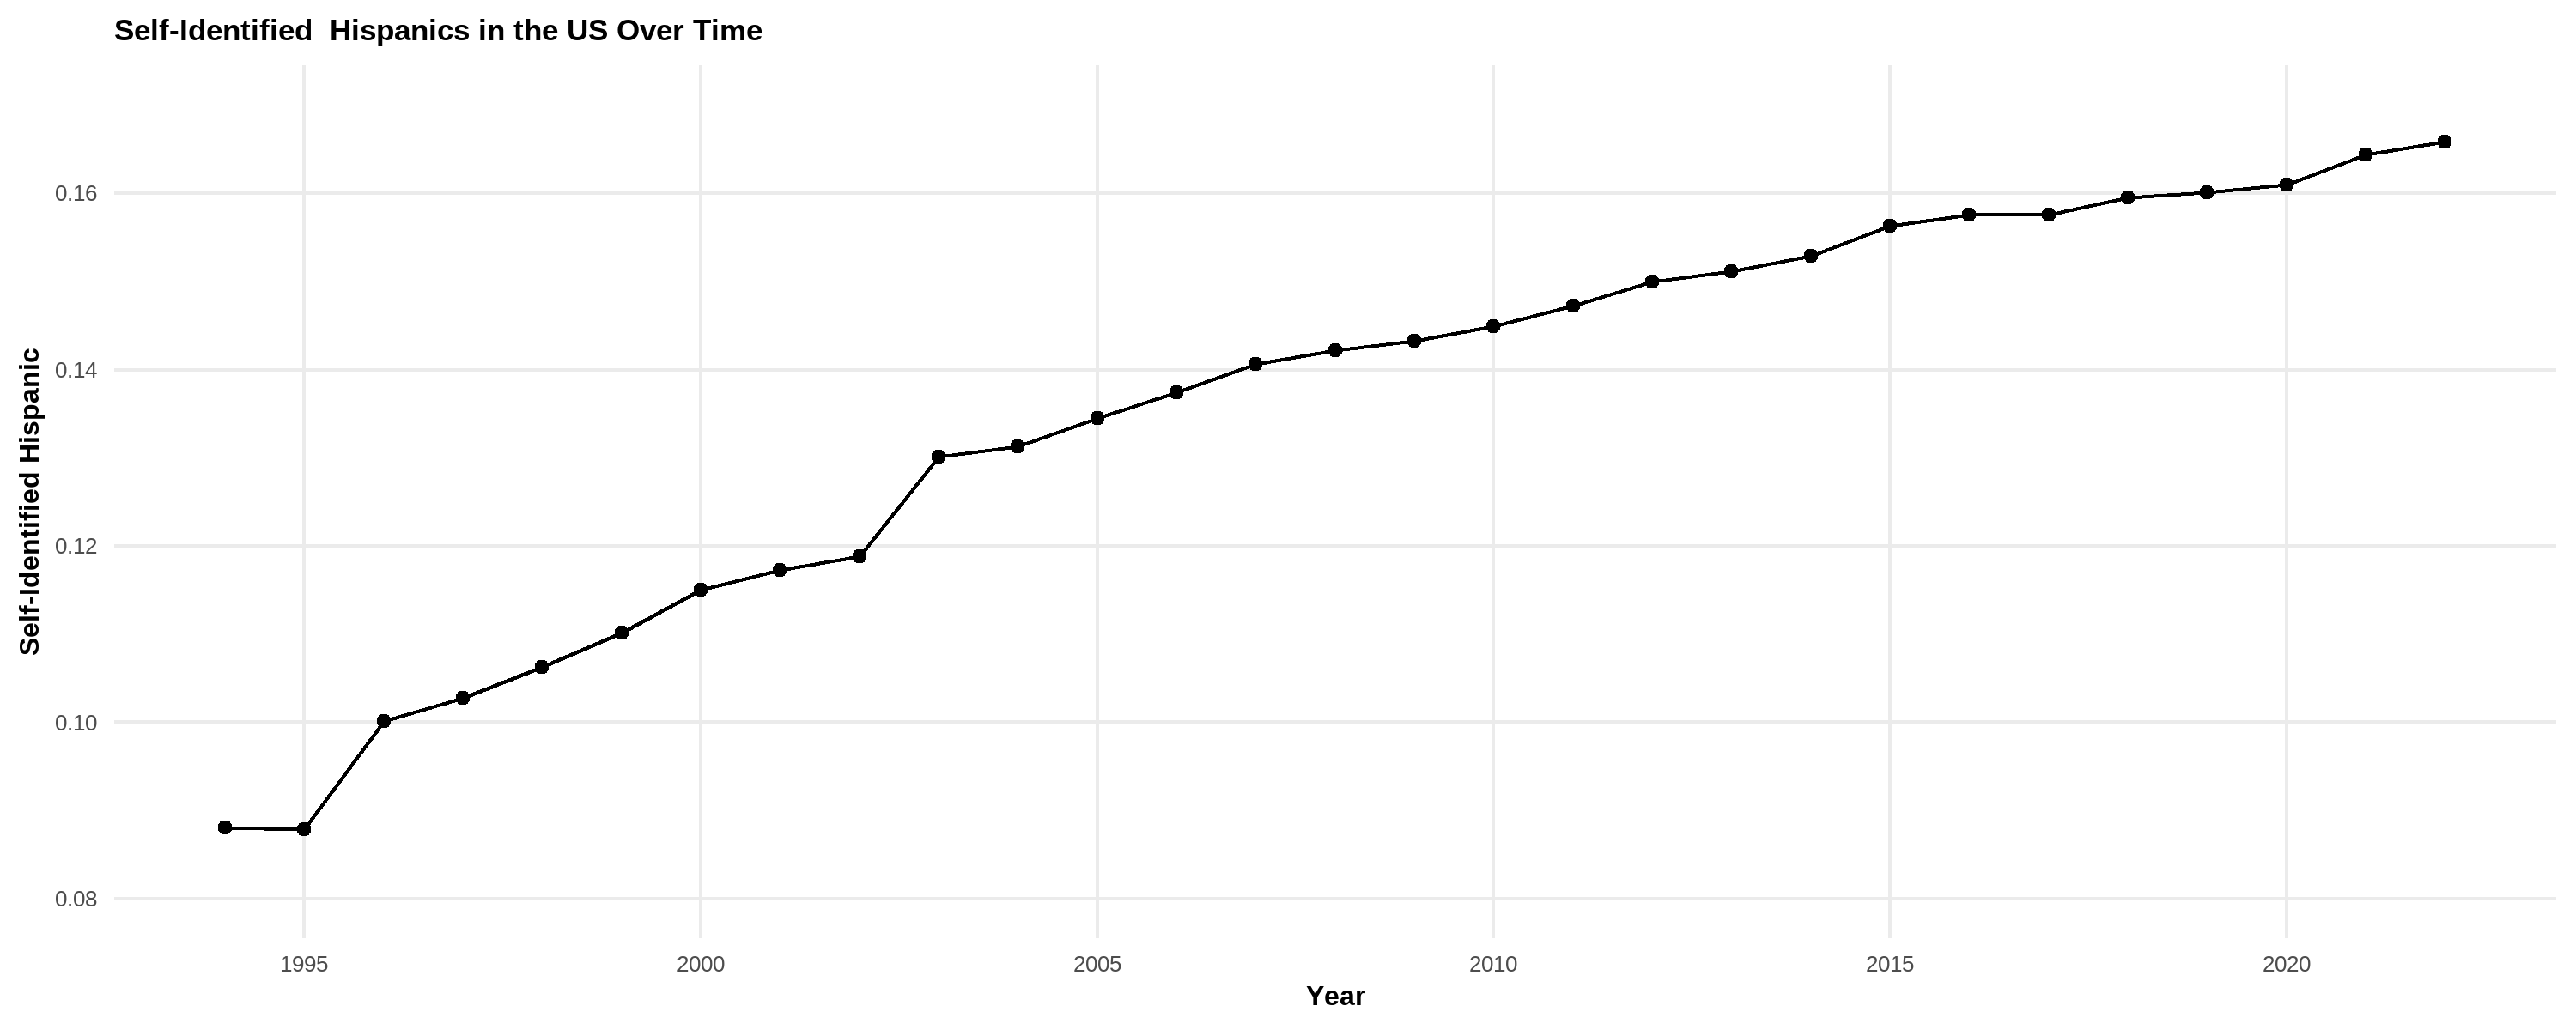
\includegraphics[width=\textwidth,scale=0.8]{figure/Hispanics_all.png} 
% \end{figure}
% \flushleft\footnotesize{\note{Data source is the Current Population Survey (CPS) from 1994 to 2021. The number of Hispanics in the United States doubled between 1994 and 2021. The number of Hispanics increased from 9\% in 1994 to 17\% in 2021.}}
% \end{center}

% \pagebreak
% \newpage


\begin{figure}[!htb]
\centering
\caption{Scatter Plot of Proportion Subjectively Hispanic on Bias}
\label{scatter-plot-1}
\begin{subfigure}{.9\textwidth}
\caption{Year < 2015}
\centering
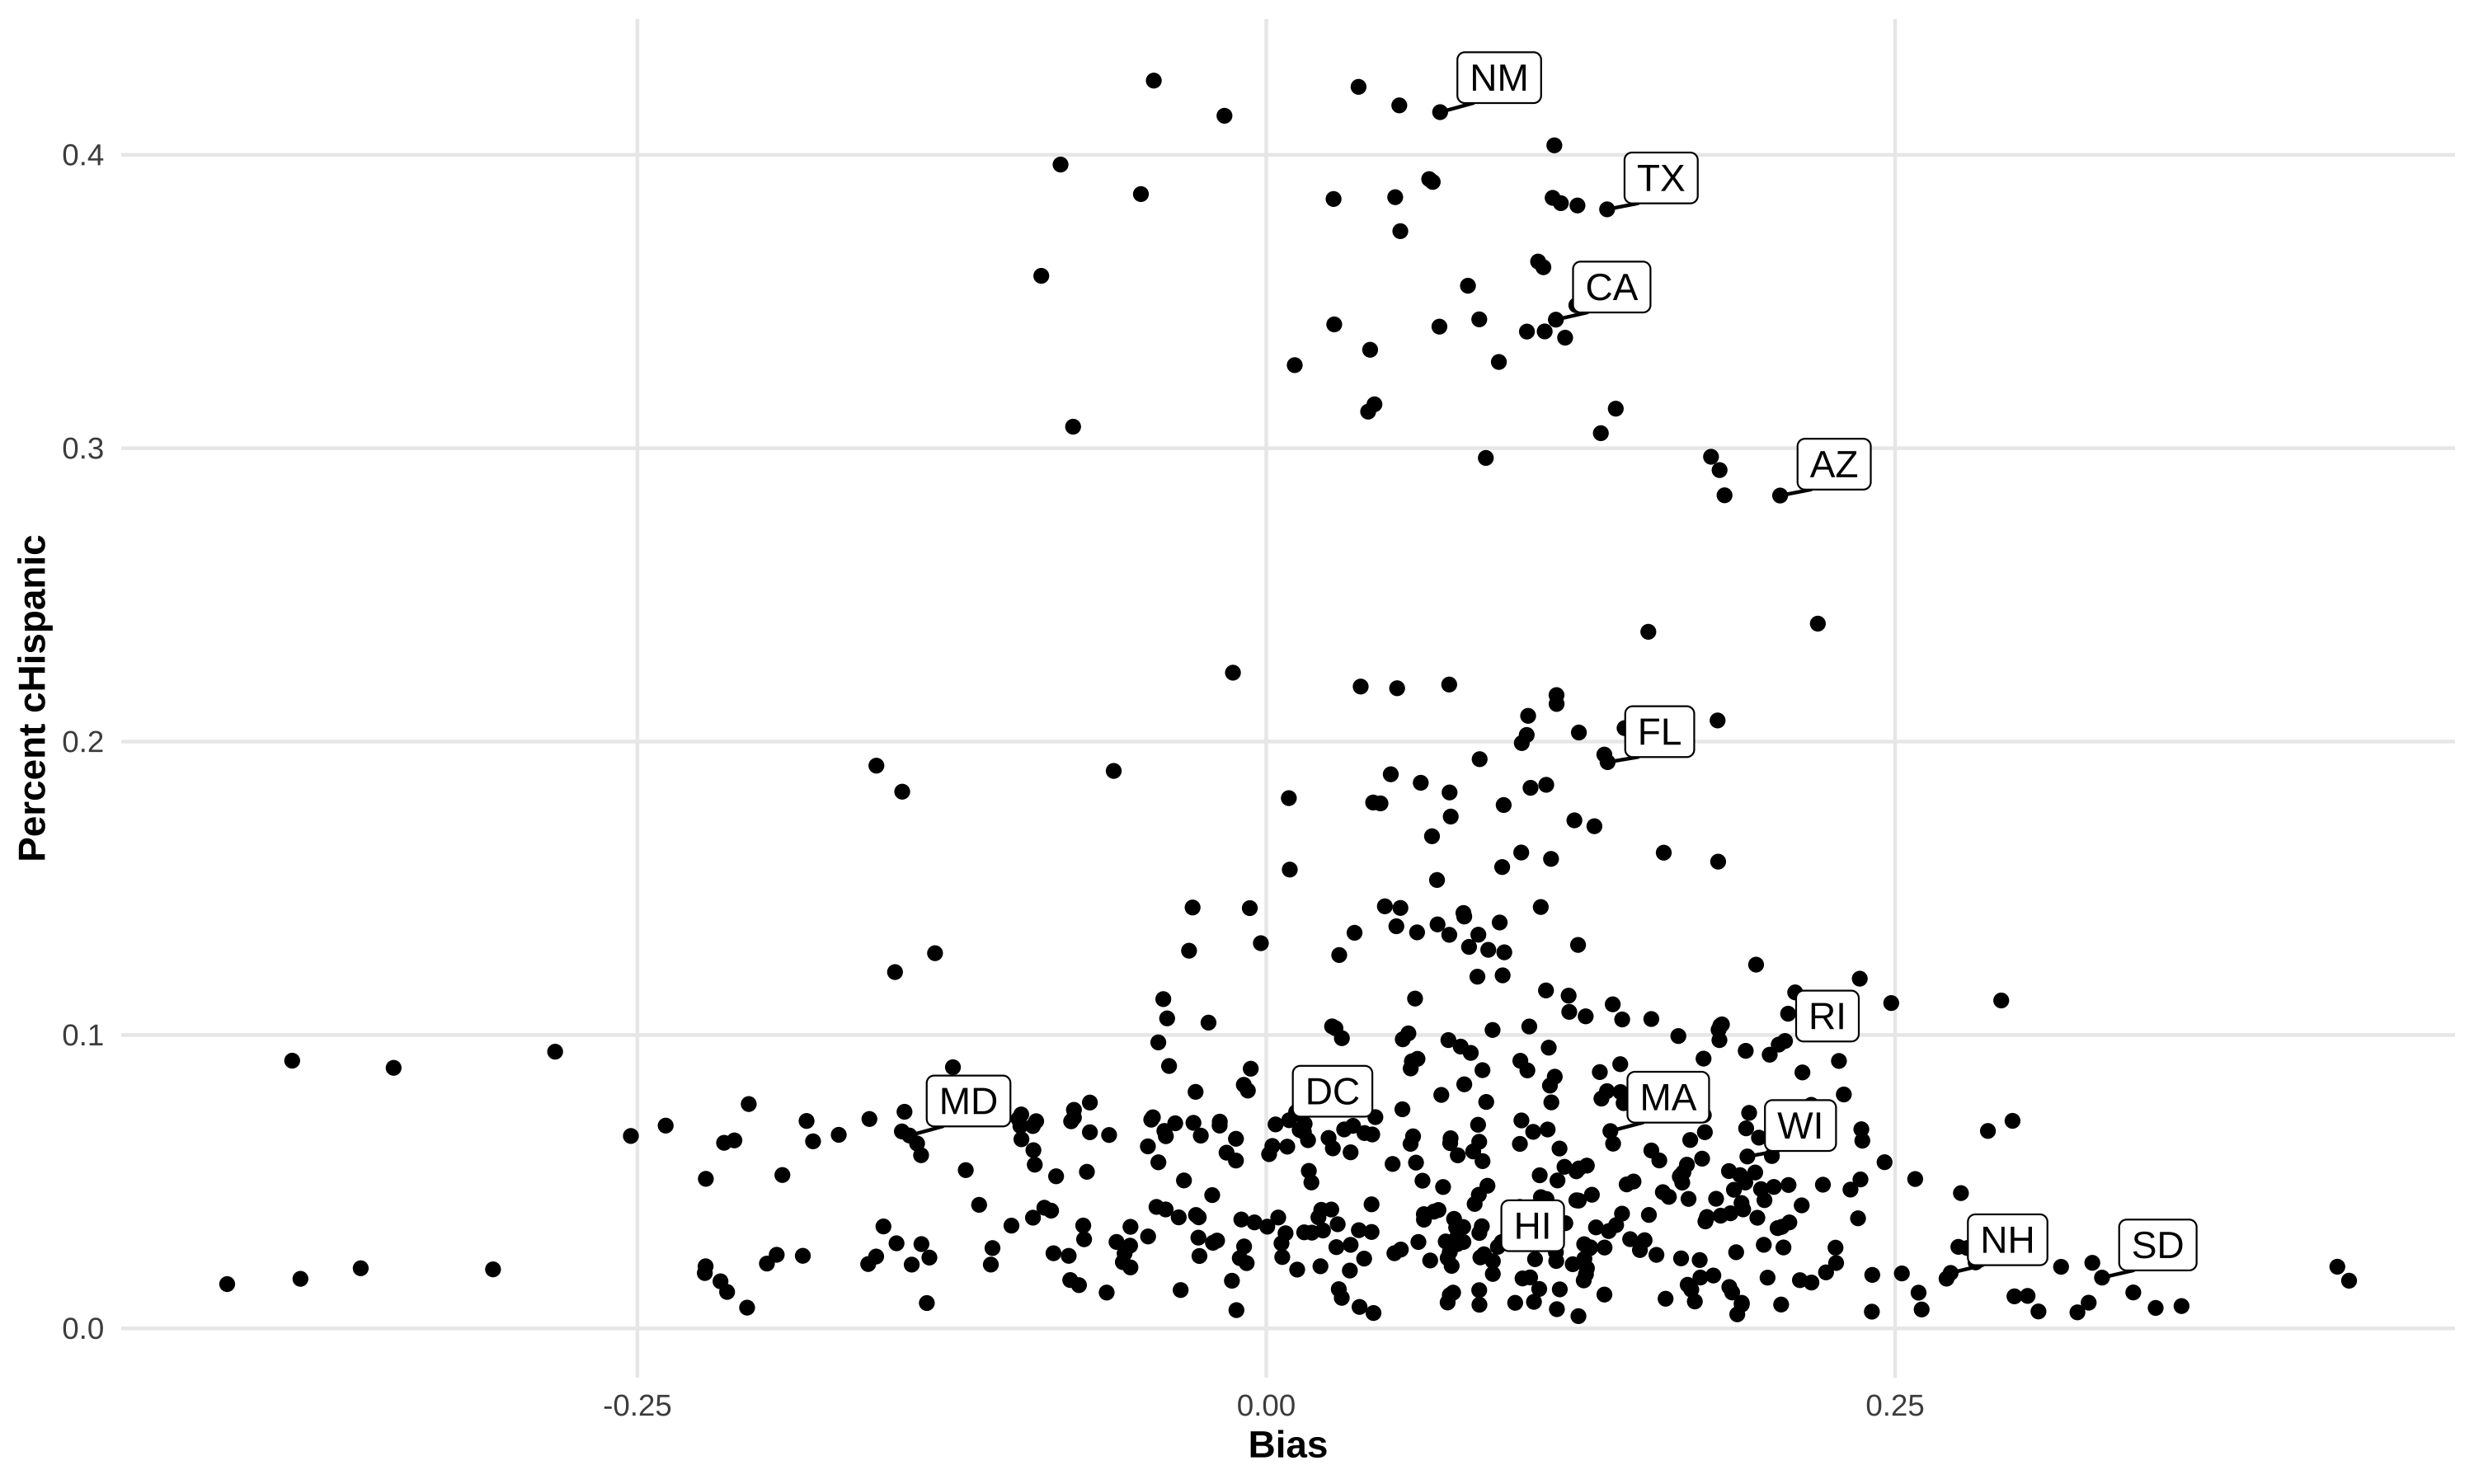
\includegraphics[width=.9\linewidth]{figure/scatter-plot-bias-hispanic-less2015.png}
\end{subfigure}
\centering
%Second graph
\begin{subfigure}{.9\textwidth}
\caption{Year $\geq$ 2015}
\centering
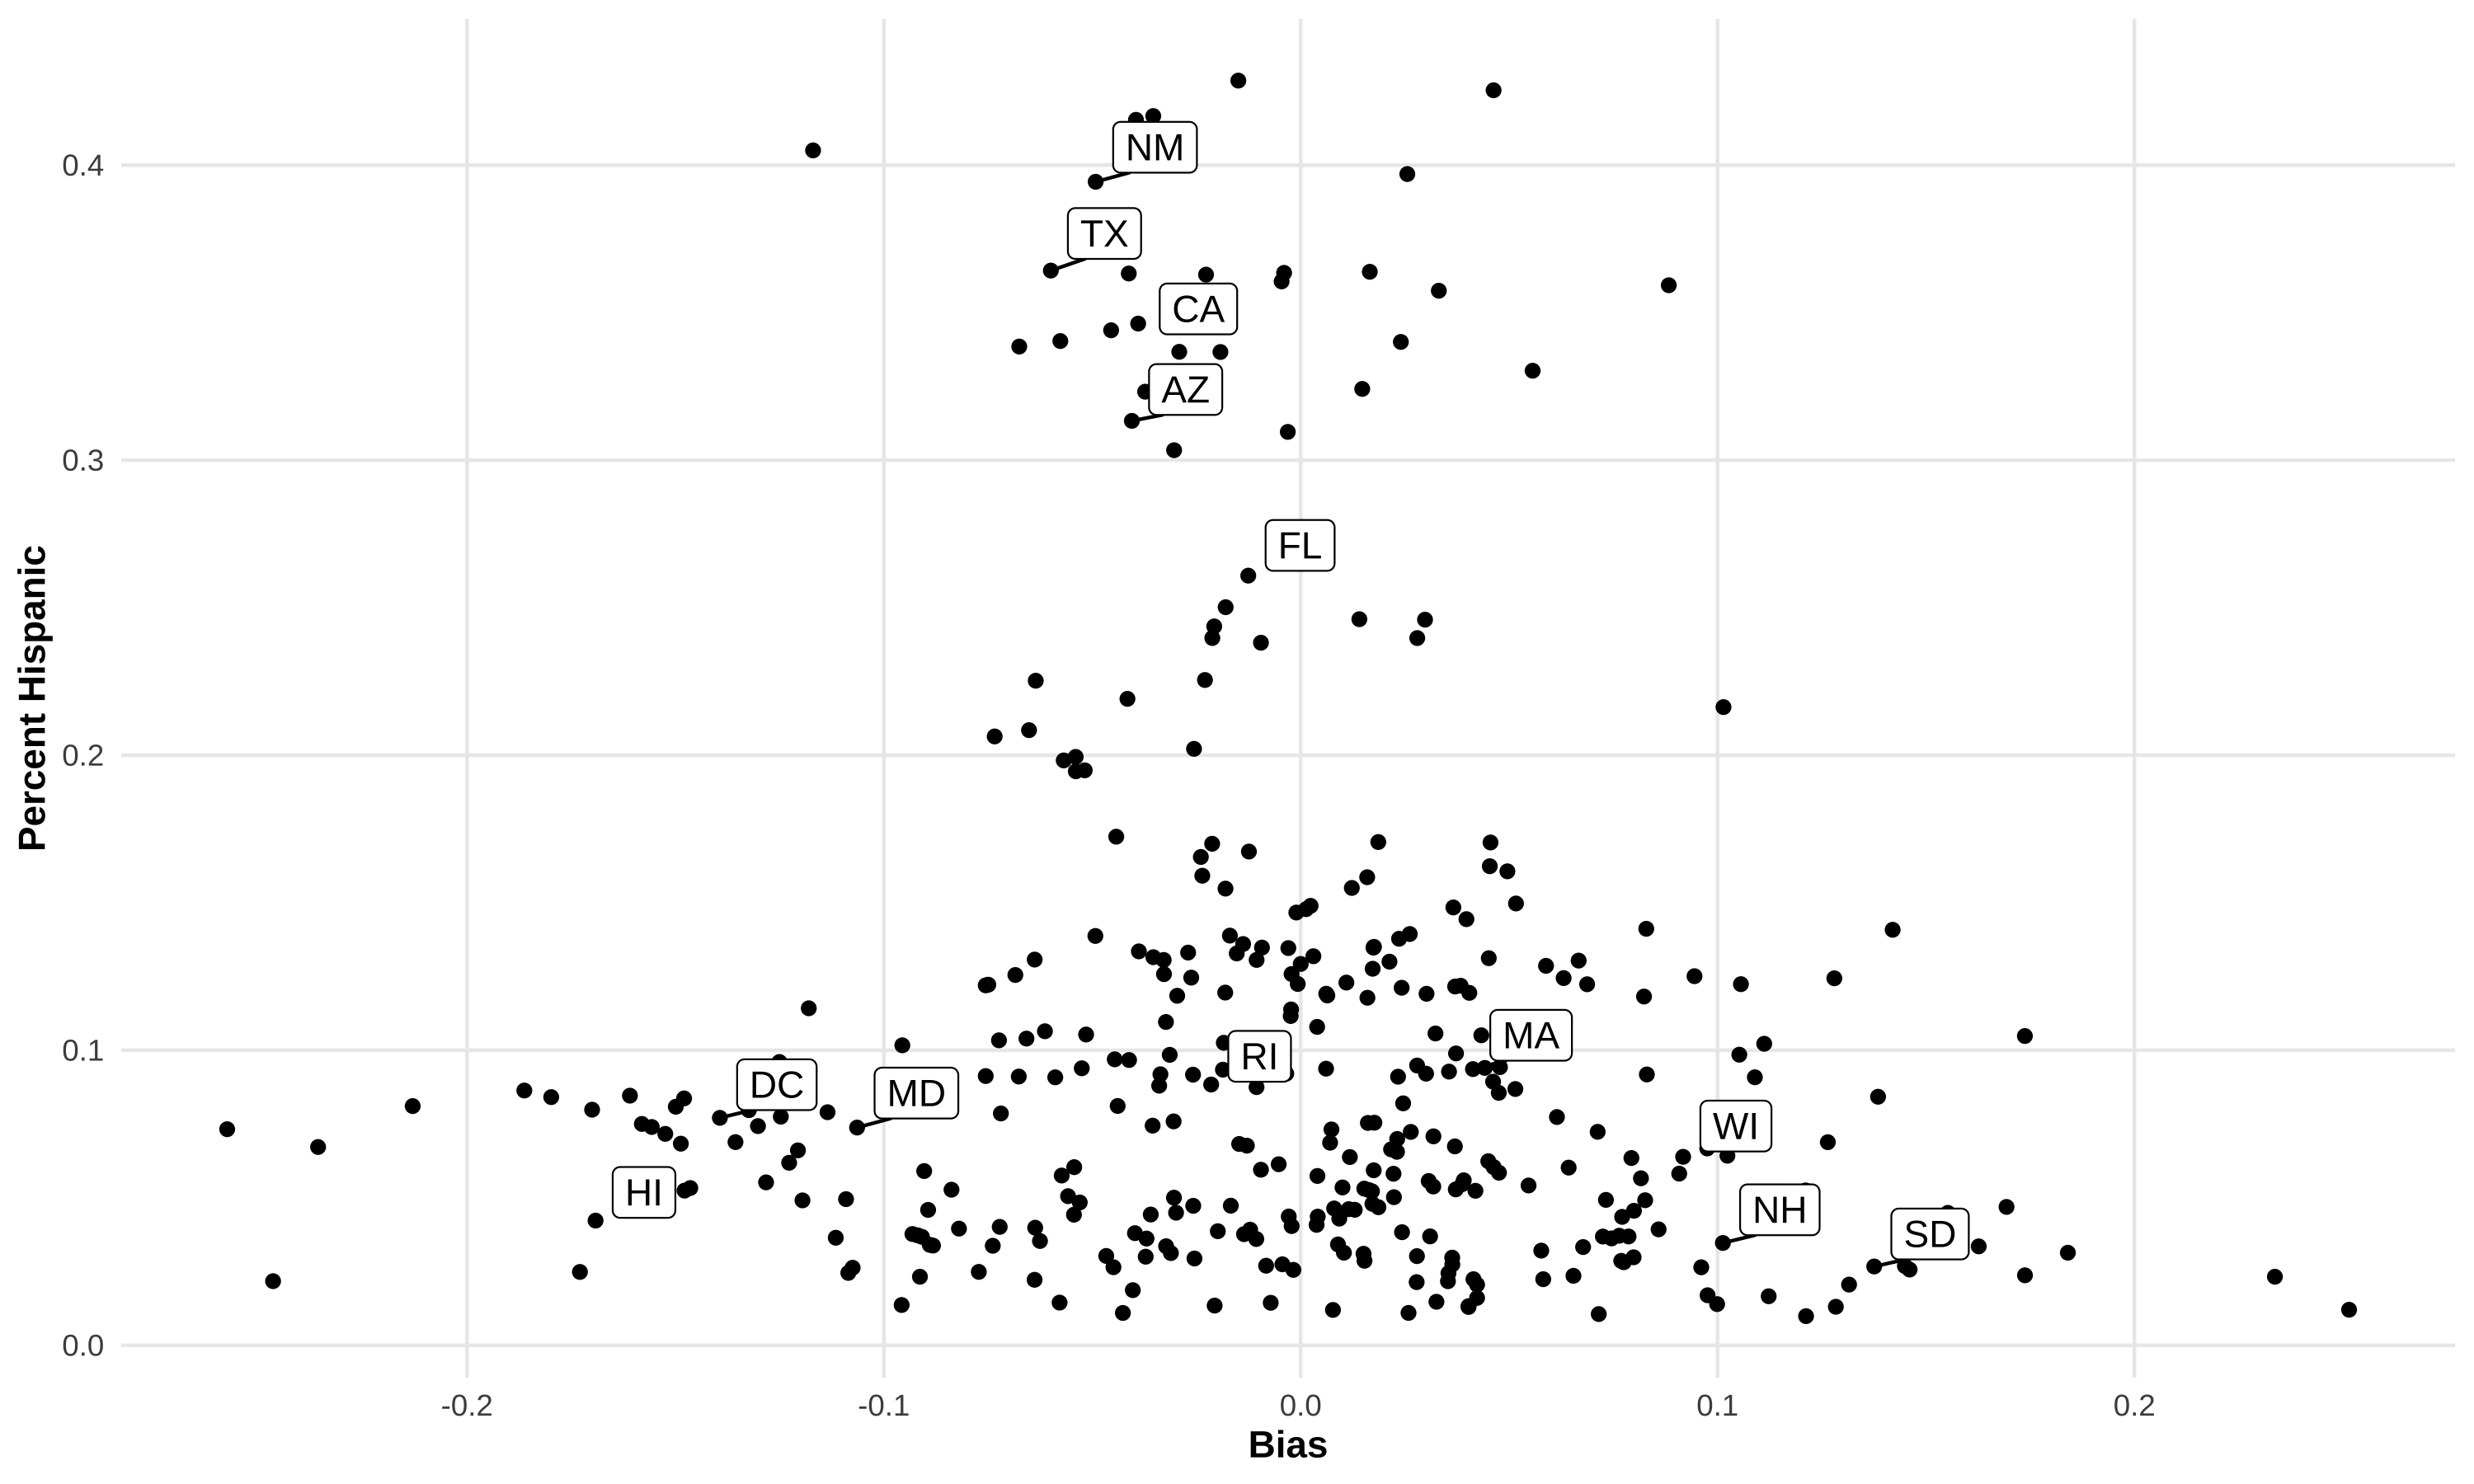
\includegraphics[width=.9\linewidth]{figure/scatter-plot-bias-hispanic-great2015.png}
\end{subfigure}
\flushleft\footnotesize{\note{Here are two scatter plots of bias on subjective Hispanic population in a state. Each dot represents a state in a certain year. Percent subjectively Hispanic = $\frac{\# \text{Hispanics}}{\text{Population}}$ \\
\emph{Source.} 2004-2021 Current Population Survey and 2004-2021 Implicit Association Test as a proxy for bias.}}
\end{figure}

\newpage
\pagebreak

\begin{figure}[!htb]
\centering
\caption{Scatter Plot of Proportion Second-Generation and Both Parents Born in a Spanish-Speaking Country on Bias}
\label{scatter-plot-4}
\begin{subfigure}{.9\textwidth}
\caption{Year < 2015}
\centering
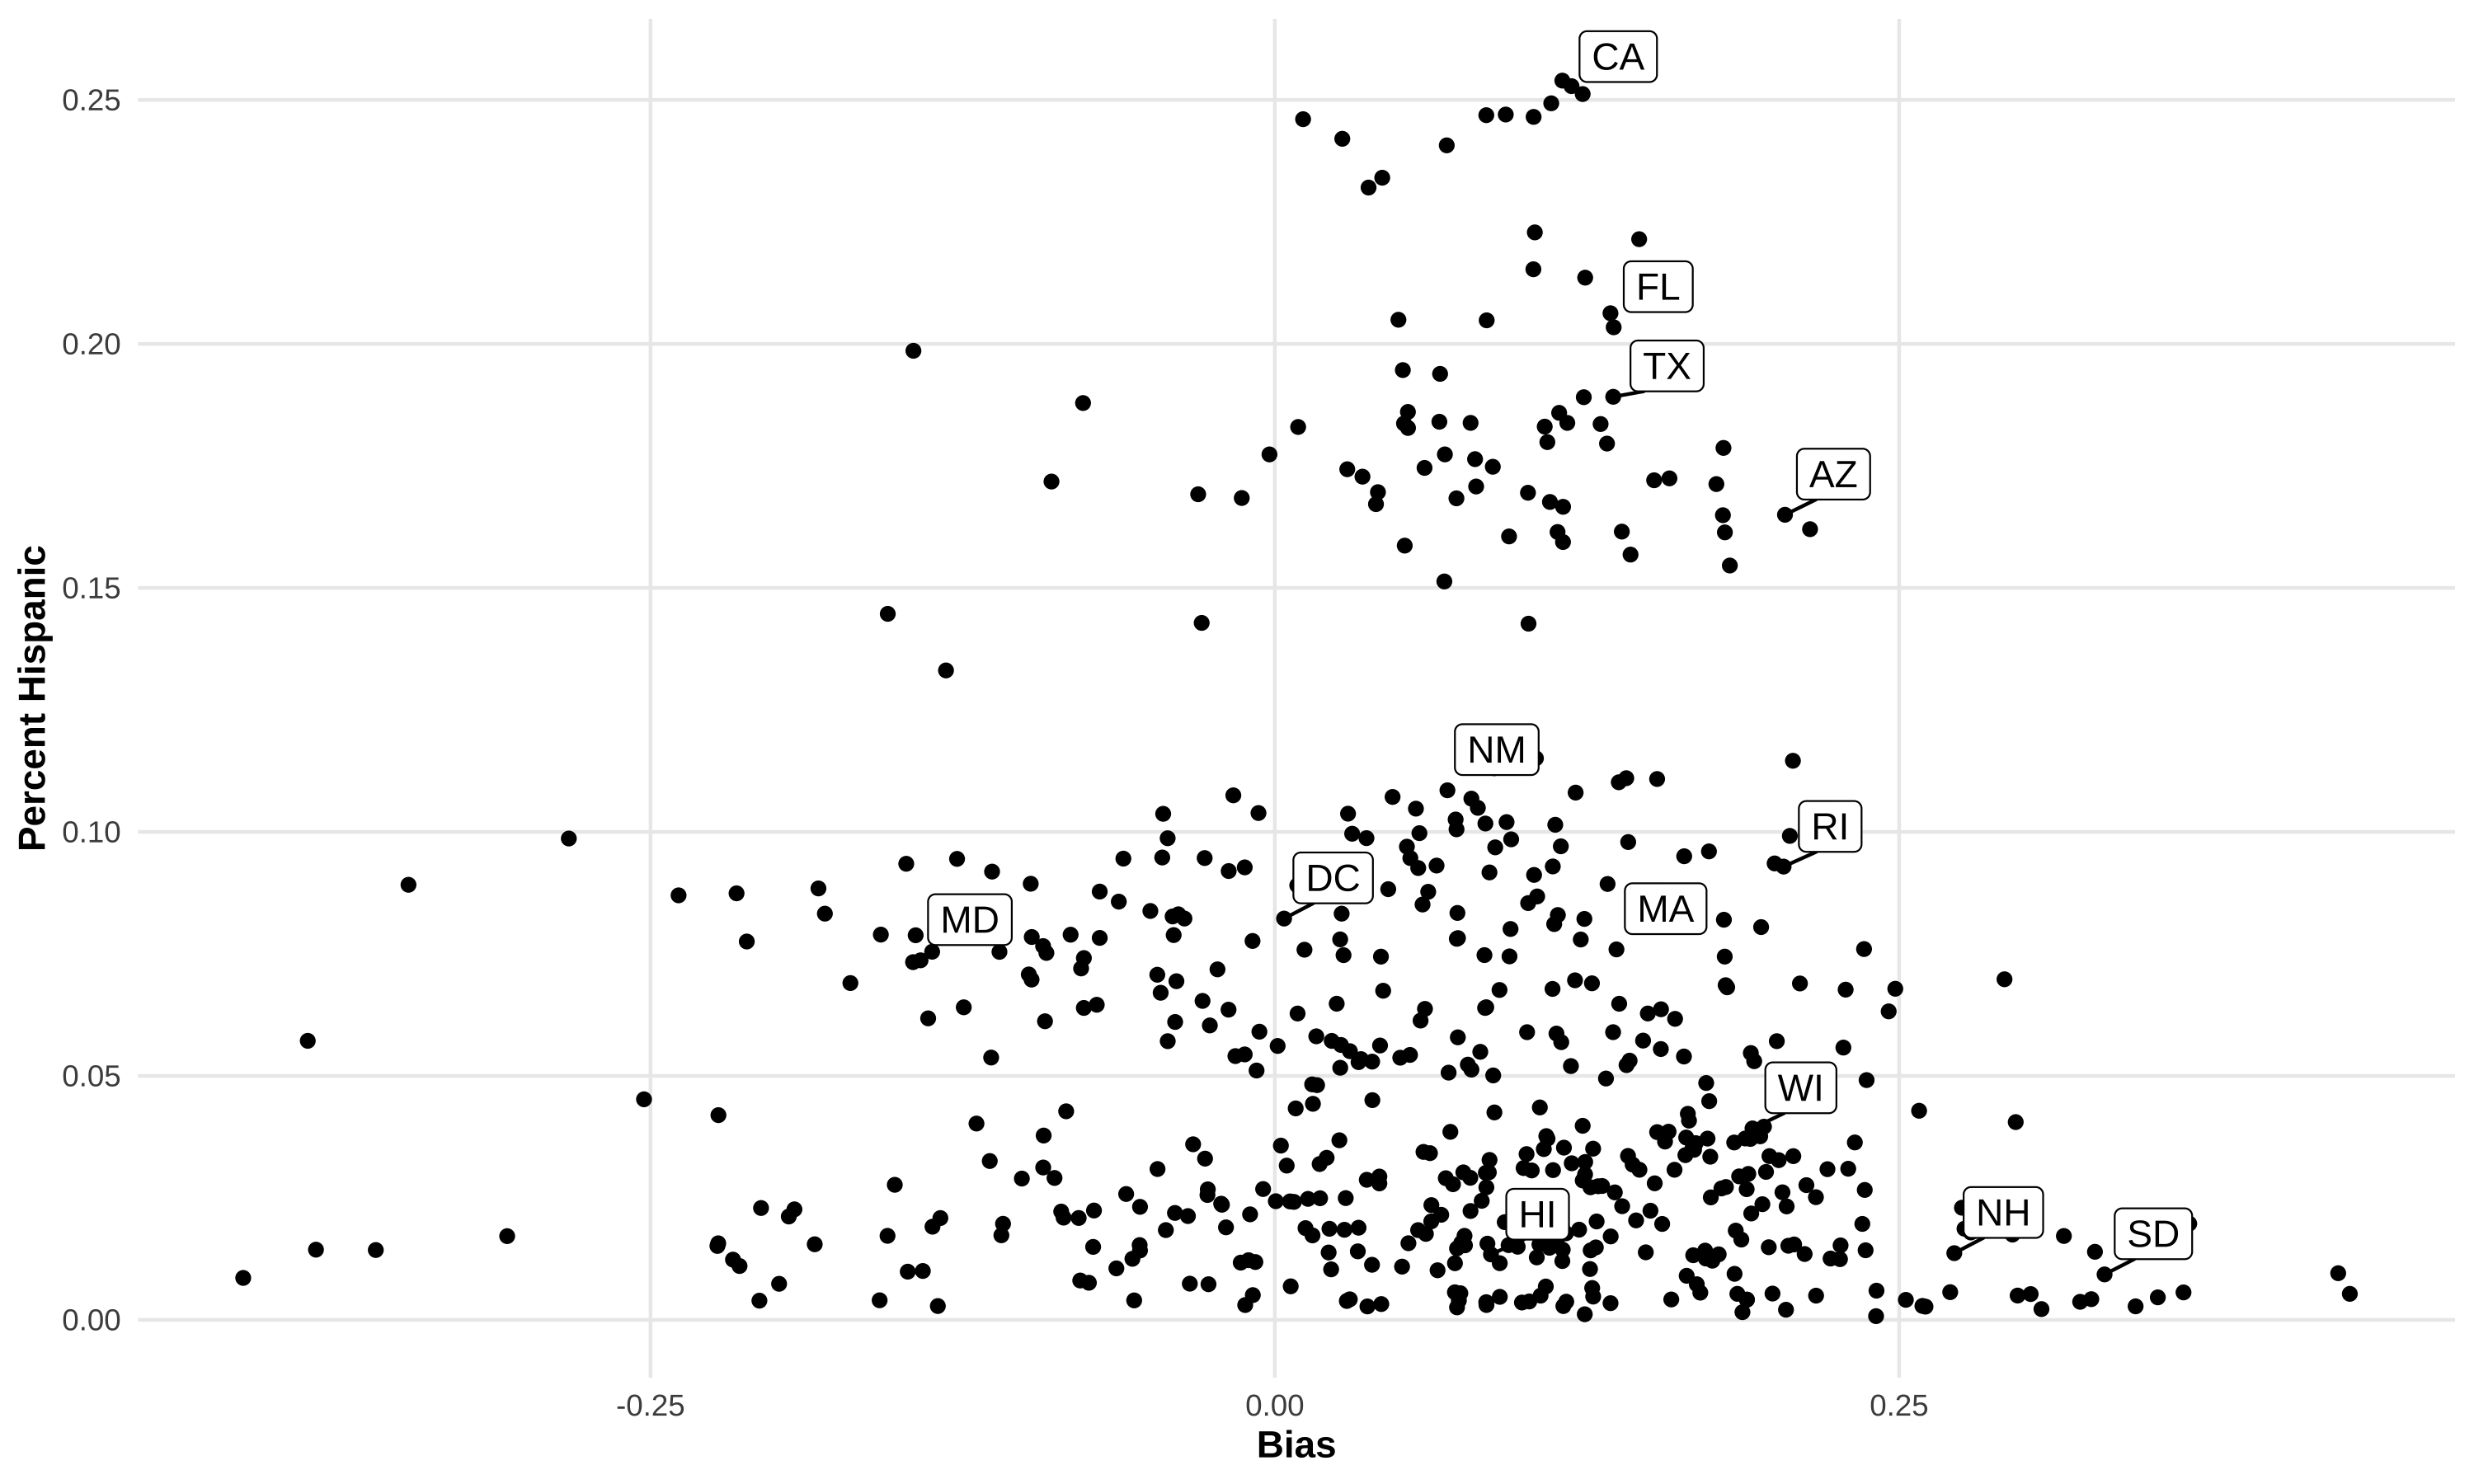
\includegraphics[width=.9\linewidth]{figure/scatter-plot-bias-hh-hispanic-less2015-hh.png}
\end{subfigure}
\centering
%Second graph
\begin{subfigure}{.9\textwidth}
\caption{Year $\geq$ 2015}
\centering
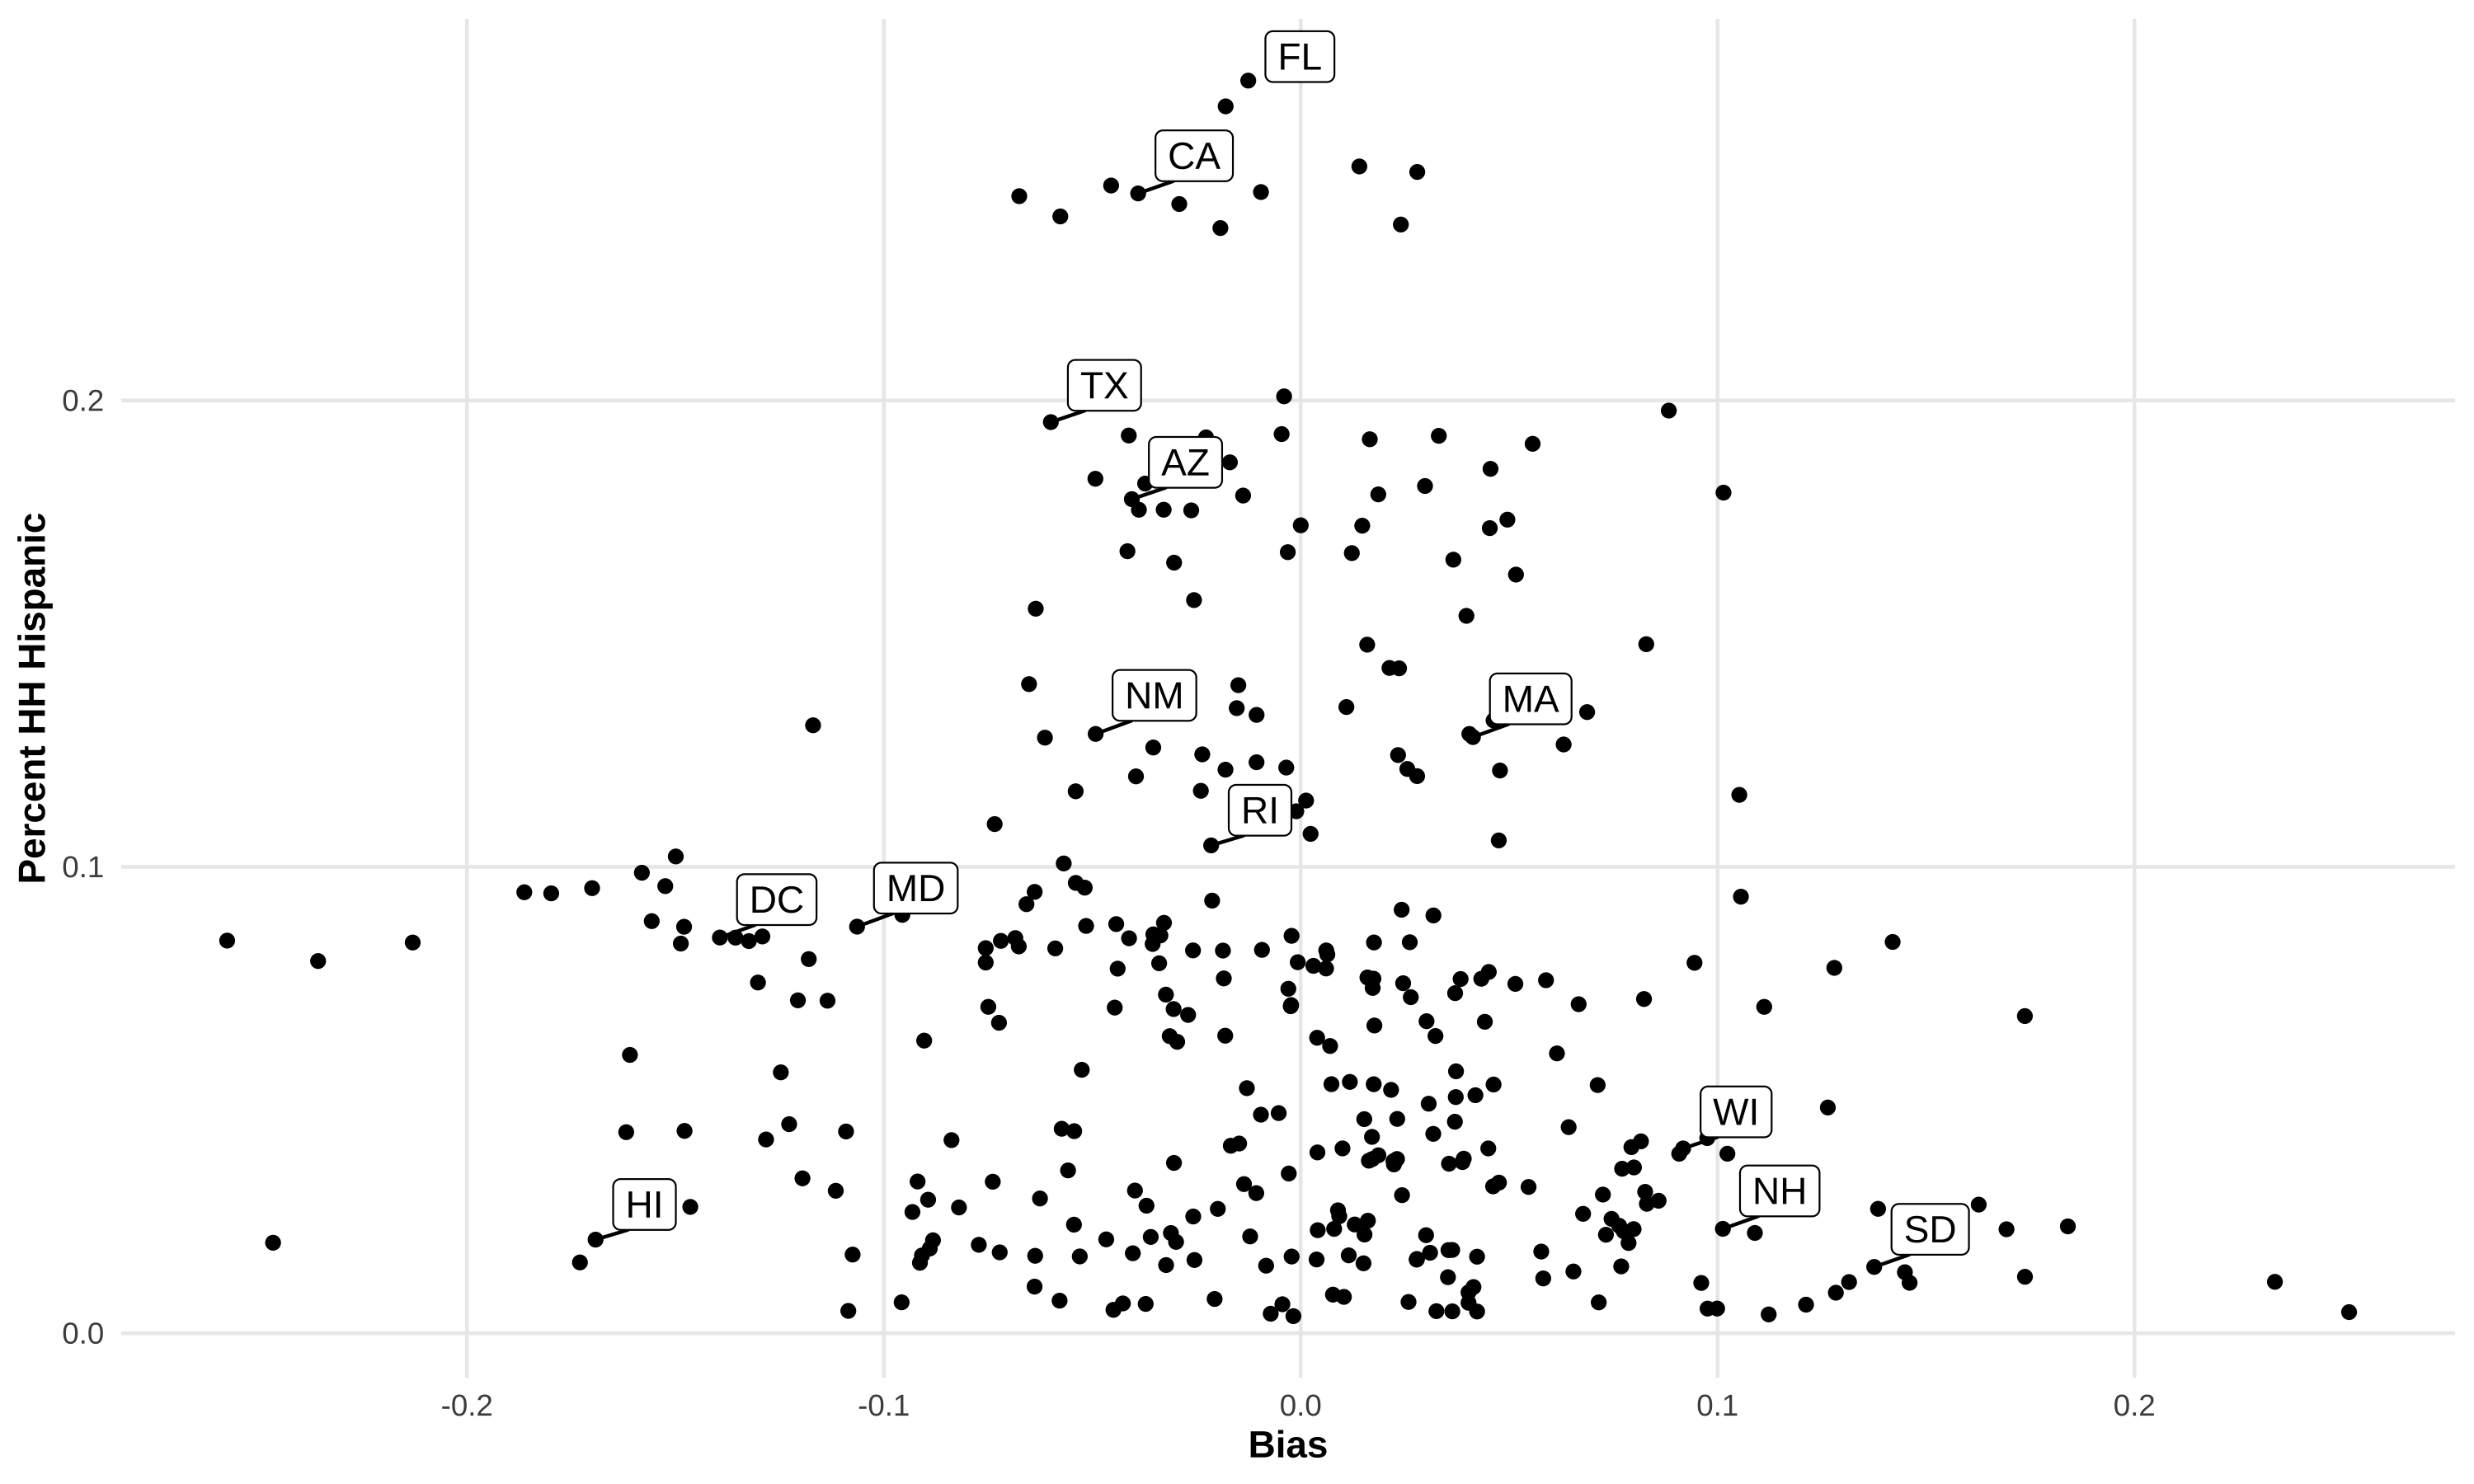
\includegraphics[width=.9\linewidth]{figure/scatter-plot-bias-hh-hispanic-great2015-hh.png}
\end{subfigure}
\flushleft\footnotesize{\note{Here are two scatter plots of bias on subjective Hispanic population in a state. Each dot represents a state in a certain year. \\ Percent HH Hispanic = $\frac{\# \text{Hispanics with two parents born in a Spanish-speaking country}}{\text{Population}}$. \\
\emph{Source.} 2004-2021 Current Population Survey and 2004-2021 Implicit Association Test as a proxy for bias.}}
\end{figure}

% \newpage
% \pagebreak


% \begin{figure}[!htb]
% \centering
% \caption{Scatter Plot of Non-Hispanic Second-Generation Hispanic-Hispanic Parents on Bias}
% \label{scatter-plot-2}
% \begin{subfigure}{.9\textwidth}
% \caption{Year < 2015}
% \centering
% 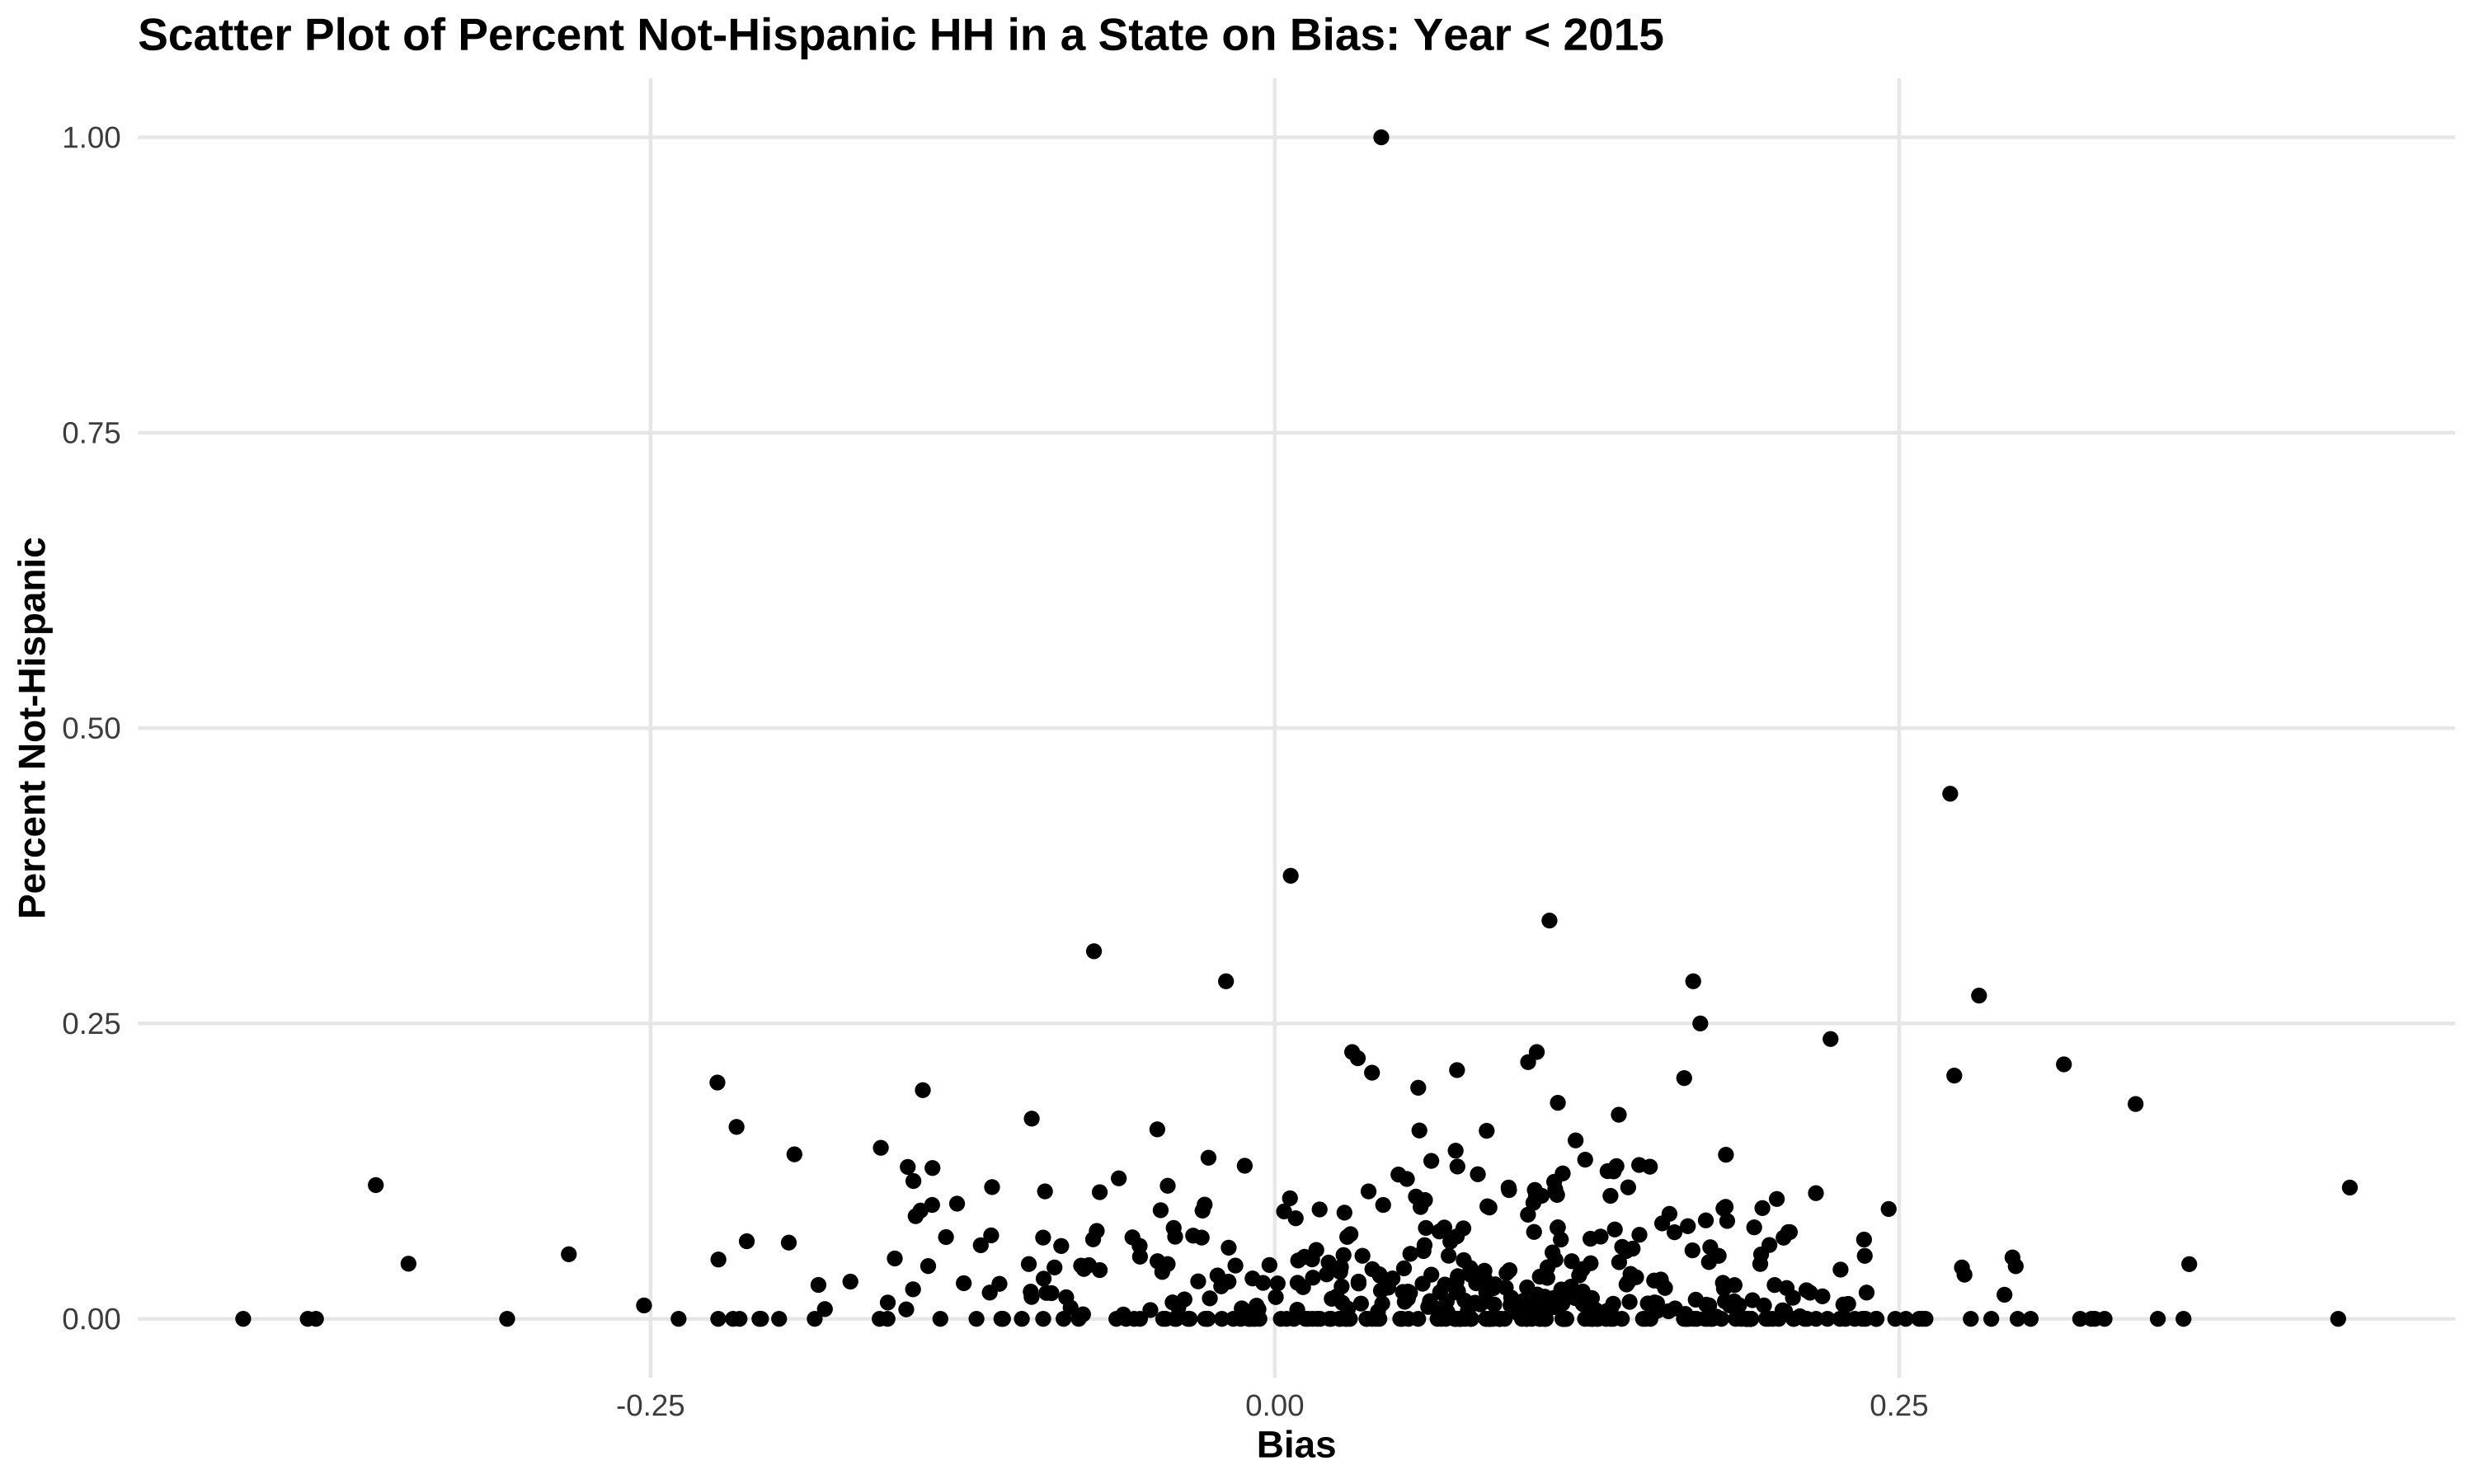
\includegraphics[width=.9\linewidth]{figure/scatter-plot-bias-hh-nothispanic-less2015.png}
% \end{subfigure}
% \centering
% %Second graph
% \begin{subfigure}{.9\textwidth}
% \caption{Year $\geq$ 2015}
% \centering
% 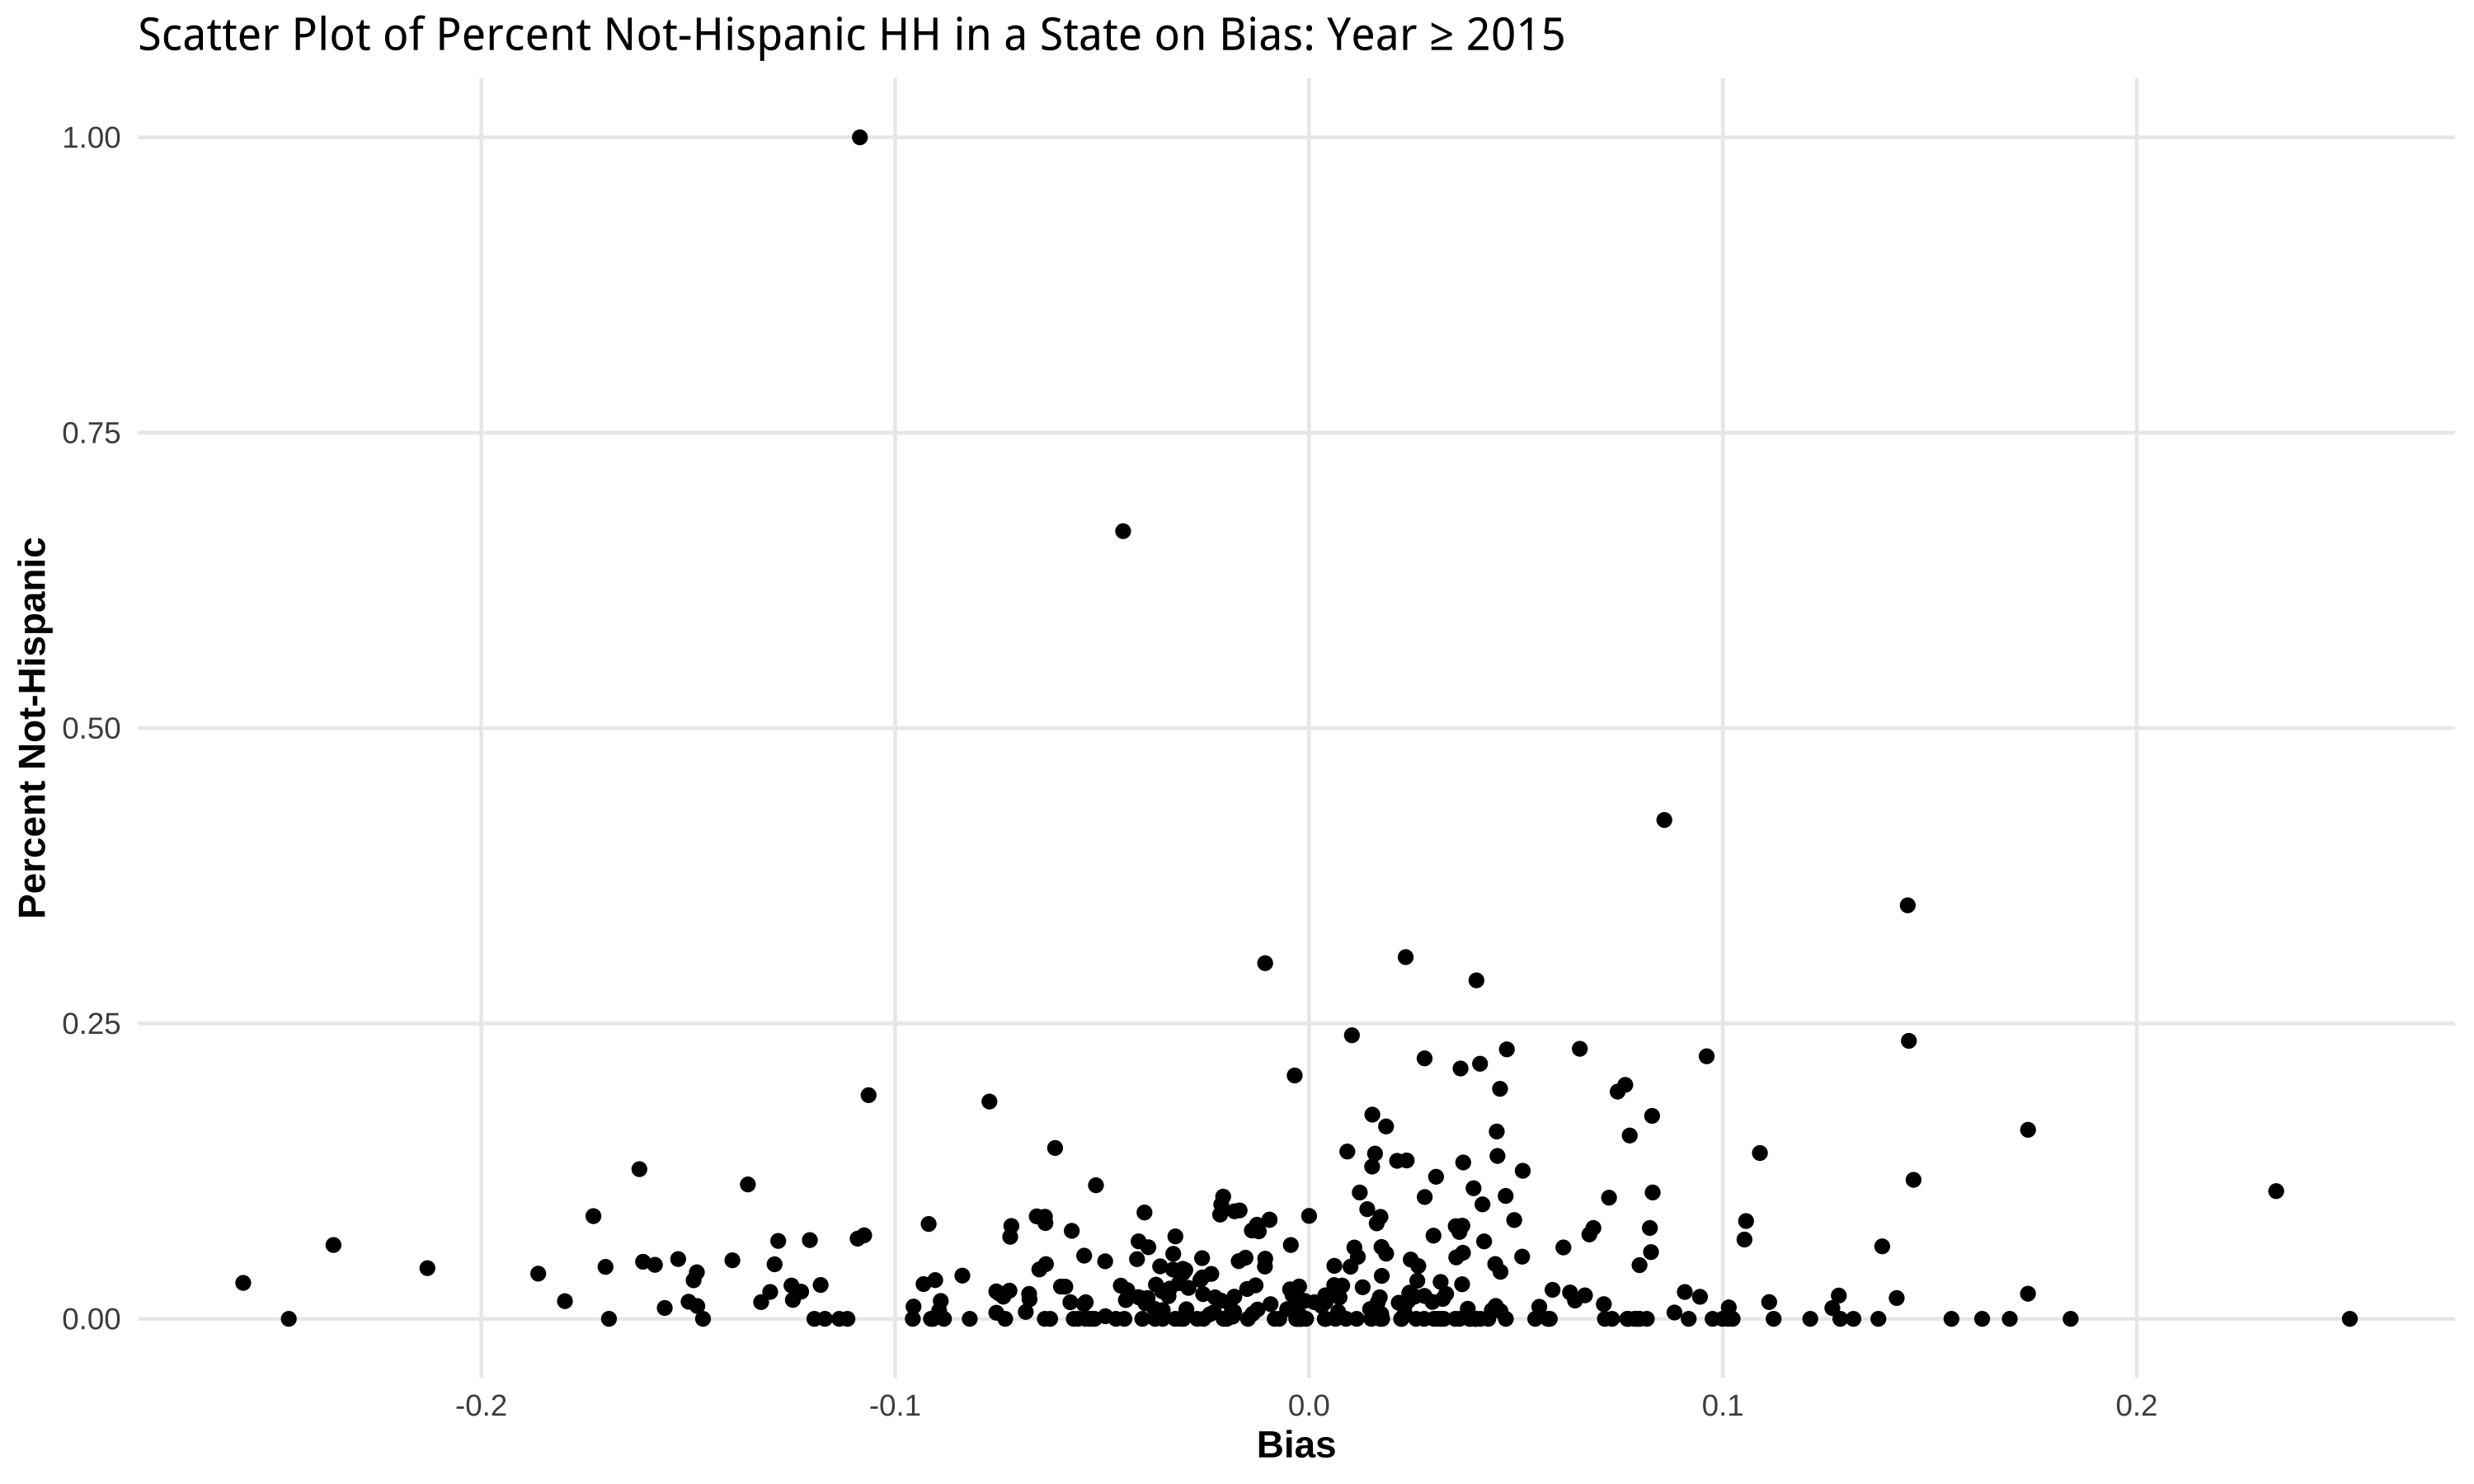
\includegraphics[width=.9\linewidth]{figure/scatter-plot-bias-hh-nothispanic-great2015.png}
% \end{subfigure}
% \end{figure}

% \newpage
% \pagebreak


\section{Data} % (fold)
\label{sec:data-ap}


\begin{figure}[!htb]
\centering
\caption{Examples of an Implicit Association Test}
\label{fig:iatexamples}
\begin{subfigure}{.48\textwidth}
\centering
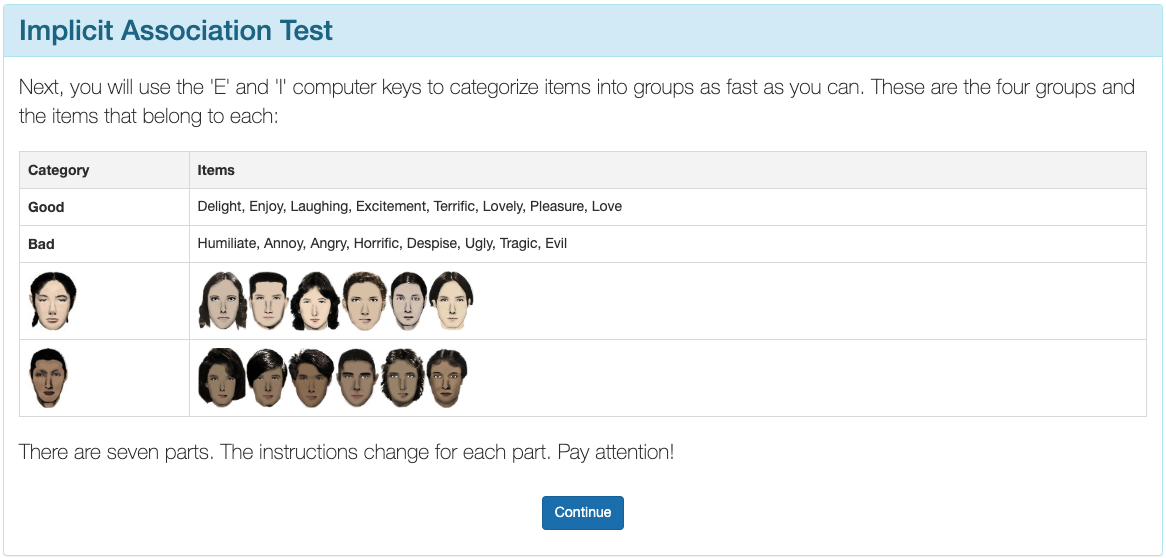
\includegraphics[width=.9\linewidth]{figure/iatexample1.png}
\end{subfigure}
\centering
%Second graph
\begin{subfigure}{.48\textwidth}
\centering
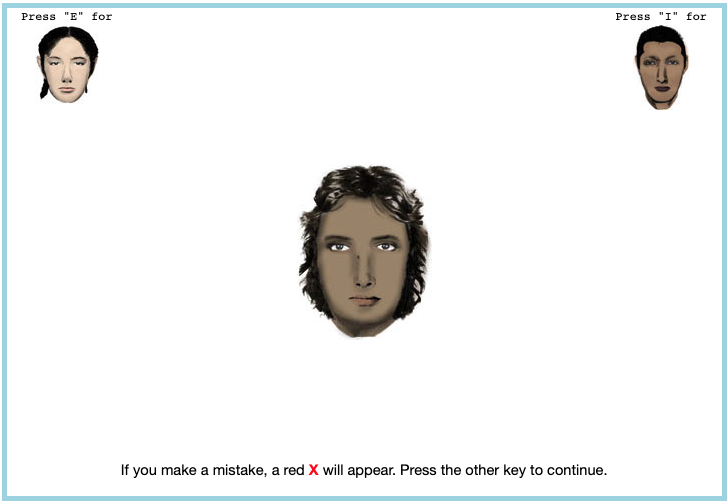
\includegraphics[width=.9\linewidth]{figure/iatexample2.png}
\end{subfigure}
%Third
\begin{subfigure}{.48\textwidth}
\centering
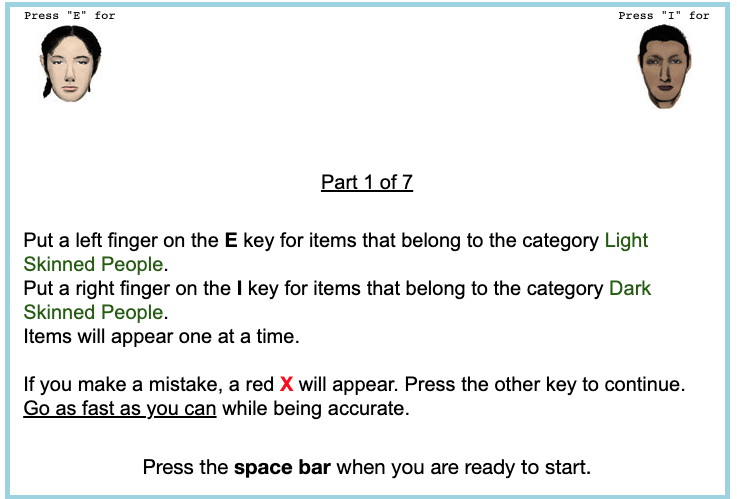
\includegraphics[width=.9\linewidth]{figure/iatexample3.png}
\end{subfigure}
% Fourth
\begin{subfigure}{.48\textwidth}
\centering
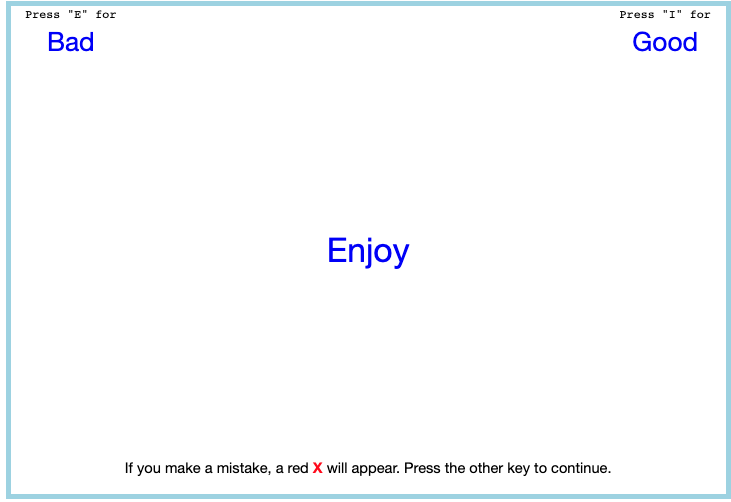
\includegraphics[width=.9\linewidth]{figure/iatexample4.png}
\end{subfigure}
%Fifth
\begin{subfigure}{.48\textwidth}
\centering
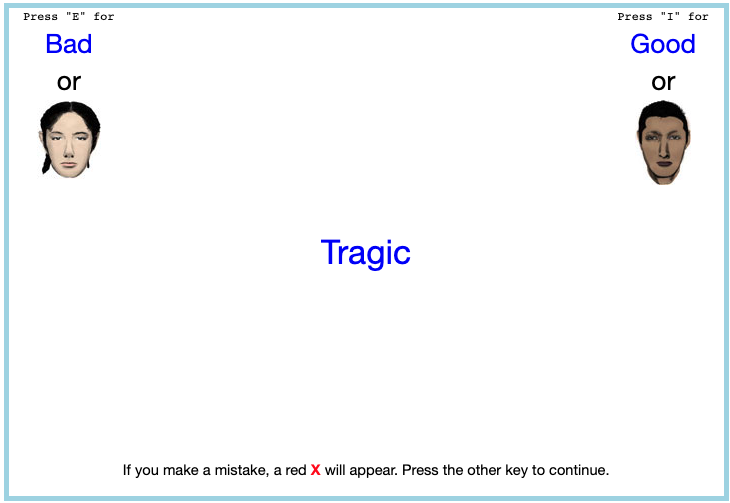
\includegraphics[width=.9\linewidth]{figure/iatexample5.png}
\end{subfigure}
\flushleft\footnotesize{\note{Here are a few examples of what a respondent would see on an implicit association test.}}
\end{figure}

\end{appendices}

\newpage
\pagebreak


\bibliography{AttitudesPaper}

\end{document}